\documentclass[9pt,dvipsnames]{beamer}

\usepackage{packages_beamer}
\addbibresource{bibliography.bib}

% Presentation Metadata
\author[Luis Palacios]{Luis Palacios}
\title[G-CNNs and Low Coherence MLPs]{\texorpdfstring{%
	{
		\bf \fontsize{25}{25}
		\selectfont 
		GROUP EQUIVARIANT CNNs AND \\ LOW COHERENCE MLPs \\
		\vspace{0.1em}
		{
			\fontsize{10}{10}\selectfont \href{https://github.com/luispky/AdvancedDeepLearning-UniTS/tree/main/final_project}{\faGithub}
		} \\
		\vspace{0.3em}
			{
				\fontsize{12}{12}\selectfont Advanced Deep Learning \\
			}
		\vspace{-0.5em}
	}
}{
	GROUP EQUIVARIANT CNNs AND LOW COHERENCE MLPs - Advanced Deep Learning
}}

\institute[UniTS]{%
    {\normalsize University of Trieste \vspace{-0.5em}}
}
\date[July 2025]{July 2025}


%--------------------------------------------------------------------------------------
\begin{document}

% Title Page
\begin{frame}
	\titlepage
\end{frame}

%--------------------------------------------------------------------------------------
\section{Introduction}
\begin{frame}{Introduction}

	\textbf{Convolutional Neural Networks are equivariant to translations but not to other transformations.}

	\begin{figure}[H]
		\centering
		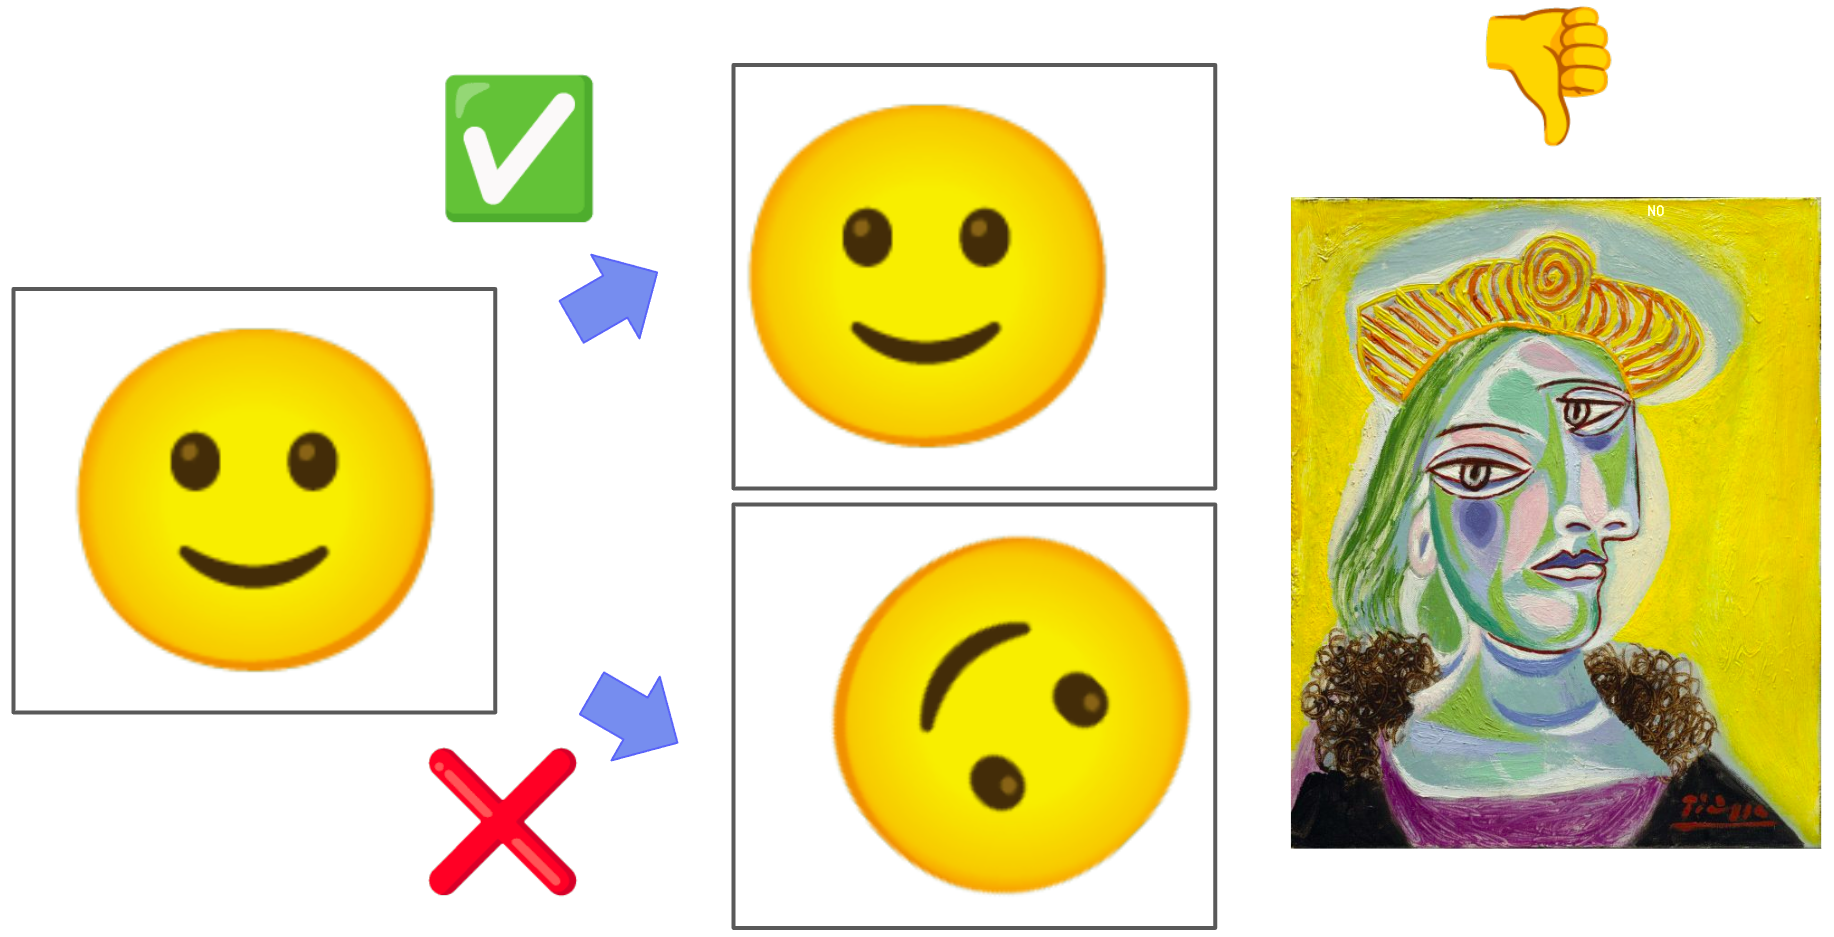
\includegraphics[width=\textwidth]{images/g-cnn_motivation.png}
		\label{fig:intro}
	\end{figure}

\end{frame}
%--------------------------------------------------------------------------------------
\section{Outline}
\begin{frame}{Outline}

	\tableofcontents

\end{frame}
%--------------------------------------------------------------------------------------
\section{Part I: Group Equivariant Convolutional Neural Networks}
\begin{frame}[c]

	\centering
	\Huge \textbf{Part I: Group Equivariant Convolutional Neural Networks}

\end{frame}
%--------------------------------------------------------------------------------------
\subsection{Regular Convolutional Neural Networks}
\begin{frame}{Convolutional Neural Networks (CNNs)}

	\textbf{Notation}

	Here we model images and signals in general as functions $f: \mathbb{R}^d \to \mathbb{R}^K$, with $K$ the number of channels of an image or general signal. For simplicity we take $K=1$, unless specified. We will focus on the space of square integrable functions, $L^2(\mathbb{R}^d)$.

	\sectionvspace

	\textbf{Convolution Operation}

	\begin{equation}
		(k * f)(x) = \int_{\mathbb{R}^d} \dd x' \; k(x - x') f(x')
	\end{equation}

	\textbf{Cross-Correlation Operation}

	\begin{equation}
		(k \star f)(x) = \int_{\mathbb{R}^d} \dd x' \; k(x'-x) f(x') = (\mathcal{K} f)(x)
	\end{equation}

	where

	\begin{itemize}
		\item $k \in L^1(\mathbb{R}^d)$ is a kernel function and,
		\item $\mathcal{K}: L^2(\mathbb{R}^d) \to L^2(\mathbb{R}^d)$ is a linear and bounded operator, which will be useful later.
	\end{itemize}

	{\color{red}\textbf{Note:} Here we refer to the convolution operation as the cross-correlation operation, which is more common in the literature. Furthermore, these two operations are intertwined in the forward and backward passes of a CNN.}

\end{frame}

%--------------------------------------------------------------------------------------
\subsection{Group Equivariant Convolutional Neural Networks}
\begin{frame}{Convolution Operation as Template Matching}

	The convolution (correlation) operator can be seen as defined by the left representation of the translation group $\mathscr{L}_x \in \mathrm{Hom}(\mathbb{R}^d, \mathcal{U}(L^2(\mathbb{R}^d)))$. Furthermore, the convolution operation can be interpreted as a form of template matching, where we slide a kernel $k$ over the input function $f$ to produce a new function.
	\begin{equation}
		\begin{split}
			(k * f)(x) & = \int_{\mathbb{R}^d} \dd x' \; k(x'-x) f(x')       \\
			           & = \int_{\mathbb{R}^d} \dd x' \; k(x^{-1}x') f(x')   \\
			           & = \braket{\mathscr{L}_x \;k}{f}_{L^2(\mathbb{R}^d)} \\
			           & = (\mathcal{K} f)(x)
		\end{split}
	\end{equation}

	where we leverage the fact that $\mathbb{R}^d$ is a G-space of the $(\mathbb{R}^d, +)$ group, and that $k$ and $f$ are functions defined on $\mathbb{R}^d$ and thus it makes sense that the left regular representation $\mathscr{L}_x$ acts on $k$.

	\sectionvspace

	{\color{red} {\bf Note:} Here we use $*$ because the (cross-)correlation operation is nothing more that the convolution operation with a reflected kernel, i.e., $k(x) = k(-x) =  k^{*}(x)$. This operation is called involution.}

	\begin{equation*}
		k * f = k^{*} \star f
	\end{equation*}

\end{frame}
%--------------------------------------------------------------------------------------
\begin{frame}{Equivariance of the convolution operation}
	\begin{alertblock}{\textbf{The convolution operation is an equivariant map for the translation group}}
		\begin{equation*}
			\begin{split}
				(k *_{\mathbb{R}^d} \mathscr{L}_t f)(x) & = \int_{\mathbb{R}^d} \dd x' \; k(x^{-1}x') \mathscr{L}_t f(x')                                                                            \\
				                                        & = \braket{\mathscr{L}_x \;k}{\mathscr{L}_t f}_{L^2(\mathbb{R}^d)}                                                                          \\
				                                        & = \braket{\mathscr{L}_{t^{-1}} \mathscr{L}_x \;k}{ f}_{L^2(\mathbb{R}^d)} = \braket{\mathscr{L}_{t^{-1} \; x} \;k}{ f}_{L^2(\mathbb{R}^d)} \\
				                                        & = \int_{\mathbb{R}^d} \dd x' \; k(x^{-1}t\;x') f(x')                                                                                       \\
				                                        & = (k *_{\mathbb{R}^d} f)(t^{-1}x)                                                                                                          \\
				                                        & = [\mathscr{L}_t (k *_{\mathbb{R}^d} f)](x)                                                                                                \\
			\end{split}
		\end{equation*}

		{\color{orange} {\bf Remark:} $\dd x' = \dd(t x')$ because $\dd x'$ is the left Haar measure, which is an invariant measure on the group.}
	\end{alertblock}

	\textbf{Note:} The convolution operation is not an equivariant map for the group of rotations because a representation $\mathscr{L}_t \in \mathrm{Hom}(SO(d), \mathcal{U}(L^2(SO(d)))$ whereas the kernel function $k$  and the input function $f$ are defined on $\mathbb{R}^d$. Thus, the convolution operation does not preserve the equivariance property for rotations.

\end{frame}
%--------------------------------------------------------------------------------------
\begin{frame}{Group Equivariant Neural Networks}

	\begin{block}{\bf Group Equivariant Convolutional Neural Networks (G-CNNs)}
		\begin{equation}
			\begin{split}
				(k *_{G} f)(g) & = \int_G \dd g' \; k(g^{-1} g') f(g')                          \\
				               & = \braket{\mathscr{L}_g \; k}{f}_{L^2(G)} = (\mathcal{K} f)(g)
			\end{split}
		\end{equation}
		with $\mathcal{K} = L^2(G) \to L^2(G)$ the group correlation operator.
	\end{block}

	\begin{block}{\bf Lifting-Correlation {\color{red} (The link)}}
		\begin{equation}
			\begin{split}
				(k *_{G} f)(g) & = \int_{\mathbb{R}^d} \dd x' \; k(g^{-1} x') f(x')                                      \\
				               & = \int_{\mathbb{R}^d} \dd x' \; k(h^{-1}x^{-1} x') f(x')                                \\
				               & = \int_{\mathbb{R}^d} \dd x' \; \mathscr{L}_h \; k(x^{-1} x') f(x')                     \\
				               & = \braket{\mathscr{L}_x \mathscr{L}_h \; k}{f}_{L^2(\mathbb{R}^d)} = (\mathcal{K} f)(g)
			\end{split}
		\end{equation}
		with $g = (x, h)$ and $\mathcal{K} = L^2(\mathbb{R}^d) \to L^2(G)$ the lifting correlation operator.
	\end{block}

\end{frame}
%--------------------------------------------------------------------------------------
\begin{frame}{Summary of Equivariant Layers}

	\begin{alertblock}{Theorem}
		A linear layer between feature maps is equivariant if and only if it is a group convolutions.

		Reference: \cite{bekkers_uvagedl}
	\end{alertblock}

	\begin{block}{Summary}
		In a nutshell, we can differentiate the types of equivariant layers by:
		\begin{itemize}
			\item convolution operator $\mathcal{K}: L^2(X) \to L^2(Y)$
			\item the linear part $H$ of the group $G$, which adds restrictions to the kernel function $k$
		\end{itemize}
	\end{block}

	\begin{block}{Limitations of G-CNNs}
		\begin{itemize}
			\item The group $G$ must be finite and the convolutions need to be discrete.
		\end{itemize}
	\end{block}

\end{frame}

%--------------------------------------------------------------------------------------
\begin{frame}{Workflow for working with GCNNs}

	\begin{figure}[H]
		\centering
		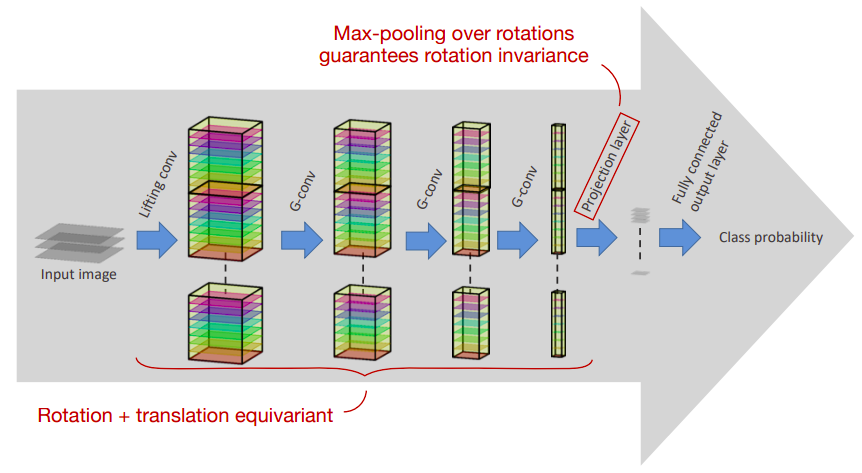
\includegraphics[width=\textwidth]{images/g-cnn_workflow.png}
		\label{fig:g-ccn_workflow}
	\end{figure}
	Reference: \cite{bekkers_uvagedl}

\end{frame}
%--------------------------------------------------------------------------------------
\begin{frame}{Practical Convolution Filter Implementation}

	\textbf{Planar Convolution}

	For the translation group in $G = (\mathbb{Z}^2, +)$, we have:

	\begin{itemize}
		\item input feature maps shape at layer $l$: $K^\ell \times H \times W$
		\item output feature maps shape at layer $l+1$ : $K^{\ell+1} \times H' \times W'$
		\item layer filter weights shape at layer $l$ : $K^{\ell+1} \times K^\ell \times \tilde{H} \times \tilde{W}$
	\end{itemize}

	\textbf{Group Convolution}

	For an affine group $G = \mathbb{R}^d \rtimes H$, we have:

	\begin{itemize}
		\item input feature maps shape at layer $l$: $K^\ell \times S^{\ell} \times H \times W$
		\item output feature maps shape at layer $l+1$ : $K^{\ell+1} \times S^{\ell + 1} \times H' \times W'$
		      % !TODO: check if this is correct
		\item layer filter weights shape at layer $l$ : $K^{\ell+1} \times S^{\ell} \times K^\ell \times S^{\ell} \times \tilde{H} \times \tilde{W}$
	\end{itemize}

	where:
	\begin{itemize}
		\item $K^\ell$ is the number of feature maps at layer $\ell$,
		\item $H \times W$ is the spatial dimensions of the input feature maps,
		\item $S^\ell$ is dimension of the group linear part $H$ of the feature maps at layer $\ell$,
		\item $S^\ell \times H \times W$ {\bf is the group space dimensions of the feature maps at layer $\ell$.} {\color{red} \bf Group convolutions just add the dimension of the group linear part $H$ to the feature maps.}
	\end{itemize}

\end{frame}
%--------------------------------------------------------------------------------------
\subsection{Implementation Results}
\begin{frame}{Implementation Results}

\begin{block}{Architectures}

	\begin{itemize}
		\item MLP: 1 hidden layer, 128 hidden units, dropout 0.2, batch norm, ReLU activation
		\item CNN: 4 hidden layers, 32 filters, 5x5 kernel, 1x1 stride, 0x0 padding
		\item GCNN: 4 hidden layers, 16 filters, 5x5 kernel, 1x1 stride, 0x0 padding, $C_4$ group
	\end{itemize}

\end{block}

\begin{table}[h]
\centering
\begin{tabular}{|c|c|c|c|}
\hline
\textbf{Model} & \textbf{MNIST} & \textbf{Fashion-MNIST} & \textbf{CIFAR-10} \\
\hline
MLP & 0.34, 0.98 & 0.19, 0.89 & 0.24, 0.52 \\
\hline
CNN & 0.46, \textcolor{blue}{\textbf{0.99}} & 0.22, \textcolor{blue}{\textbf{0.91}} & 0.29, \textcolor{blue}{\textbf{0.68}} \\
\hline
GCNN & \textcolor{red}{\textbf{0.92}}, 0.98 & \textcolor{red}{\textbf{0.46}}, 0.86 & \textcolor{red}{\textbf{0.35}}, 0.49 \\
\hline
\end{tabular}
\caption{Test Accuracy (T.A.) Results for Different Models and Datasets. Entries: (T.A. with data augmentation, T.A. without data augmentation)}
\label{tab:test_accuracy_results}
\end{table}

\textbf{Note:} The diehidral group $D_4$ gave issues in the \textbf{\texttt{InterpolativeGroupKernel}} implementation for the \textbf{\texttt{GroupConvolution}} layer. $D_4$ is a 2-dimensional group, $C_4$ is a 1-dimensional group.

\vspace{0.3cm}
Reference: \cite{knigge_gdl_2024}

\end{frame}
%--------------------------------------------------------------------------------------
\section{Part II: Low Coherence MLPs}
\begin{frame}

	\centering
	\Huge \textbf{Part II: Low Coherence MLPs}

\end{frame}
%--------------------------------------------------------------------------------------
\subsection{Frames and Coherence}
\begin{frame}{Frames and Coherence}

	\begin{block}{Definition: Frame}
		A \textbf{frame} is a set of vectors $\{x_i\}_{i=1}^n$ in a Hilbert space $H$ such that there exist constants $A, B > 0$ (called frame bounds) satisfying:
		\begin{equation*}
			A \|x\|^2 \leq \sum_{i=1}^N |\langle x_i, x \rangle|^2 \leq B \|x\|^2 \quad \forall \; x \in H
		\end{equation*}

		A frame generalizes the notion of a basis but allows redundancy.

		Let $H = \mathbb{R}^m$ and $X \in \mathbb{R}^{m \times n}$ be the matrix whose $i$-th column is $x_i$, i.e., $X = [x_1 \; x_2 \; \dots \; x_n]$. Then the frame condition can be written as:
		\begin{equation*}
			A \|x\|^2 \leq x^T X X^T x \leq B \|x\|^2.
		\end{equation*}
	\end{block}

	\begin{block}{Special Frame Types}
		\begin{itemize}
			\item \textbf{Unit-norm frame}: Each frame vector has unit norm: $\|x_i\| = 1$
			\item \textbf{Equiangular frame}: All pairwise inner products are equal in absolute value: $|\langle x_i, x_j \rangle| = c$ for $i \neq j$
			\item \textbf{Tight frame}: $A = B$ and $XX^T = \frac{n}{m}I_m$
		\end{itemize}
	\end{block}

	References: \cite{thill_low-coherence_2015, thill_group_2015}

\end{frame}
%--------------------------------------------------------------------------------------
\begin{frame}{Coherence and Equivariance}

	\begin{block}{Definition: Frame Coherence}
		The \textbf{coherence} of a frame is a measure of how closely packed the frame vectors are. For a matrix $X$ with frame vectors as columns, it is defined as:
		\begin{equation*}
			\mu(X) = \max_{i \neq j} |\langle x_i, x_j \rangle|
		\end{equation*}
		Lower coherence means better \textbf{spread} of vectors and \textbf{less redundancy}.
	\end{block}

	\begin{block}{Welch Bound}
		For an $m$-dimensional unit-norm frame with $n$ vectors, the \textbf{Welch bound} gives a theoretical lower bound on coherence:
		\begin{equation*}
			\mu(X) \geq \sqrt{\frac{n - m}{m(n - 1)}} = \mu_{\text{Welch}}
		\end{equation*}
		Equality is achieved iff the frame is \textbf{tight} and \textbf{equiangular}.
	\end{block}

	\begin{block}{Connection to Equivariance and Stability}
		\begin{itemize}
			\item \textbf{Low coherence frames} are more equivariant with respect to group actions, as the frame vectors are more uniformly distributed in the Hilbert space.
			\item \textbf{Tight frames} provide optimal stability and reconstruction properties with equal frame bounds $A = B$.
			\item \textbf{Combined properties}: Tight equiangular frames with low coherence achieve the Welch bound and provide optimal geometric configurations.
		\end{itemize}
	\end{block}

\end{frame}
%--------------------------------------------------------------------------------------
\subsection{Low Coherence Optimization}
\begin{frame}{Low Coherence Optimization Problem}

	\begin{block}{Upper Bound for Structured Frames}
		For unit-norm tight frames with $\kappa$ distinct inner product values (each appearing equally often), the coherence $\mu$ satisfies:
		\begin{equation*}
			\mu \leq \sqrt{\kappa} \mu_{\text{Welch}} = \mu_{\text{tight}}
		\end{equation*}
	\end{block}
	
	
	\begin{block}{Optimization Objective}
		We seek $n$ unit-norm vectors in $\mathbb{R}^m$ (columns of matrix $X$) whose worst-case inner product is as small as possible:
		\begin{equation*}
			L_{\text{coh}}(X) = \min_{X \in \mathbb{R}^{m \times n}} \max_{1 \leq i < j \leq n} \langle x_i, x_j \rangle \quad \text{subject to} \quad \|x_i\| = 1 \quad \forall i
		\end{equation*}

		\begin{center}
		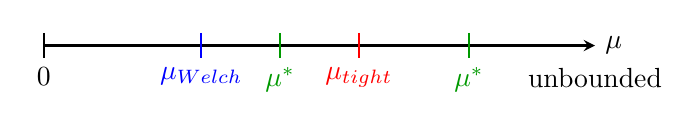
\begin{tikzpicture}[scale=2, >=stealth]
          % Draw the axis
          \draw[thick,->] (0,0) -- (3.5,0) node[right] {$\mu$};
          % Zero
          \draw[thick] (0,0.08) -- (0,-0.08);
          \node[below] at (0,-0.08) {0};
          % Welch bound
          \draw[thick,blue] (1,0.08) -- (1,-0.08);
          \node[below,blue] at (1,-0.08) {$\mu_{\text{Welch}}$};
          % Tight bound
          \draw[thick,red] (2,0.08) -- (2,-0.08);
          \node[below,red] at (2,-0.08) {$\mu_{\text{tight}}$};
          % Optimized bound between Welch and tight
          \draw[thick,green!60!black] (1.5,0.08) -- (1.5,-0.08);
          \node[below,green!60!black] at (1.5,-0.08) {$\mu^*$};
          % Optimized bound after tight
          \draw[thick,green!60!black] (2.7,0.08) -- (2.7,-0.08);
          \node[below,green!60!black] at (2.7,-0.08) {$\mu^*$};
          % Unbounded arrow
          \node[below] at (3.5,-0.08) {unbounded};
        \end{tikzpicture}
        \end{center}
	\end{block}

	\begin{block}{Rationale}
		\begin{itemize}
			\item Minimizing the maximum inner product in value (not magnitude) drives vectors to spread out maximally because lower inner products imply vectors are more widely separated.
		\end{itemize}
	\end{block}

\end{frame}
%--------------------------------------------------------------------------------------
\begin{frame}{Log-Sum-Exp Approximation}

	\begin{block}{Smooth Surrogate Function}
		Since the maximum function is non-smooth (i.e., not differentiable) and we want to minimize it using gradient descent, we use the log-sum-exp surrogate:
		\begin{equation*}
			L_{\text{coh}}(X) = \frac{1}{\lambda} \log\left( \sum_{i \neq j} \exp(\lambda \langle x_i, x_j \rangle) \right)
		\end{equation*}
		where $\lambda > 0$ is a parameter controlling approximation tightness.
	\end{block}

	Reference: \cite{wikipedia_logsumexp_2024}

	\begin{block}{Approximation Bounds}
		For $a_{ij} = \langle x_i, x_j \rangle$, the log-sum-exp satisfies:
		\begin{equation*}
			\max_{i \neq j} a_{ij} \leq L_{\text{coh}}(X) \leq \max_{i \neq j} a_{ij} + \frac{\log(n)}{\lambda}
		\end{equation*}
		As $\lambda \to \infty$, $L_{\text{coh}}(X)$ converges to the true maximum.
	\end{block}

\end{frame}
%--------------------------------------------------------------------------------------
\begin{frame}{Regularized Optimization}

	\begin{block}{Regularized Loss Function}
		We combine the coherence loss with regularization terms to encourage both equiangularity and tightness:
		\begin{equation*}
			L_{\text{total-coh}}(X) = L_{\text{coh}}(X) + \alpha \cdot L_{\text{equi}}(X) + \beta \cdot L_{\text{tight}}(X)
		\end{equation*}
		where:
		\begin{itemize}
			\item $L_{\text{equi}}(X) = \text{Var}\left(\{|\langle x_i, x_j \rangle| : i \neq j, i < j\}\right)$ encourages equiangularity
			\item $L_{\text{tight}}(X) = \|XX^T - \frac{n}{m}I_m\|_F^2$ encourages tightness
			\item $\alpha, \beta > 0$ are regularization hyperparameters
		\end{itemize}
	\end{block}

	\begin{block}{Gradient Descent Update}
		The optimization is performed via gradient descent:
		\begin{equation*}
			x_i^{(k+1)} = x_i^{(k)} - \eta \frac{\partial L_{\text{total-coh}}(X^{(k)})}{\partial x_i}
		\end{equation*}
		where $\eta$ is the learning rate and the unit-norm constraint is enforced after each step, i.e. $x_i^{(k+1)} = \frac{x_i^{(k)}}{\|x_i^{(k)}\|}$.
	\end{block}

\end{frame}
%--------------------------------------------------------------------------------------
\begin{frame}{Optimization Example: Low Coherent Frames in 2D}
	\begin{figure}[h]
		\centering
		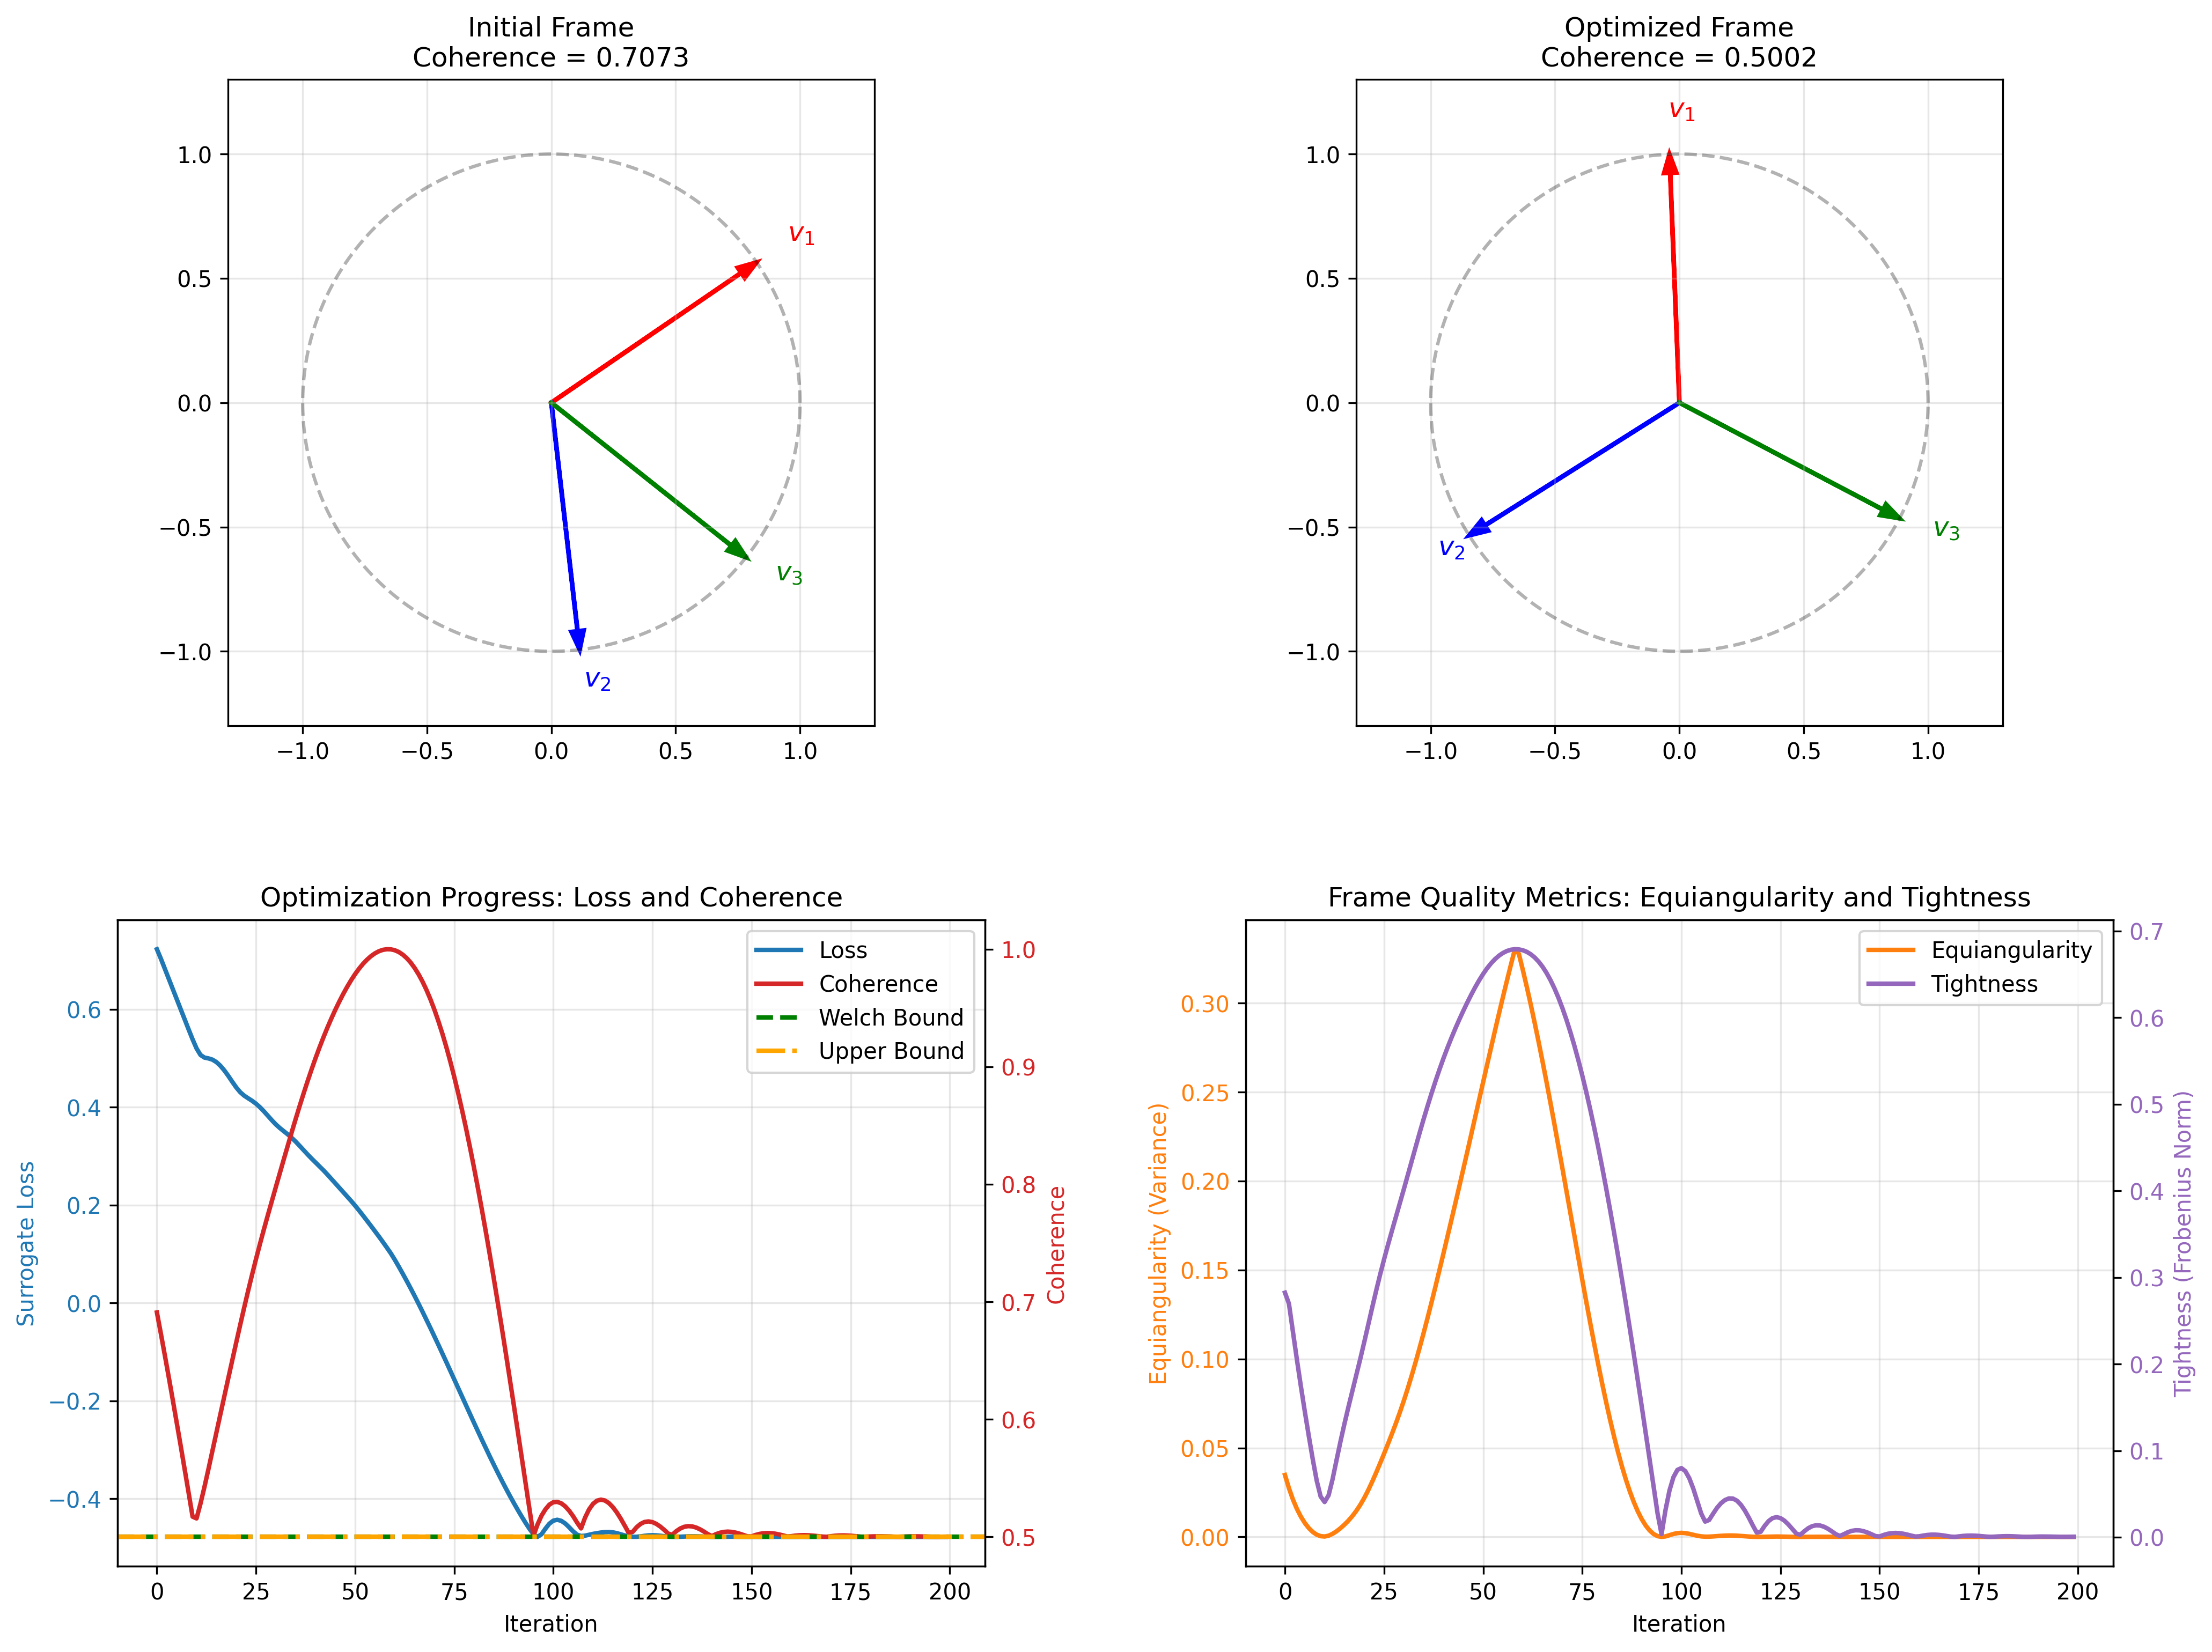
\includegraphics[width=0.95\textwidth]{../plots/frame_optimization_m2_n3_iter200_seed42_alpha0.1_beta0.1.png}
	\end{figure}
\end{frame}
%--------------------------------------------------------------------------------------
\subsection{Low Coherence MLPs}
\begin{frame}{Low Coherence MLPs Formulation}

	\begin{block}{MLP Weight Matrices as Frames}
		For each linear layer in an MLP with weight matrix $W \in \mathbb{R}^{d_{\text{out}} \times d_{\text{in}}}$:
		\begin{itemize}
			\item When $d_{\text{in}} > d_{\text{out}}$: columns of $W$ form frame vectors in $\mathbb{R}^{d_{\text{out}}}$
			\item Frame matrix: $X = W$ where $X \in \mathbb{R}^{m \times n}$ with $m = d_{\text{out}}$, $n = d_{\text{in}}$
			\item Goal: minimize coherence $\mu(W) = \max_{i \neq j} |\langle w_i, w_j \rangle|$ among weight columns
		\end{itemize}
	\end{block}

	\begin{block}{Combined Loss Function}
		The total loss combines classification and coherence objectives:
		\begin{equation*}
			L_{\text{total}}(y, \hat{y}, W) = L_{\text{original}}(y, \hat{y}) + \gamma_{\text{coh}} \sum_{l} L_{\text{total-coh}}(W^{(l)}, \lambda, \alpha, \beta)
		\end{equation*}
		where:
		\begin{itemize}
			\item $L_{\text{original}}$ is the original loss function for the task at hand, e.g. cross-entropy
			\item $L_{\text{total-coh}}$ is the coherence loss function, see previous slides, and $\lambda, \alpha, \beta$ are shared hyperparameters for all layers
			\item $\gamma_{\text{coh}} > 0$ is the coherence regularization weight
			\item Sum is over all linear layers $l$ with weight matrices $W^{(l)}$
		\end{itemize}
	\end{block}

\end{frame}
%--------------------------------------------------------------------------------------
\subsection{Implementation Results}
\begin{frame}{Implementation Results: CIFAR10}

    % 2-column figure: baseline (left), coherence model (right, stacked)
    
    \begin{figure}[H]
        \centering
        \begin{minipage}[b]{0.48\textwidth}
            \centering
            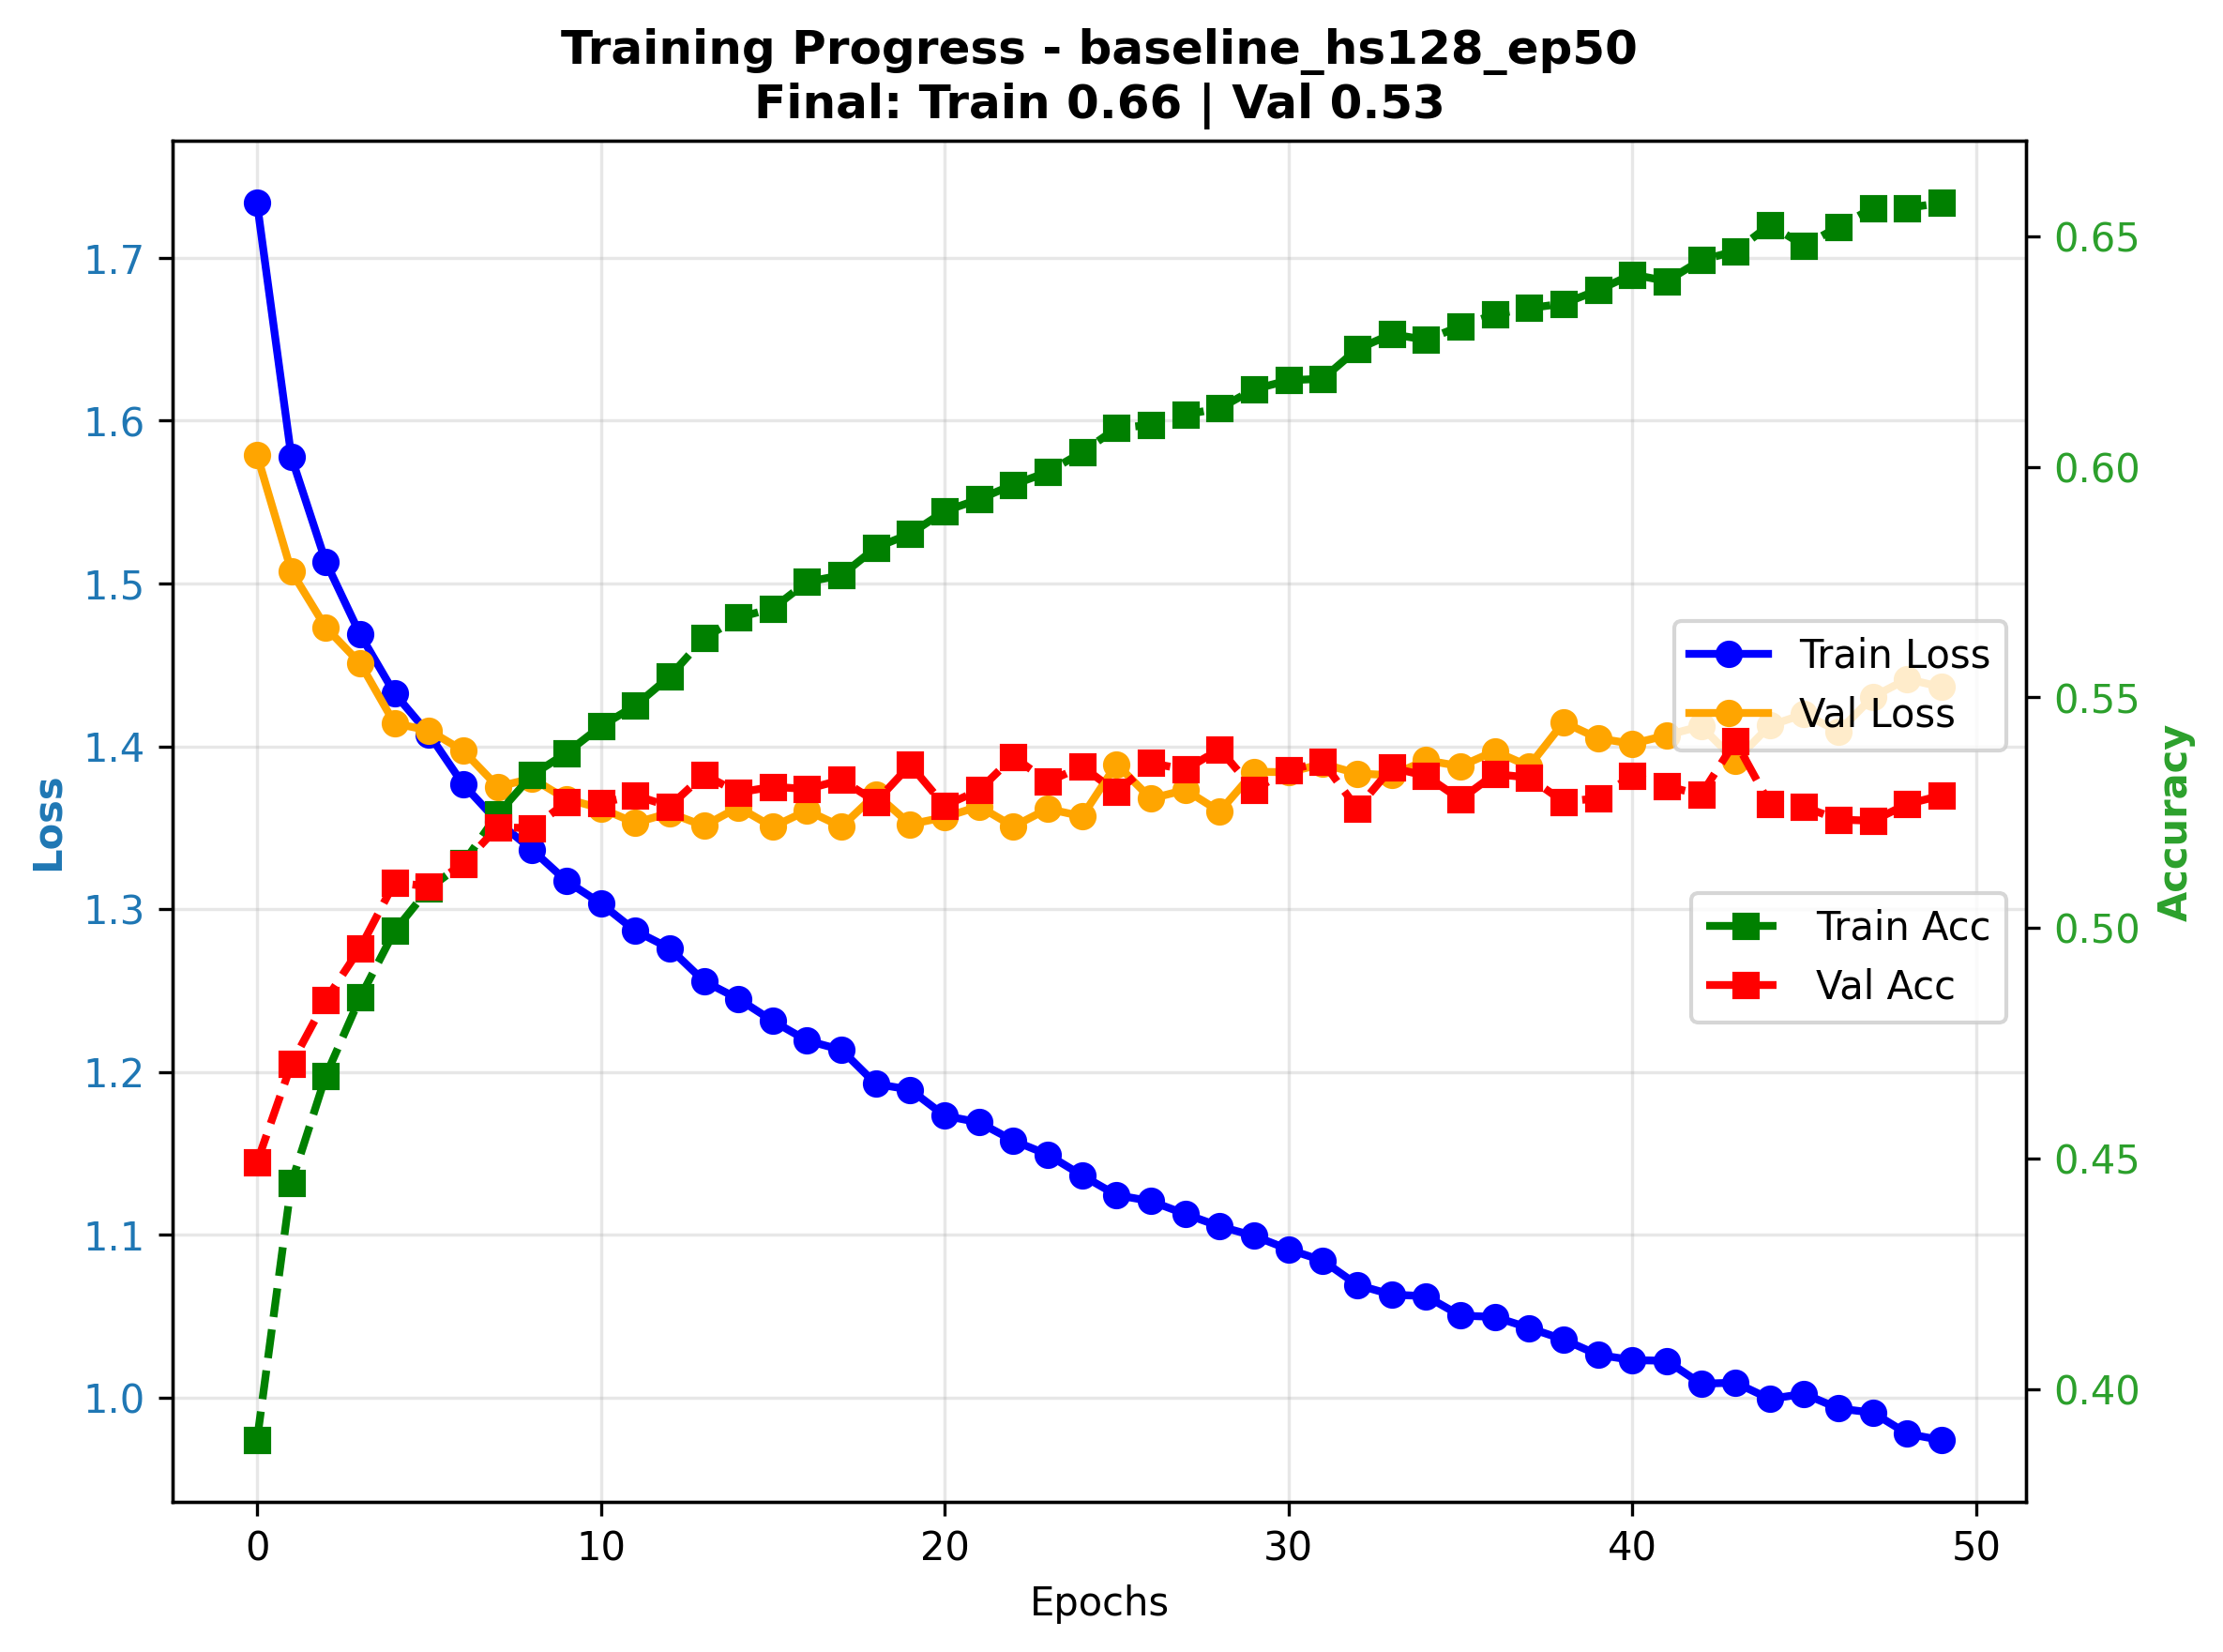
\includegraphics[width=\textwidth]{../plots/mlp/cifar10/hs128_ep50/baseline_hs128_ep50_training_curves.png}
            {\scriptsize
            \begin{tabular}{lcc}
                \toprule
                & \textbf{Baseline} & \textbf{Coherence} \\
                \midrule
                Final Test Loss & 1.44 & 2.31 \\
                Final Test Accuracy & 0.52 & \textbf{\textcolor{red}{0.51}} \\
                Best Epoch & 43 & \textbf{\textcolor{red}{24}} \\
                Best Val Accuracy & 0.54 & 0.53 \\
                \bottomrule
            \end{tabular}
            }

			\begin{itemize}
				\item A similar result is observed for MNIST, with better accuracy, but not for Fashion MNIST (see Annex).
			\end{itemize}
			\vspace{0.05\textheight}
        \end{minipage}%
        \hfill
        \begin{minipage}[b]{0.48\textwidth}
            \centering
            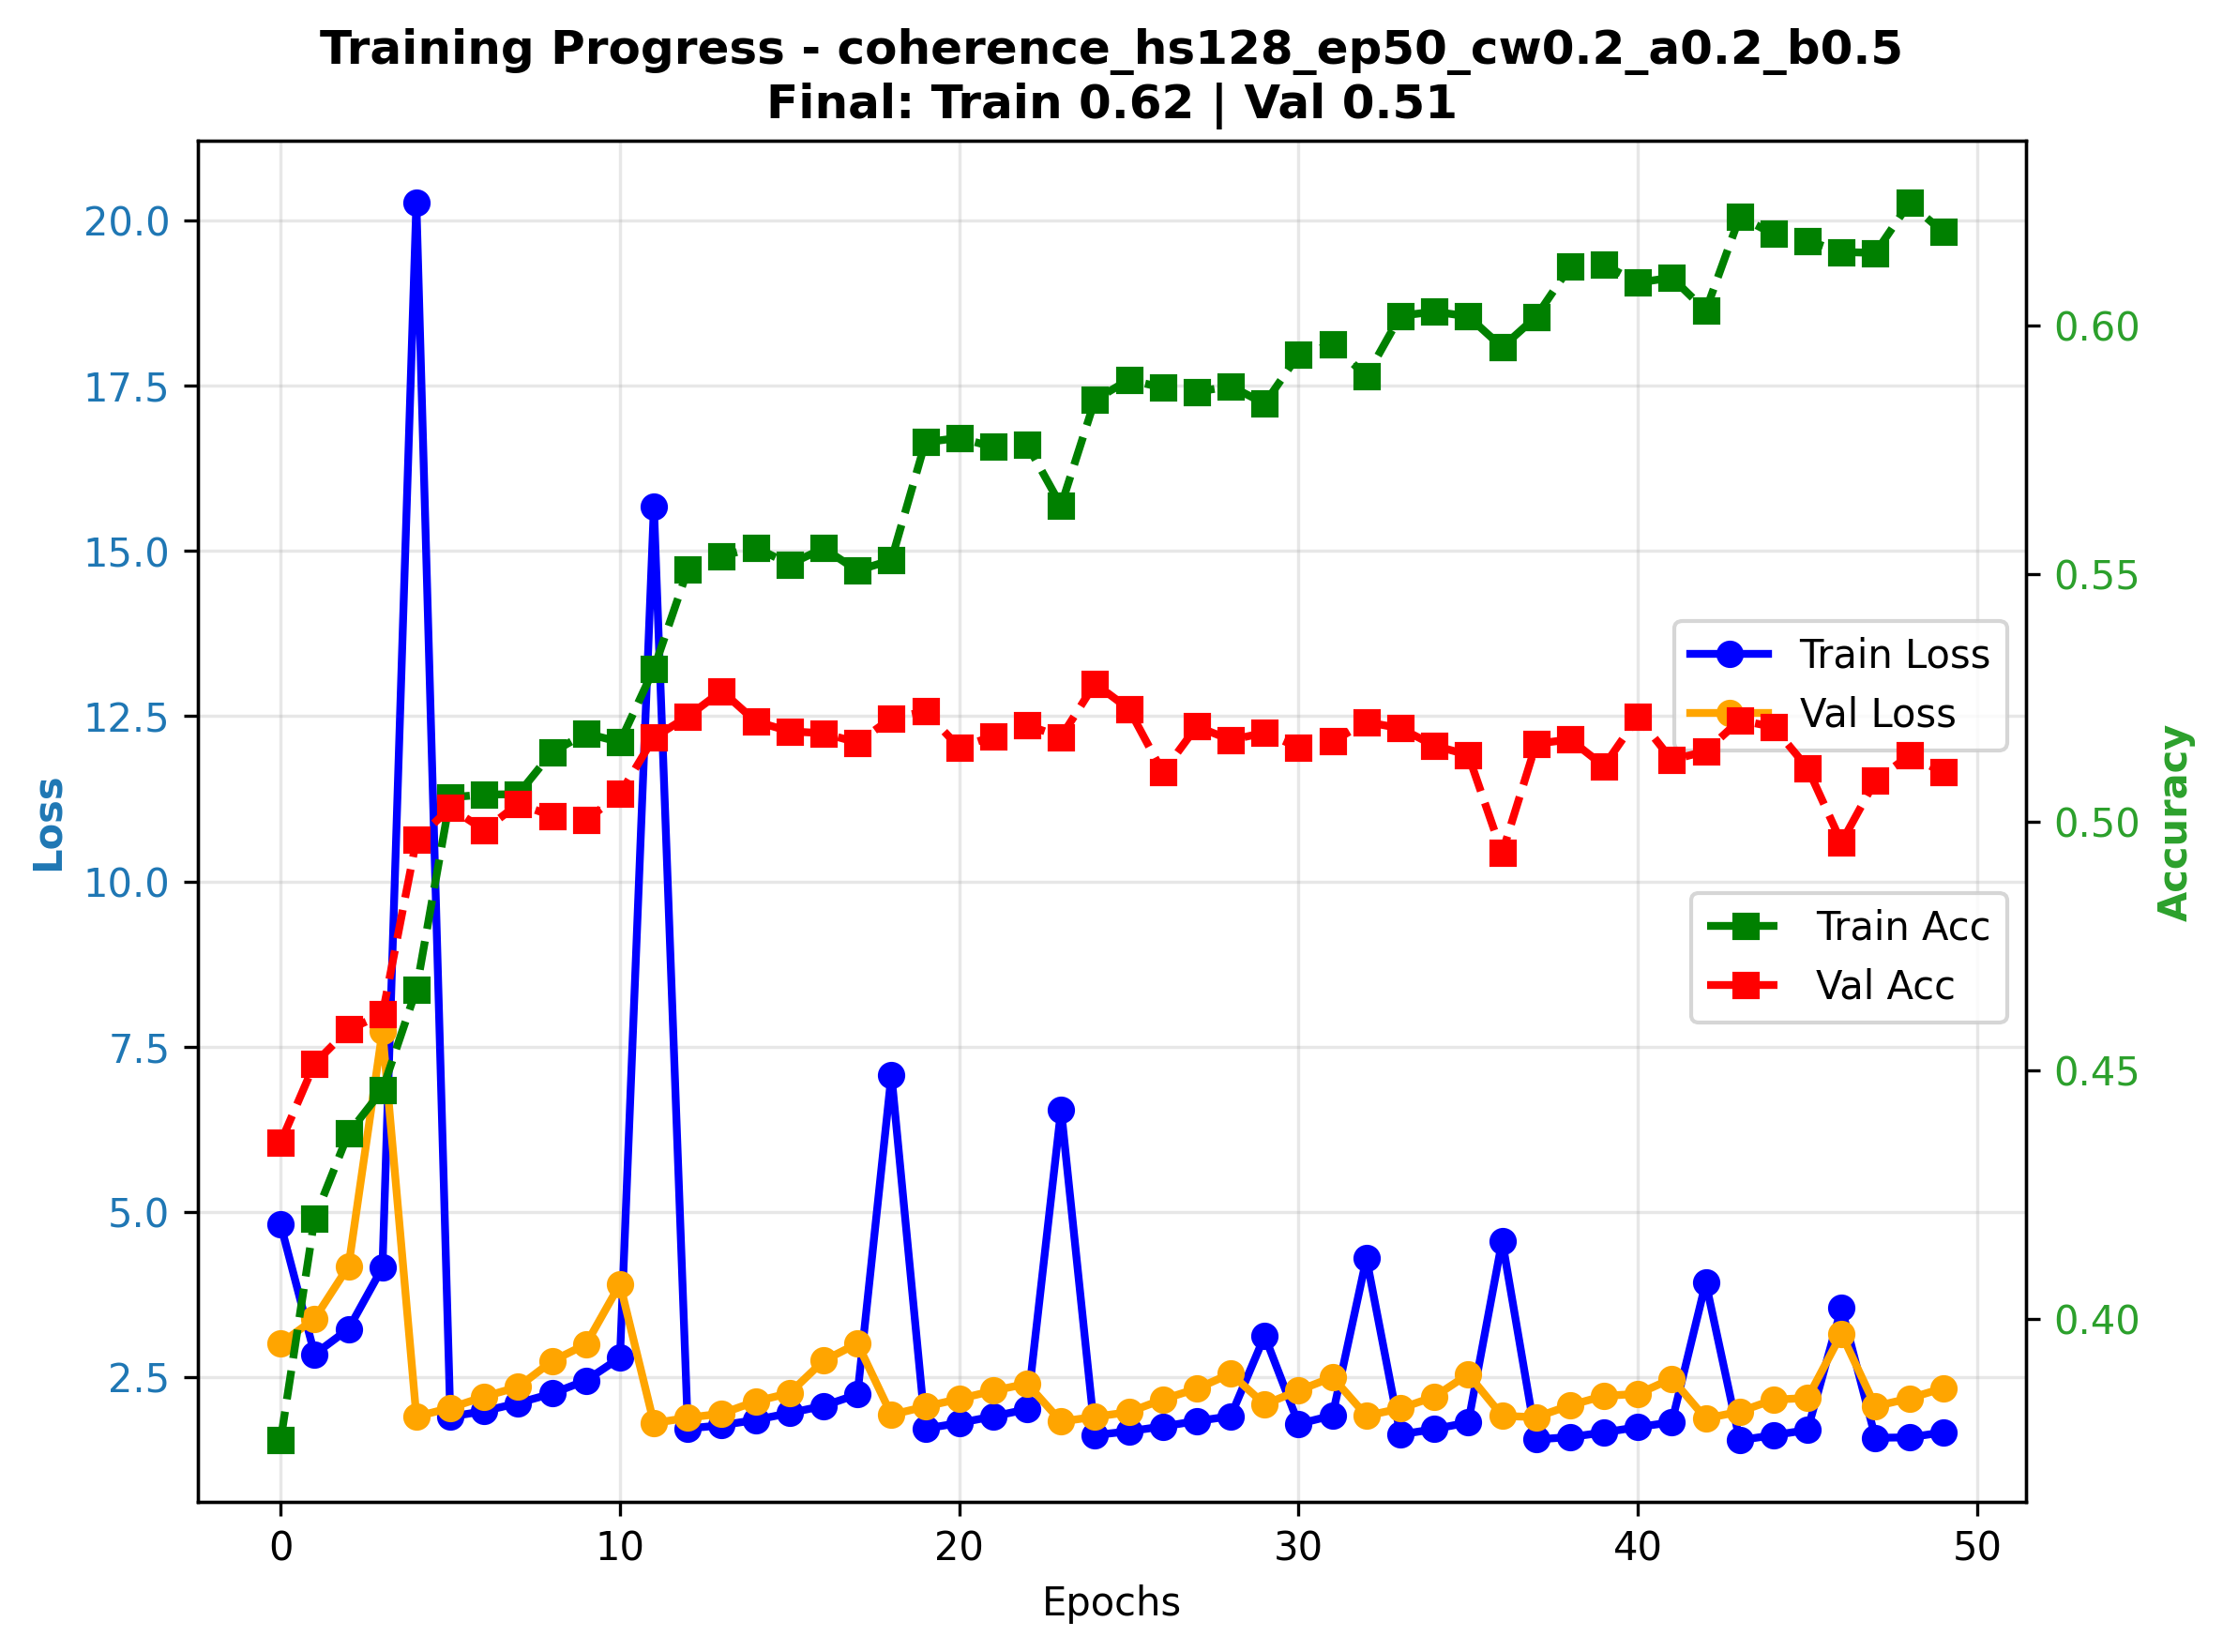
\includegraphics[width=\textwidth,height=0.48\textheight,keepaspectratio]{../plots/mlp/cifar10/hs128_ep50/coherence_hs128_ep50_cw0.2_a0.2_b0.5_training_curves.png} \\
            \vspace{0.5em}
            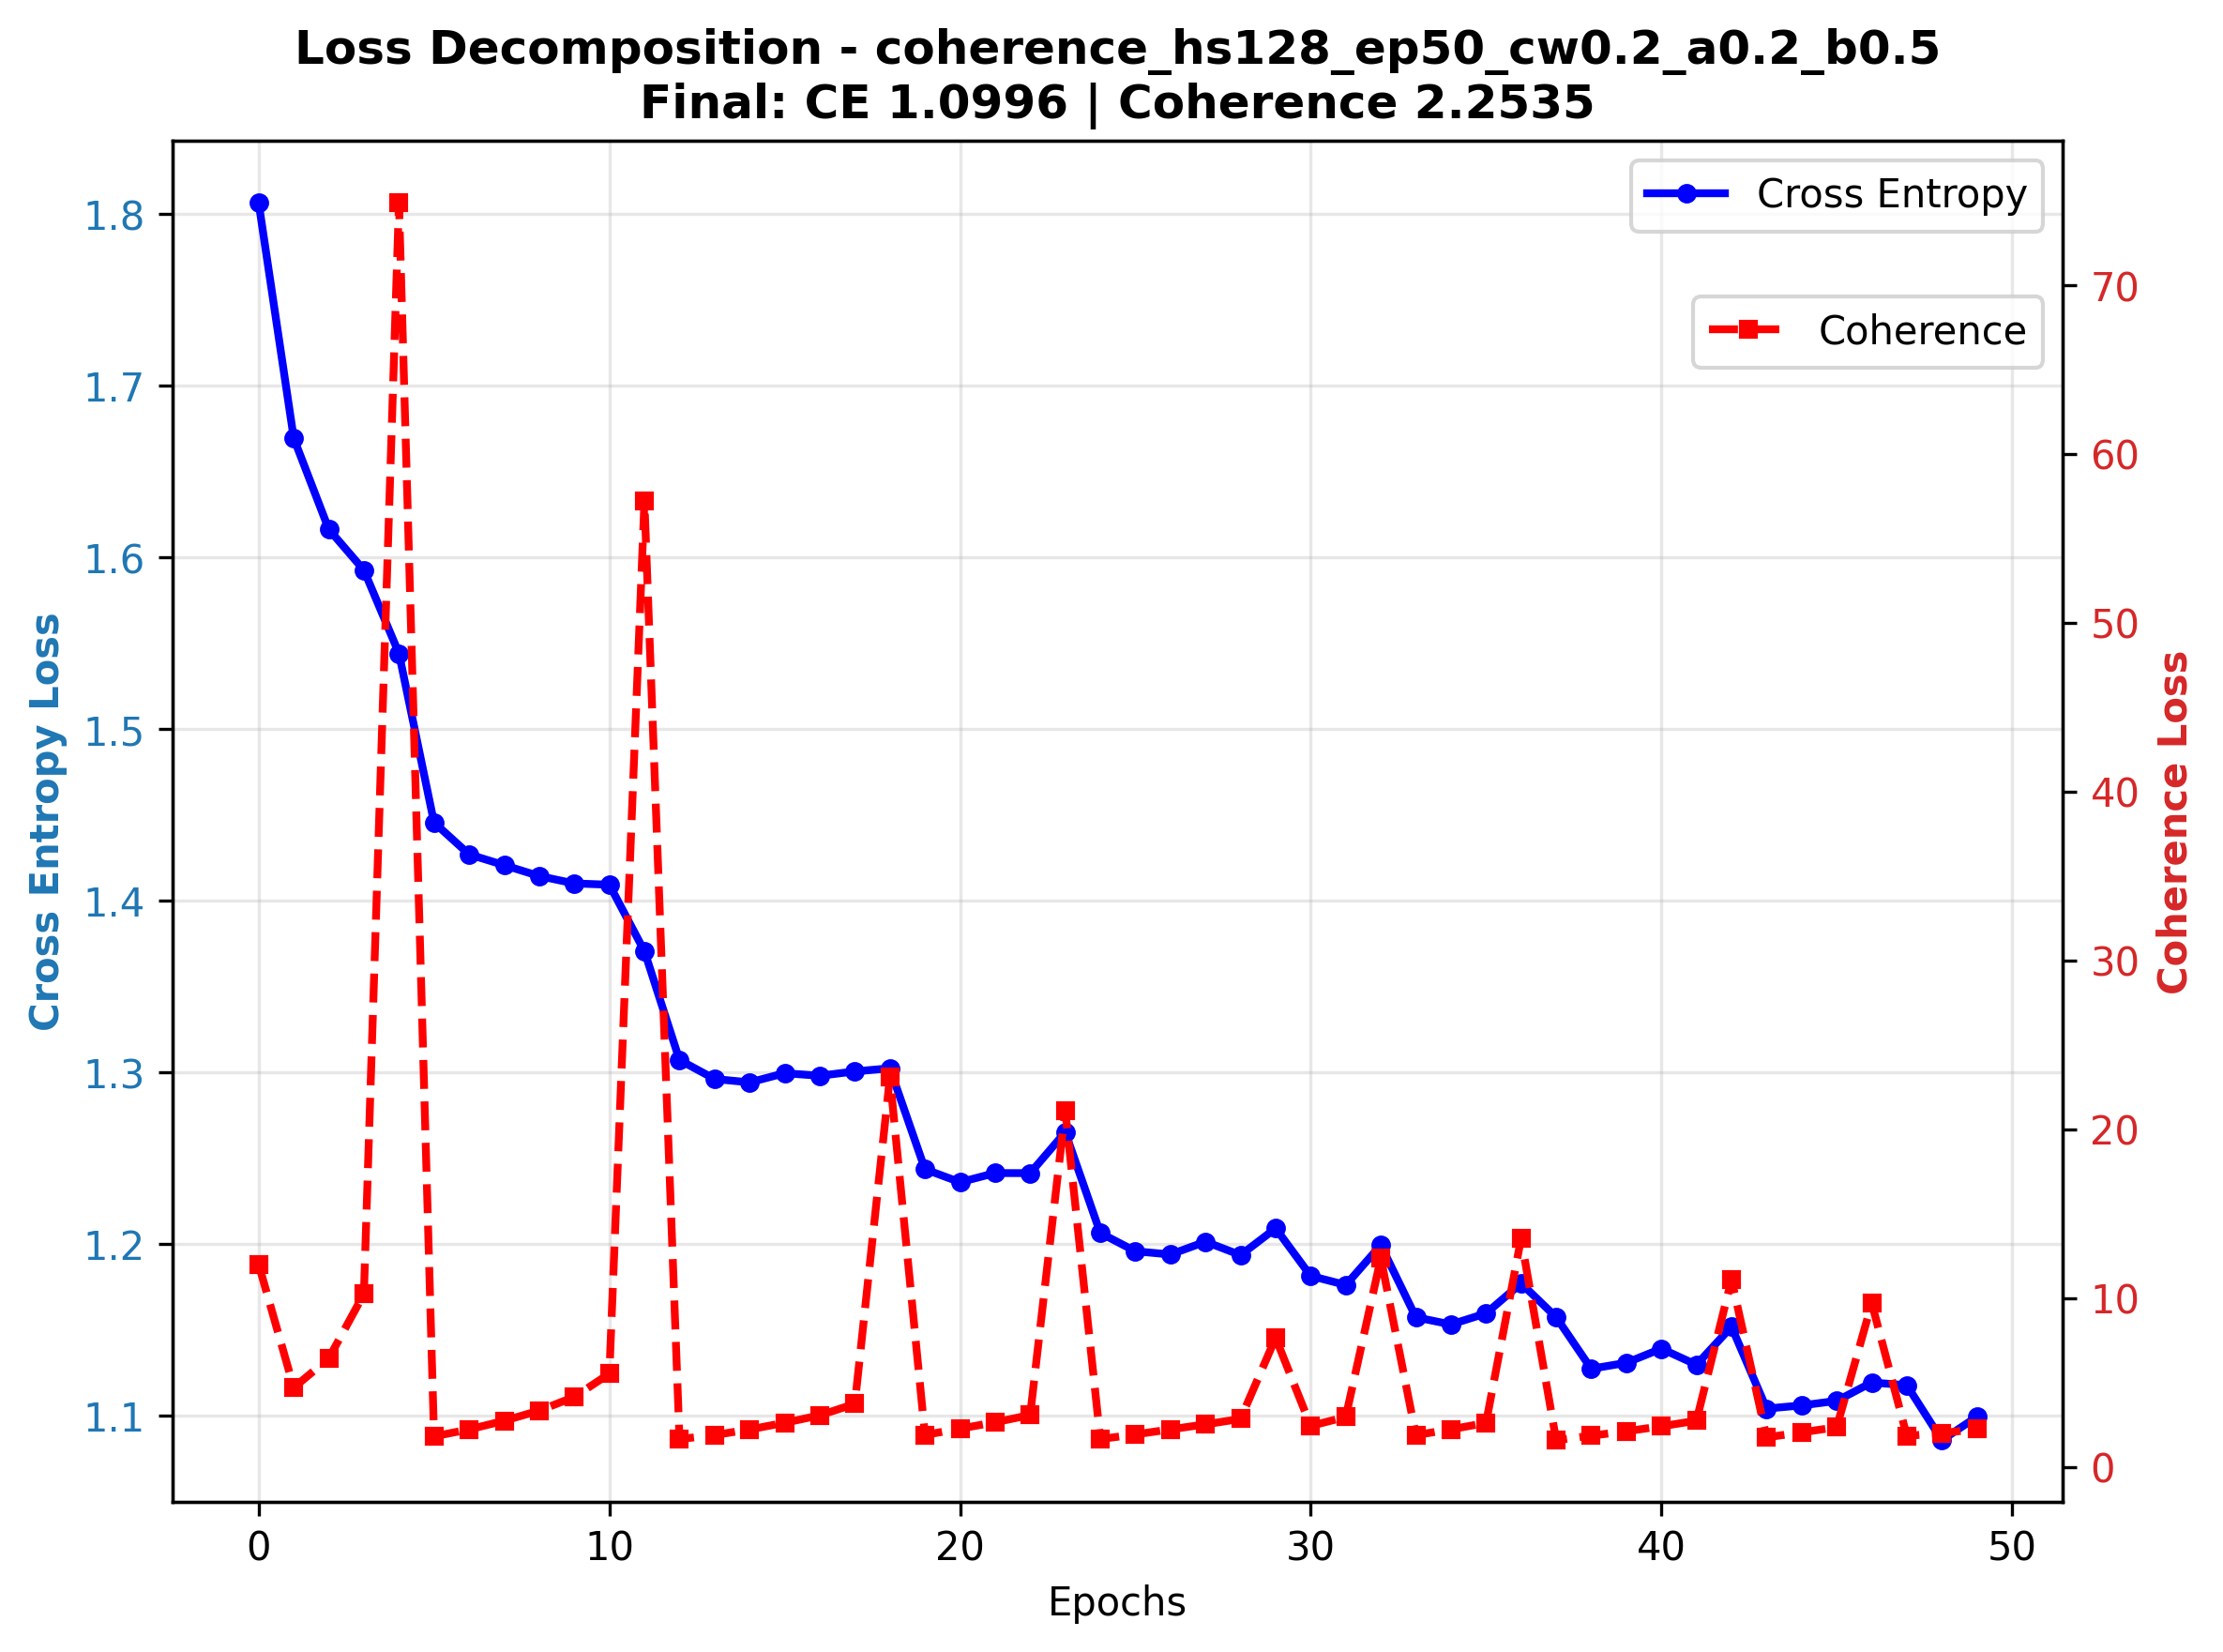
\includegraphics[width=\textwidth,height=0.48\textheight,keepaspectratio]{../plots/mlp/cifar10/hs128_ep50/coherence_hs128_ep50_cw0.2_a0.2_b0.5_loss_decomposition.png}
        \end{minipage}
    \end{figure}

\end{frame}
%--------------------------------------------------------------------------------------
\begin{frame}{Implementation Results: CIFAR10}
    \begin{figure}[H]
        \centering
        % 2x1 subfigures (vertical stack, reduced height and spacing)
        \begin{minipage}[b]{\textwidth}
            \centering
            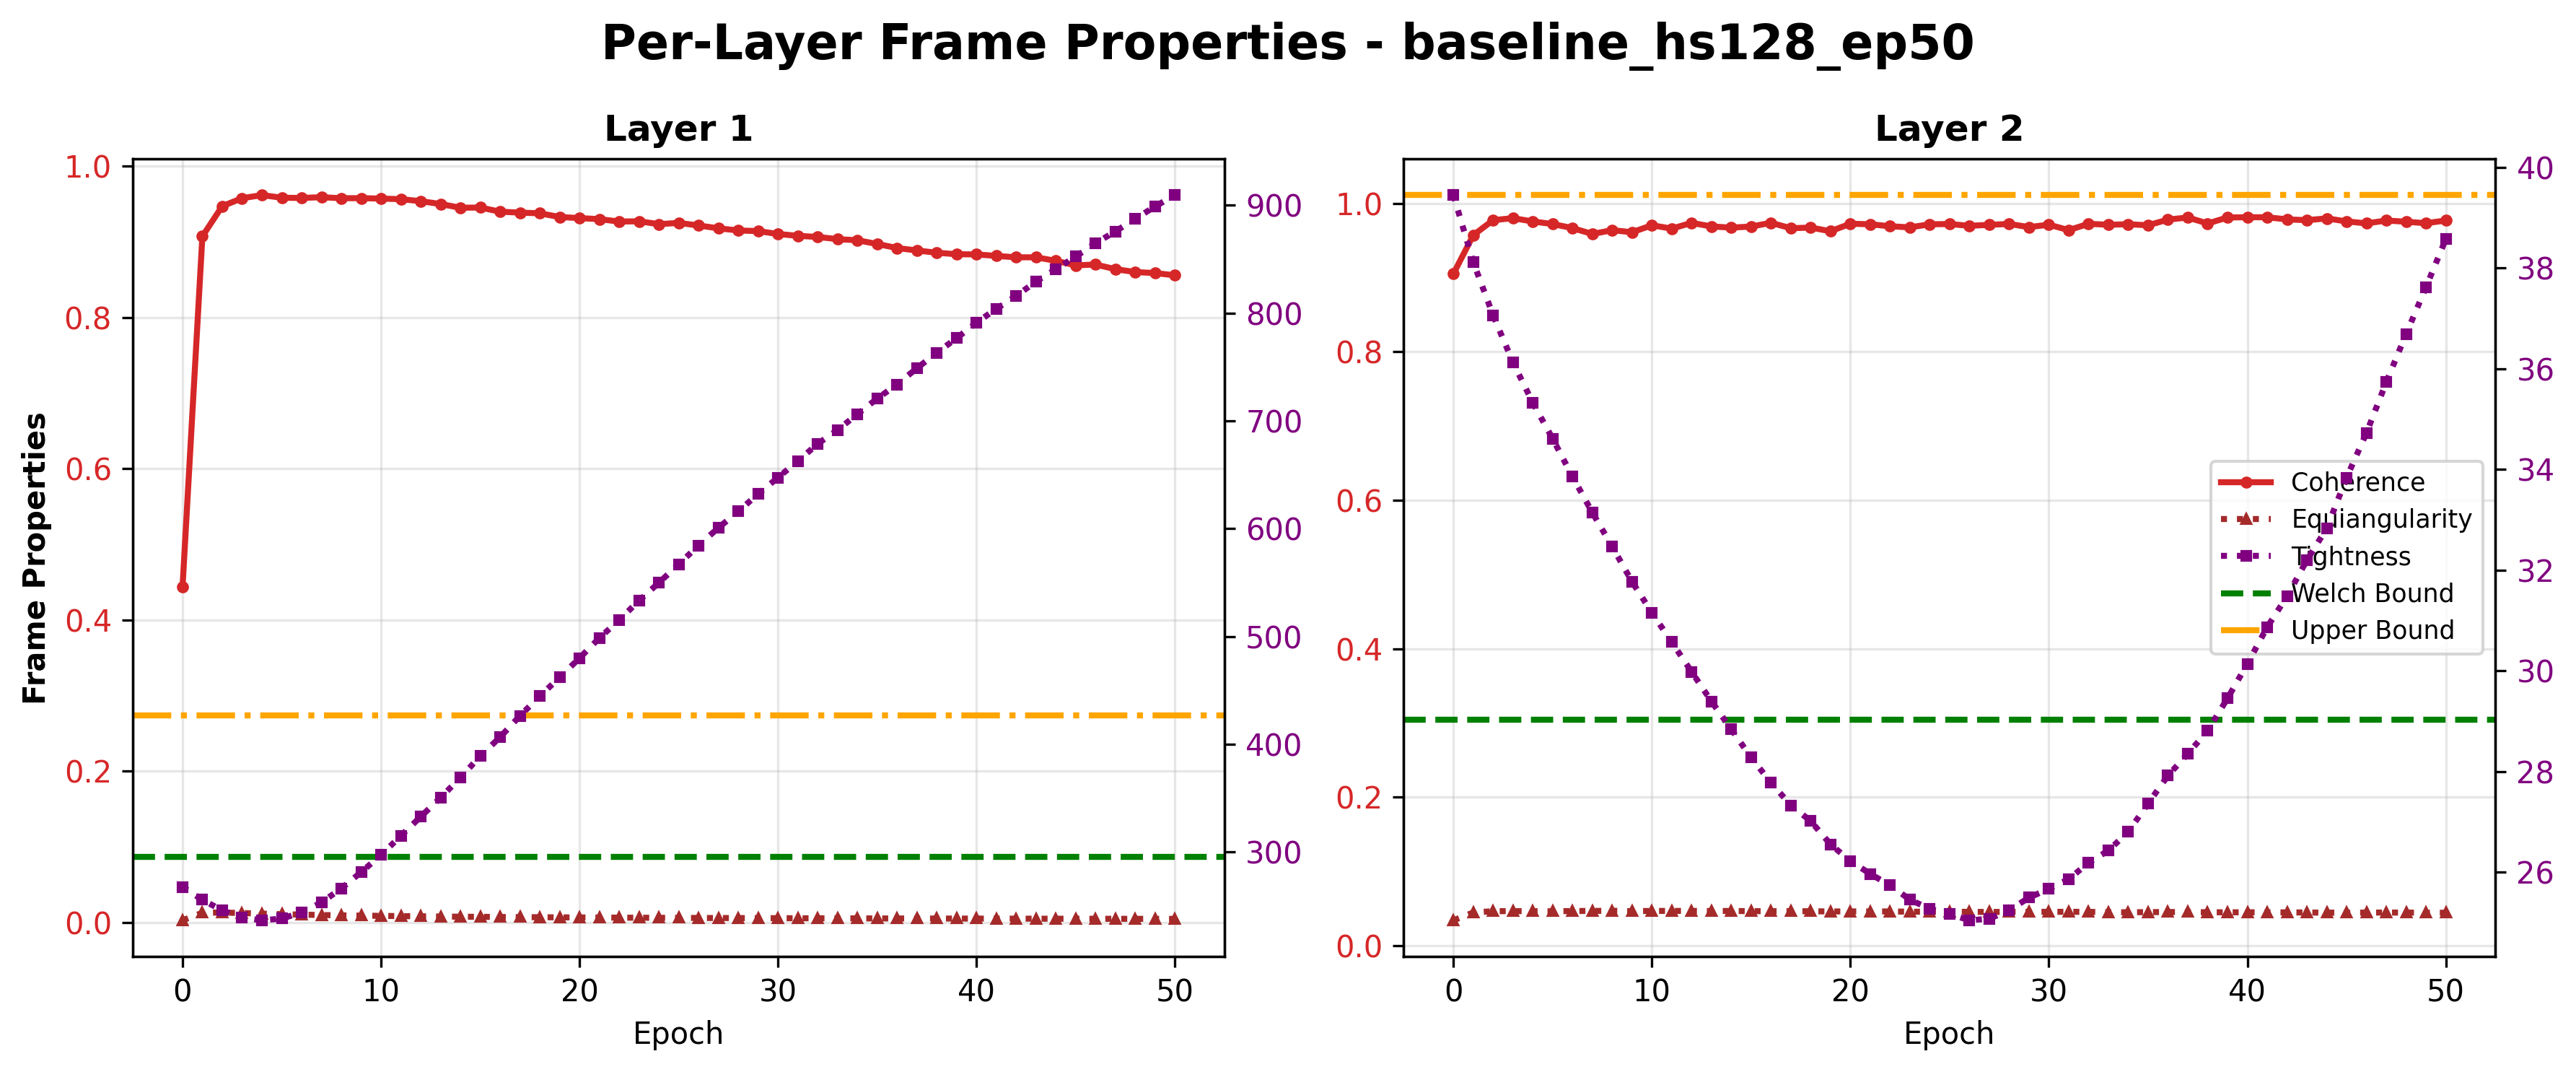
\includegraphics[width=\textwidth,height=0.45\textheight,keepaspectratio]{../plots/mlp/cifar10/hs128_ep50/baseline_hs128_ep50_coherence_analysis.png}
        \end{minipage}\\[0.1em]
        \begin{minipage}[b]{\textwidth}
            \centering
            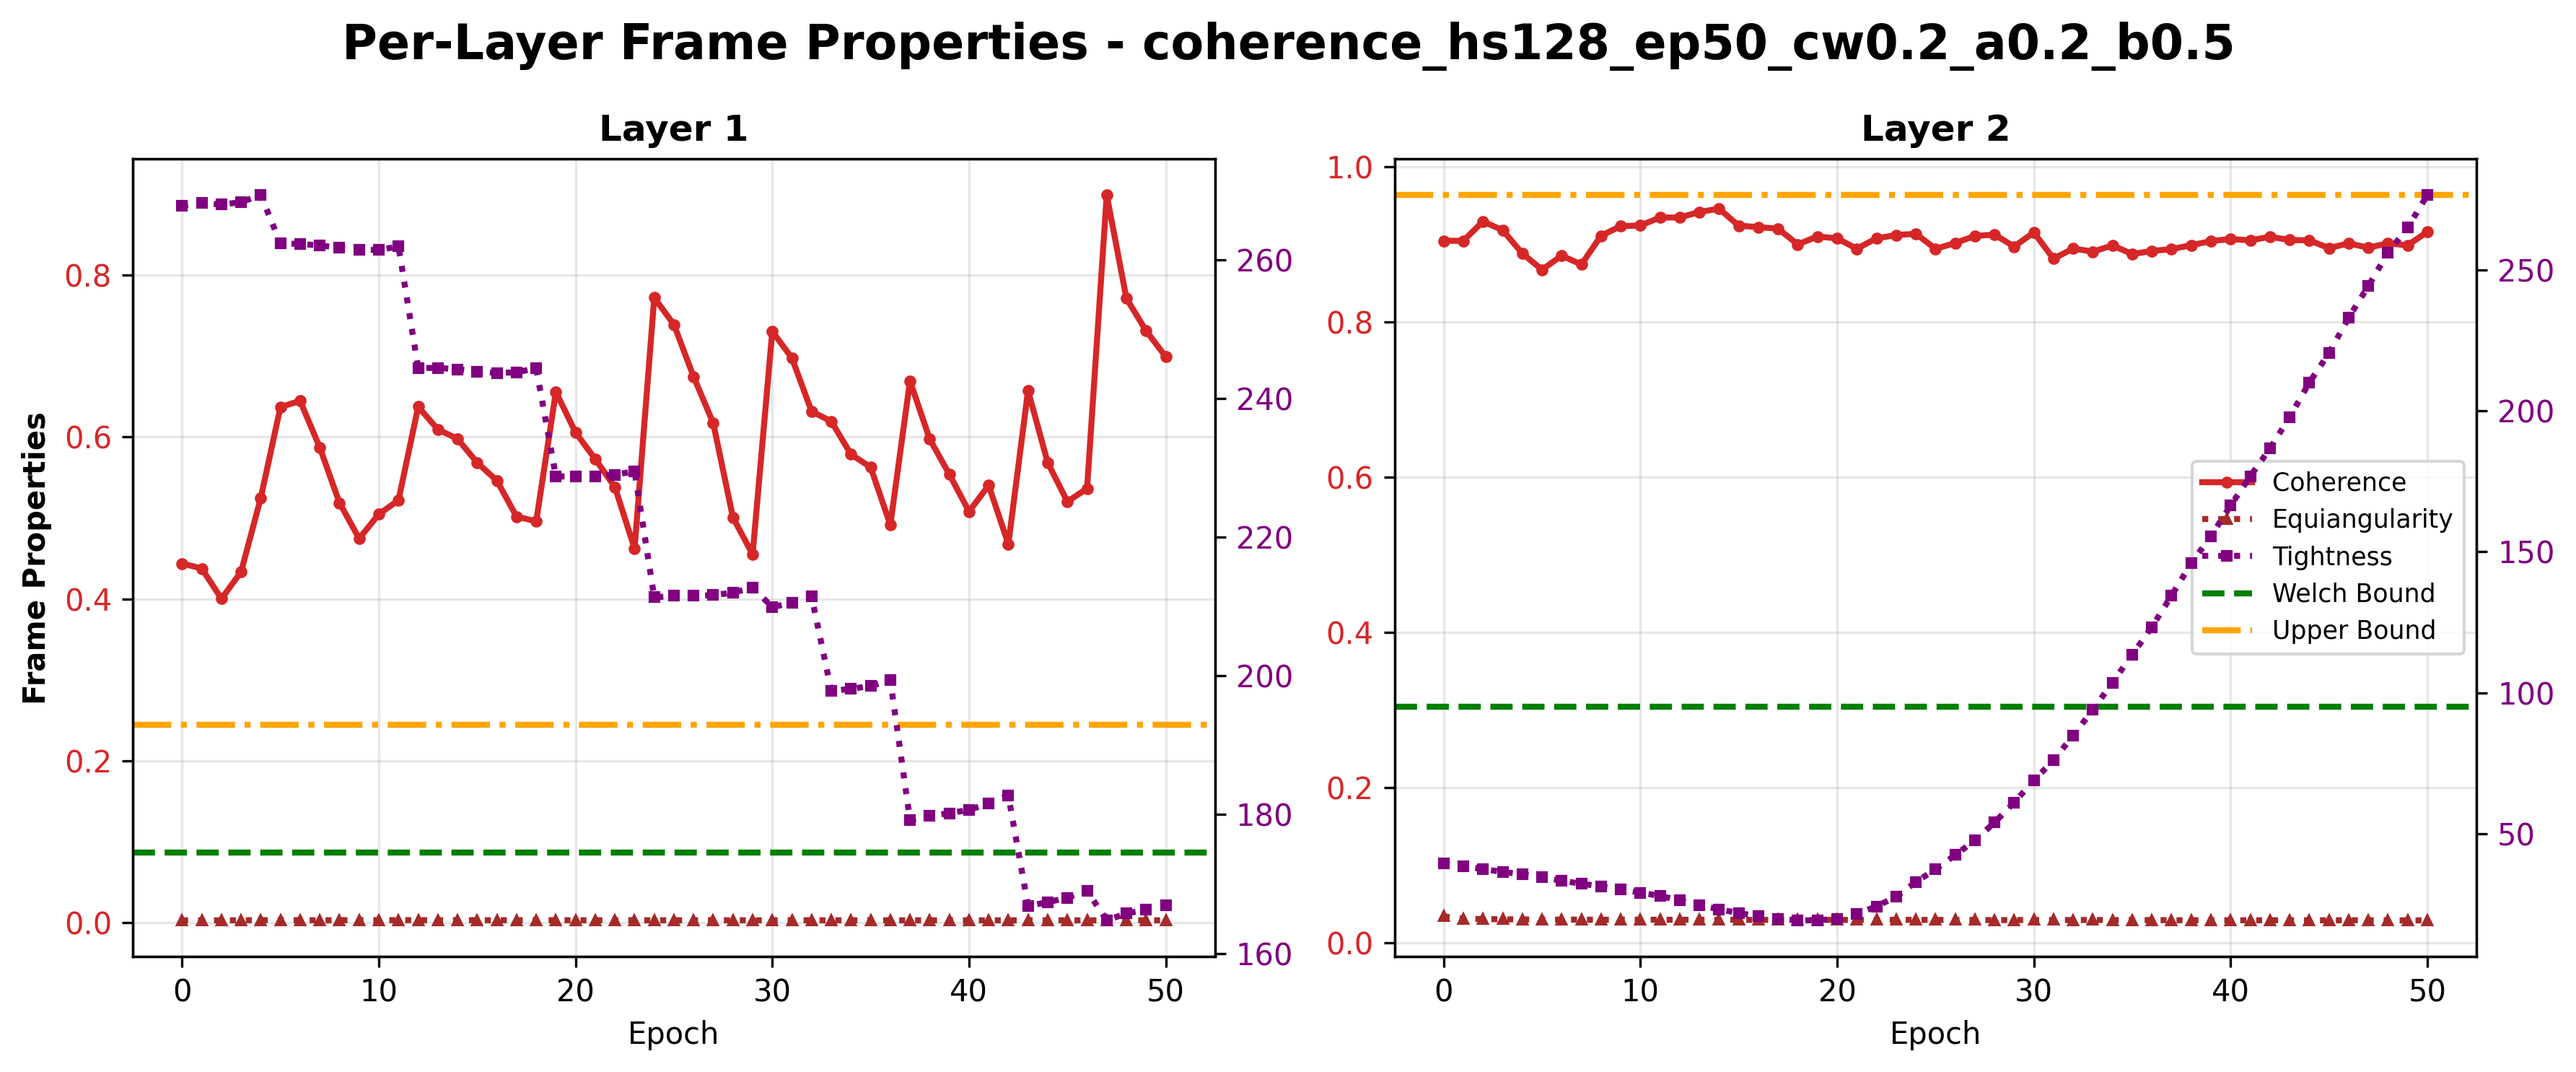
\includegraphics[width=\textwidth,height=0.45\textheight,keepaspectratio]{../plots/mlp/cifar10/hs128_ep50/coherence_hs128_ep50_cw0.2_a0.2_b0.5_coherence_analysis.png}
        \end{minipage}
    \end{figure}
\end{frame}
%--------------------------------------------------------------------------------------
\begin{frame}{Implementation Results: CIFAR10}
    \begin{figure}[H]
        \centering
        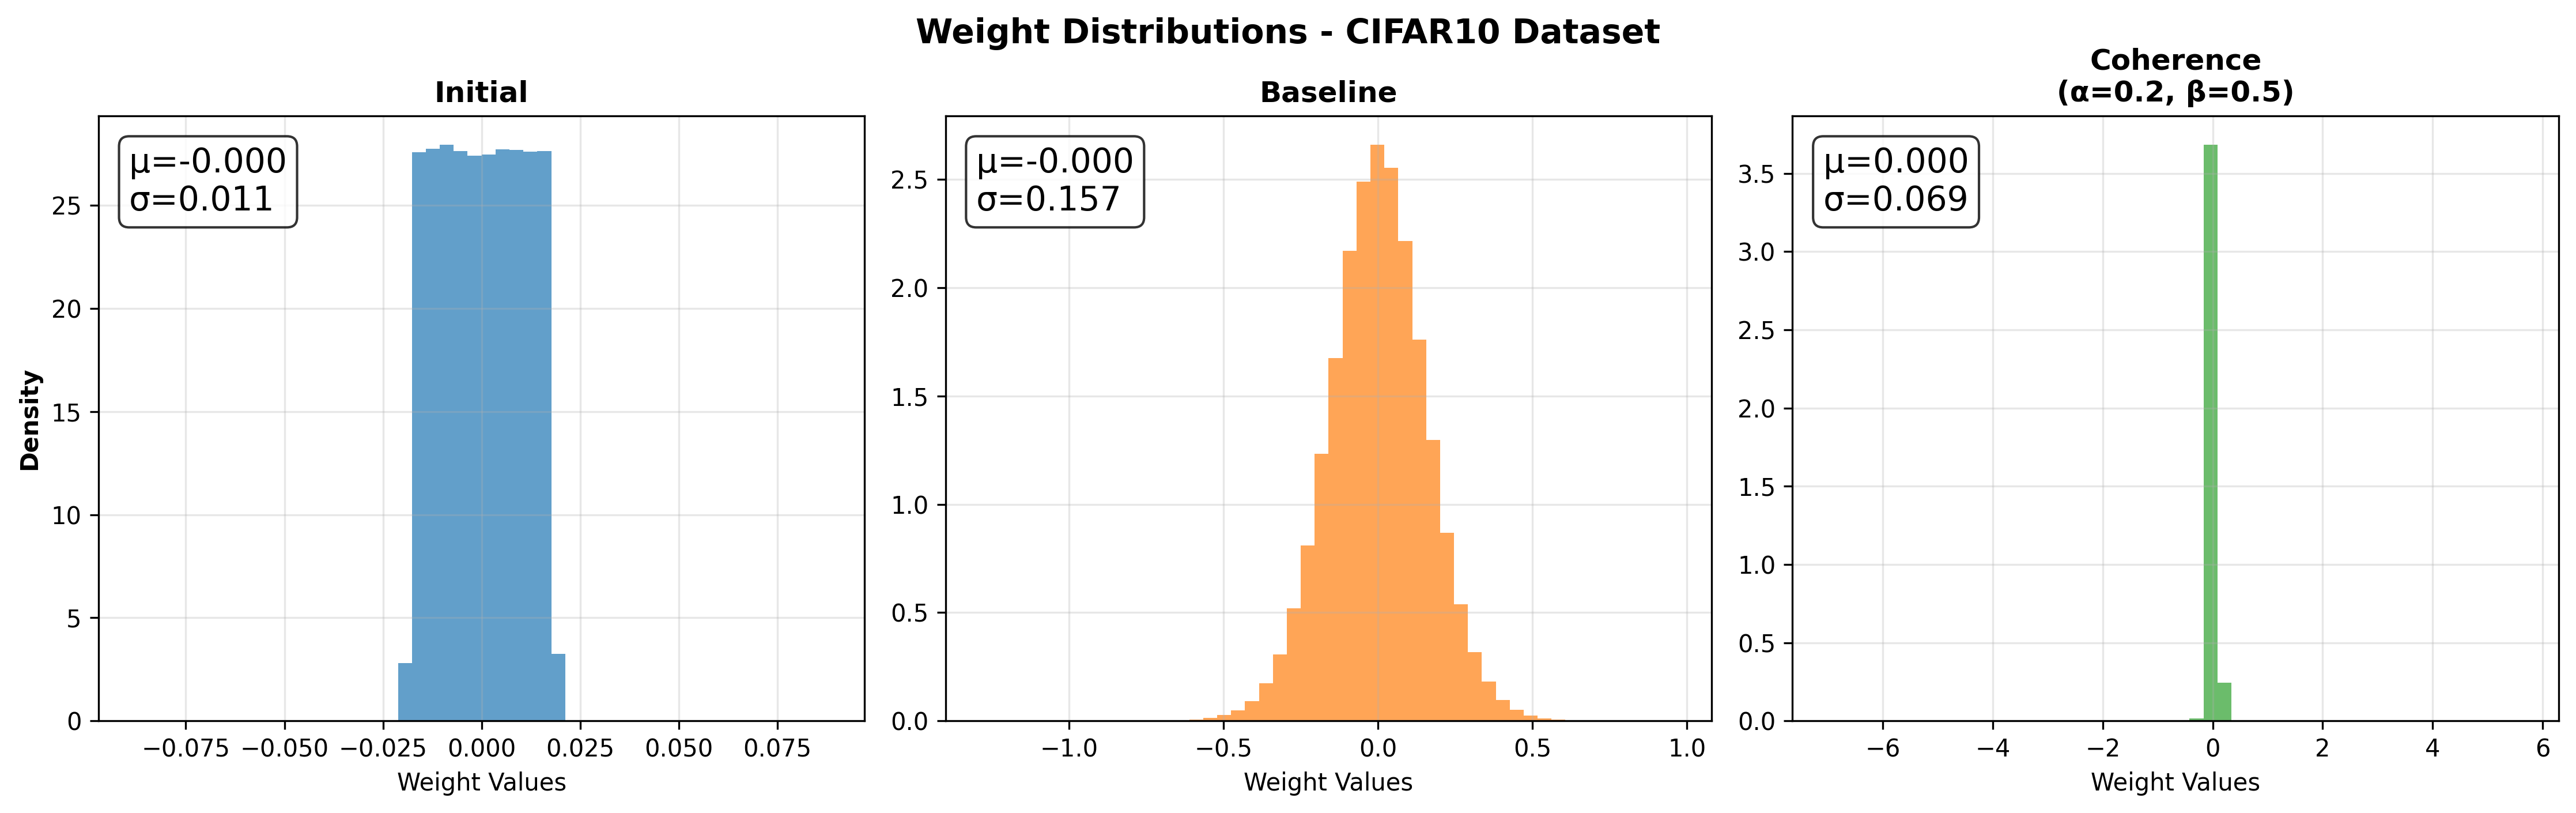
\includegraphics[width=\textwidth]{../plots/mlp/cifar10/hs128_ep50/weights_distribution_baseline.png}
    \end{figure}

	\textbf{Remark:} Regularization = Coherence + Equiangularity + Tightness.

	\textbf{Obs:} The minimum coherence optimization slows down training.
\end{frame}
%--------------------------------------------------------------------------------------
\begin{frame}{Implementation Results: MNIST}

    % 2-column figure: baseline (left), coherence model (right, stacked)
    
    \begin{figure}[H]
        \centering
        \begin{minipage}[b]{0.48\textwidth}
            \centering
            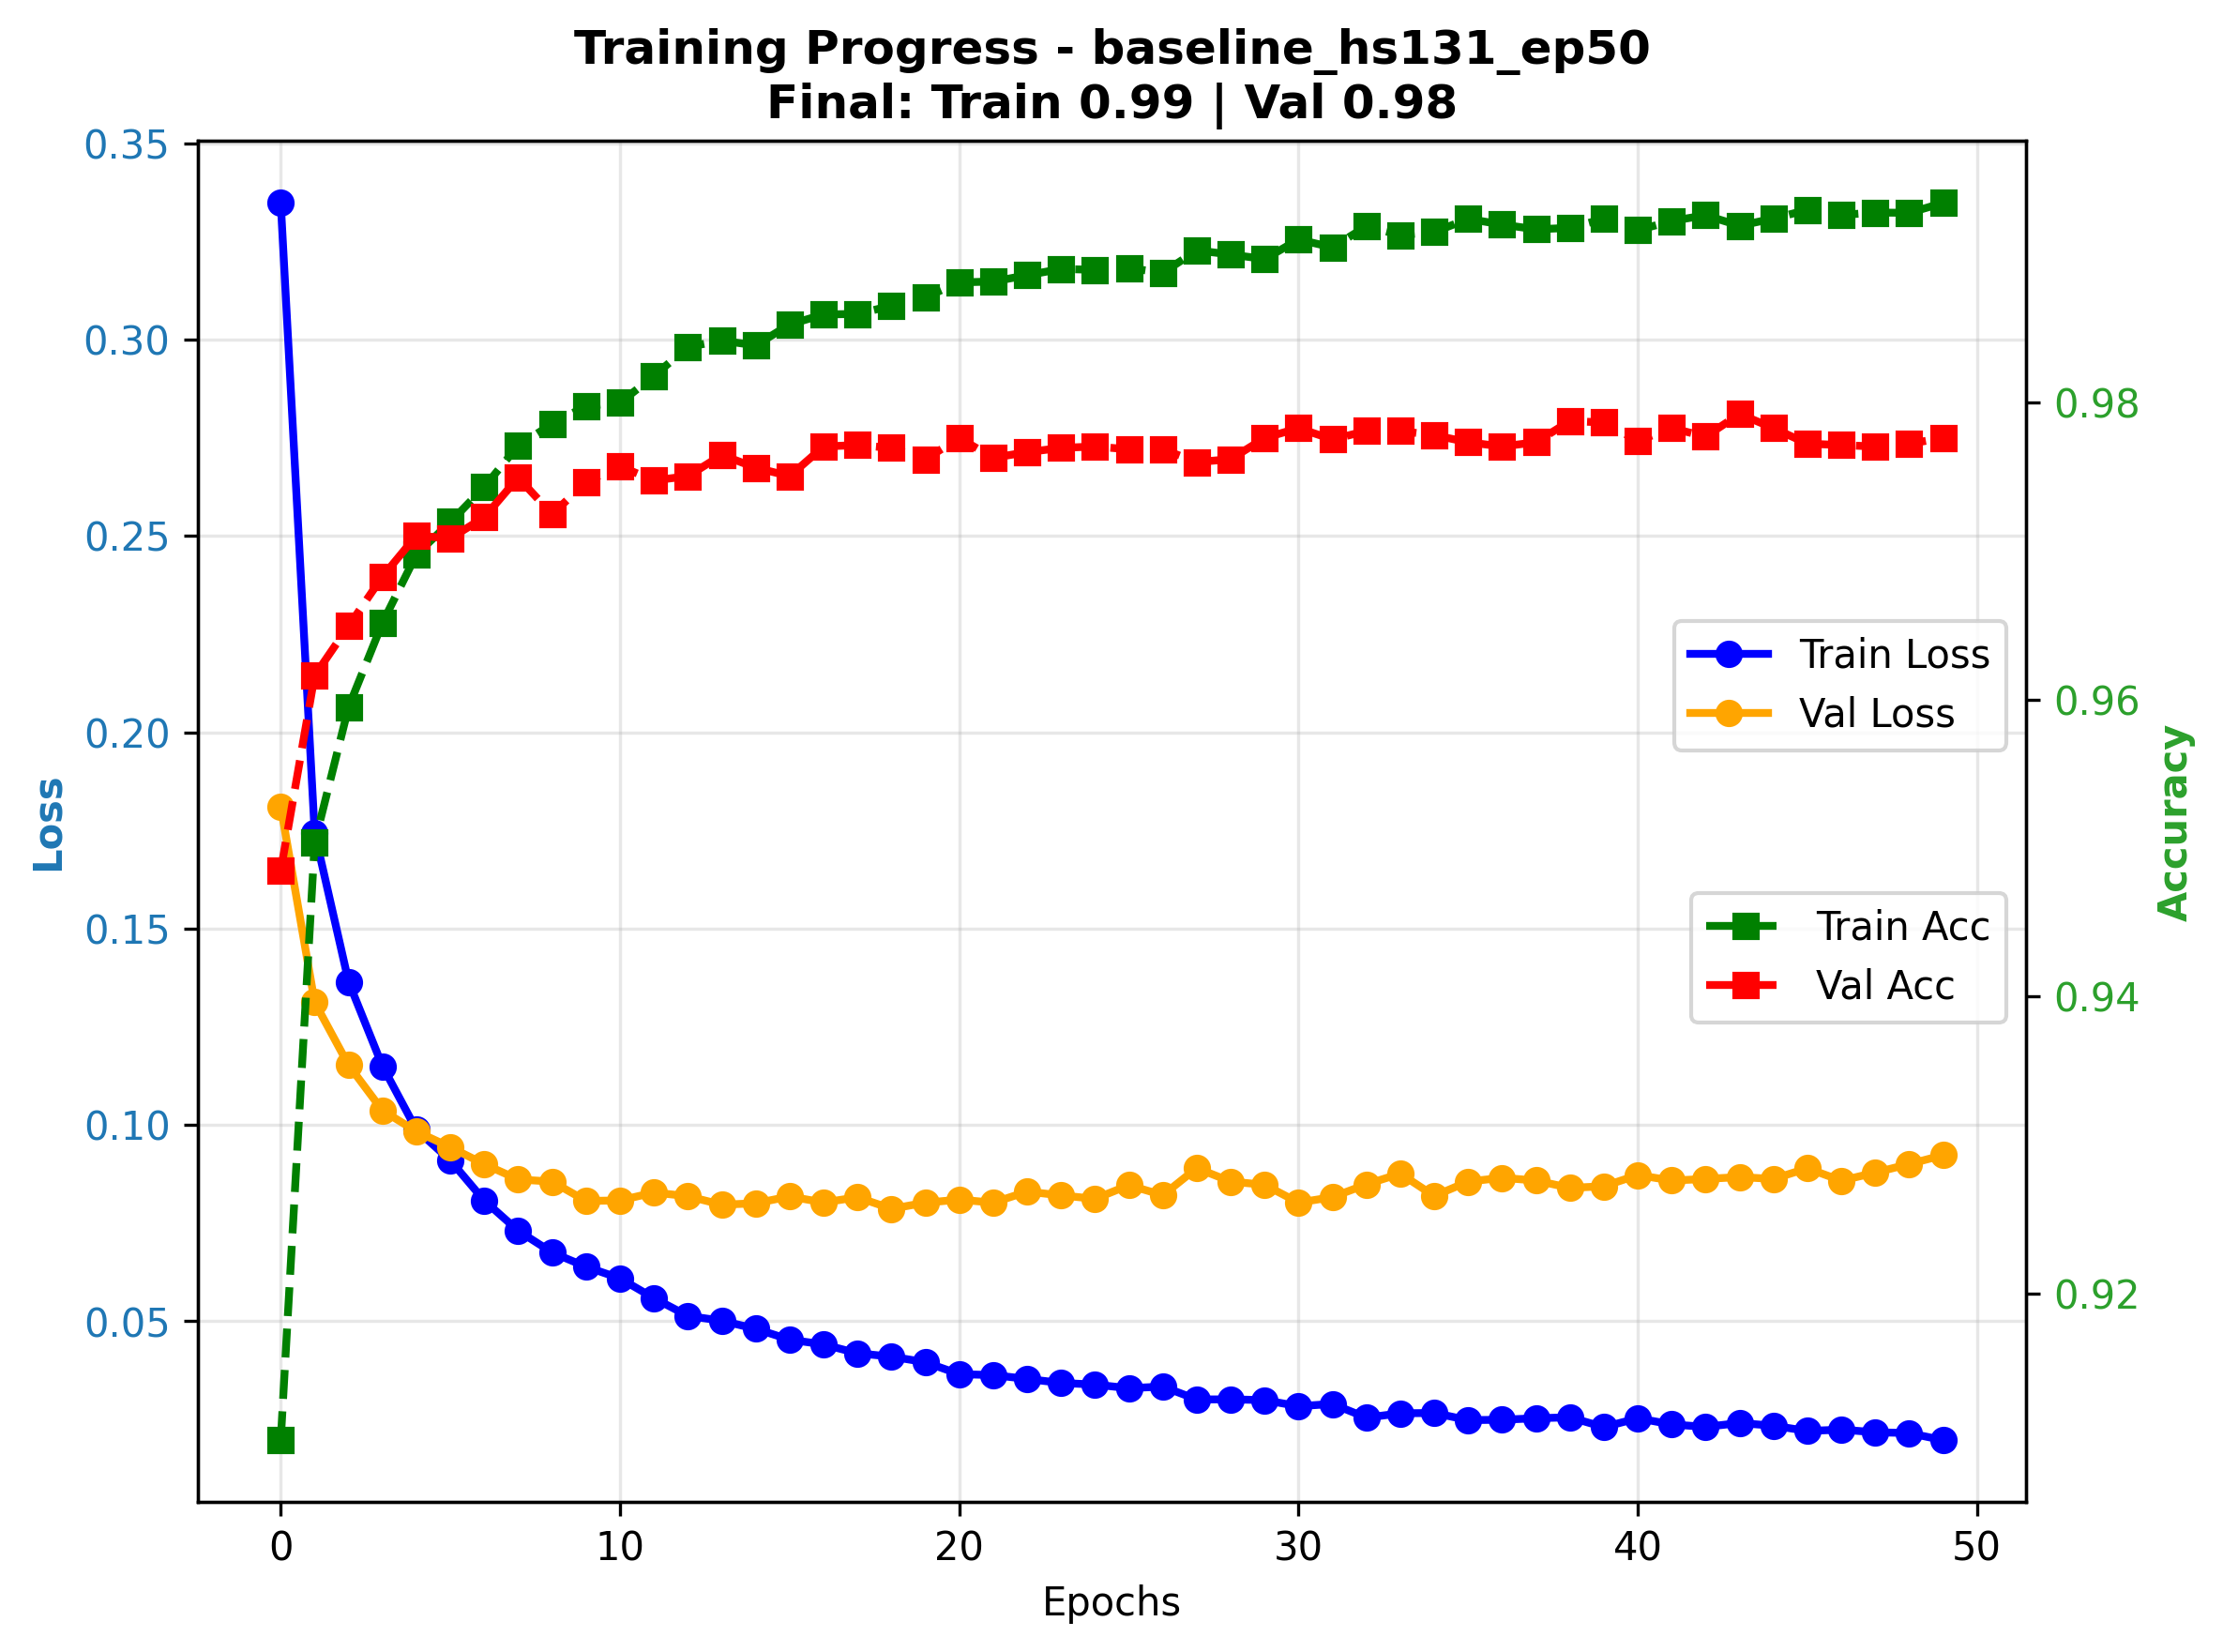
\includegraphics[width=\textwidth]{../plots/mlp/mnist/hs131_ep50/baseline_hs131_ep50_training_curves.png}
			\vspace{0.2\textheight}
            {\scriptsize
            \begin{tabular}{lcc}
                \toprule
                & \textbf{Baseline} & \textbf{Coherence} \\
                \midrule
                Final Test Loss & 0.08 & 0.94 \\
                Final Test Accuracy & 0.98 & \textbf{\textcolor{red}{0.97}} \\
                Best Epoch & 43 & \textbf{\textcolor{red}{38}} \\
                Best Val Accuracy & 0.98 & 0.97 \\
                \bottomrule
            \end{tabular}
            }
			\vspace{0.1\textheight}
        \end{minipage}%
        \hfill
        \begin{minipage}[b]{0.48\textwidth}
            \centering
            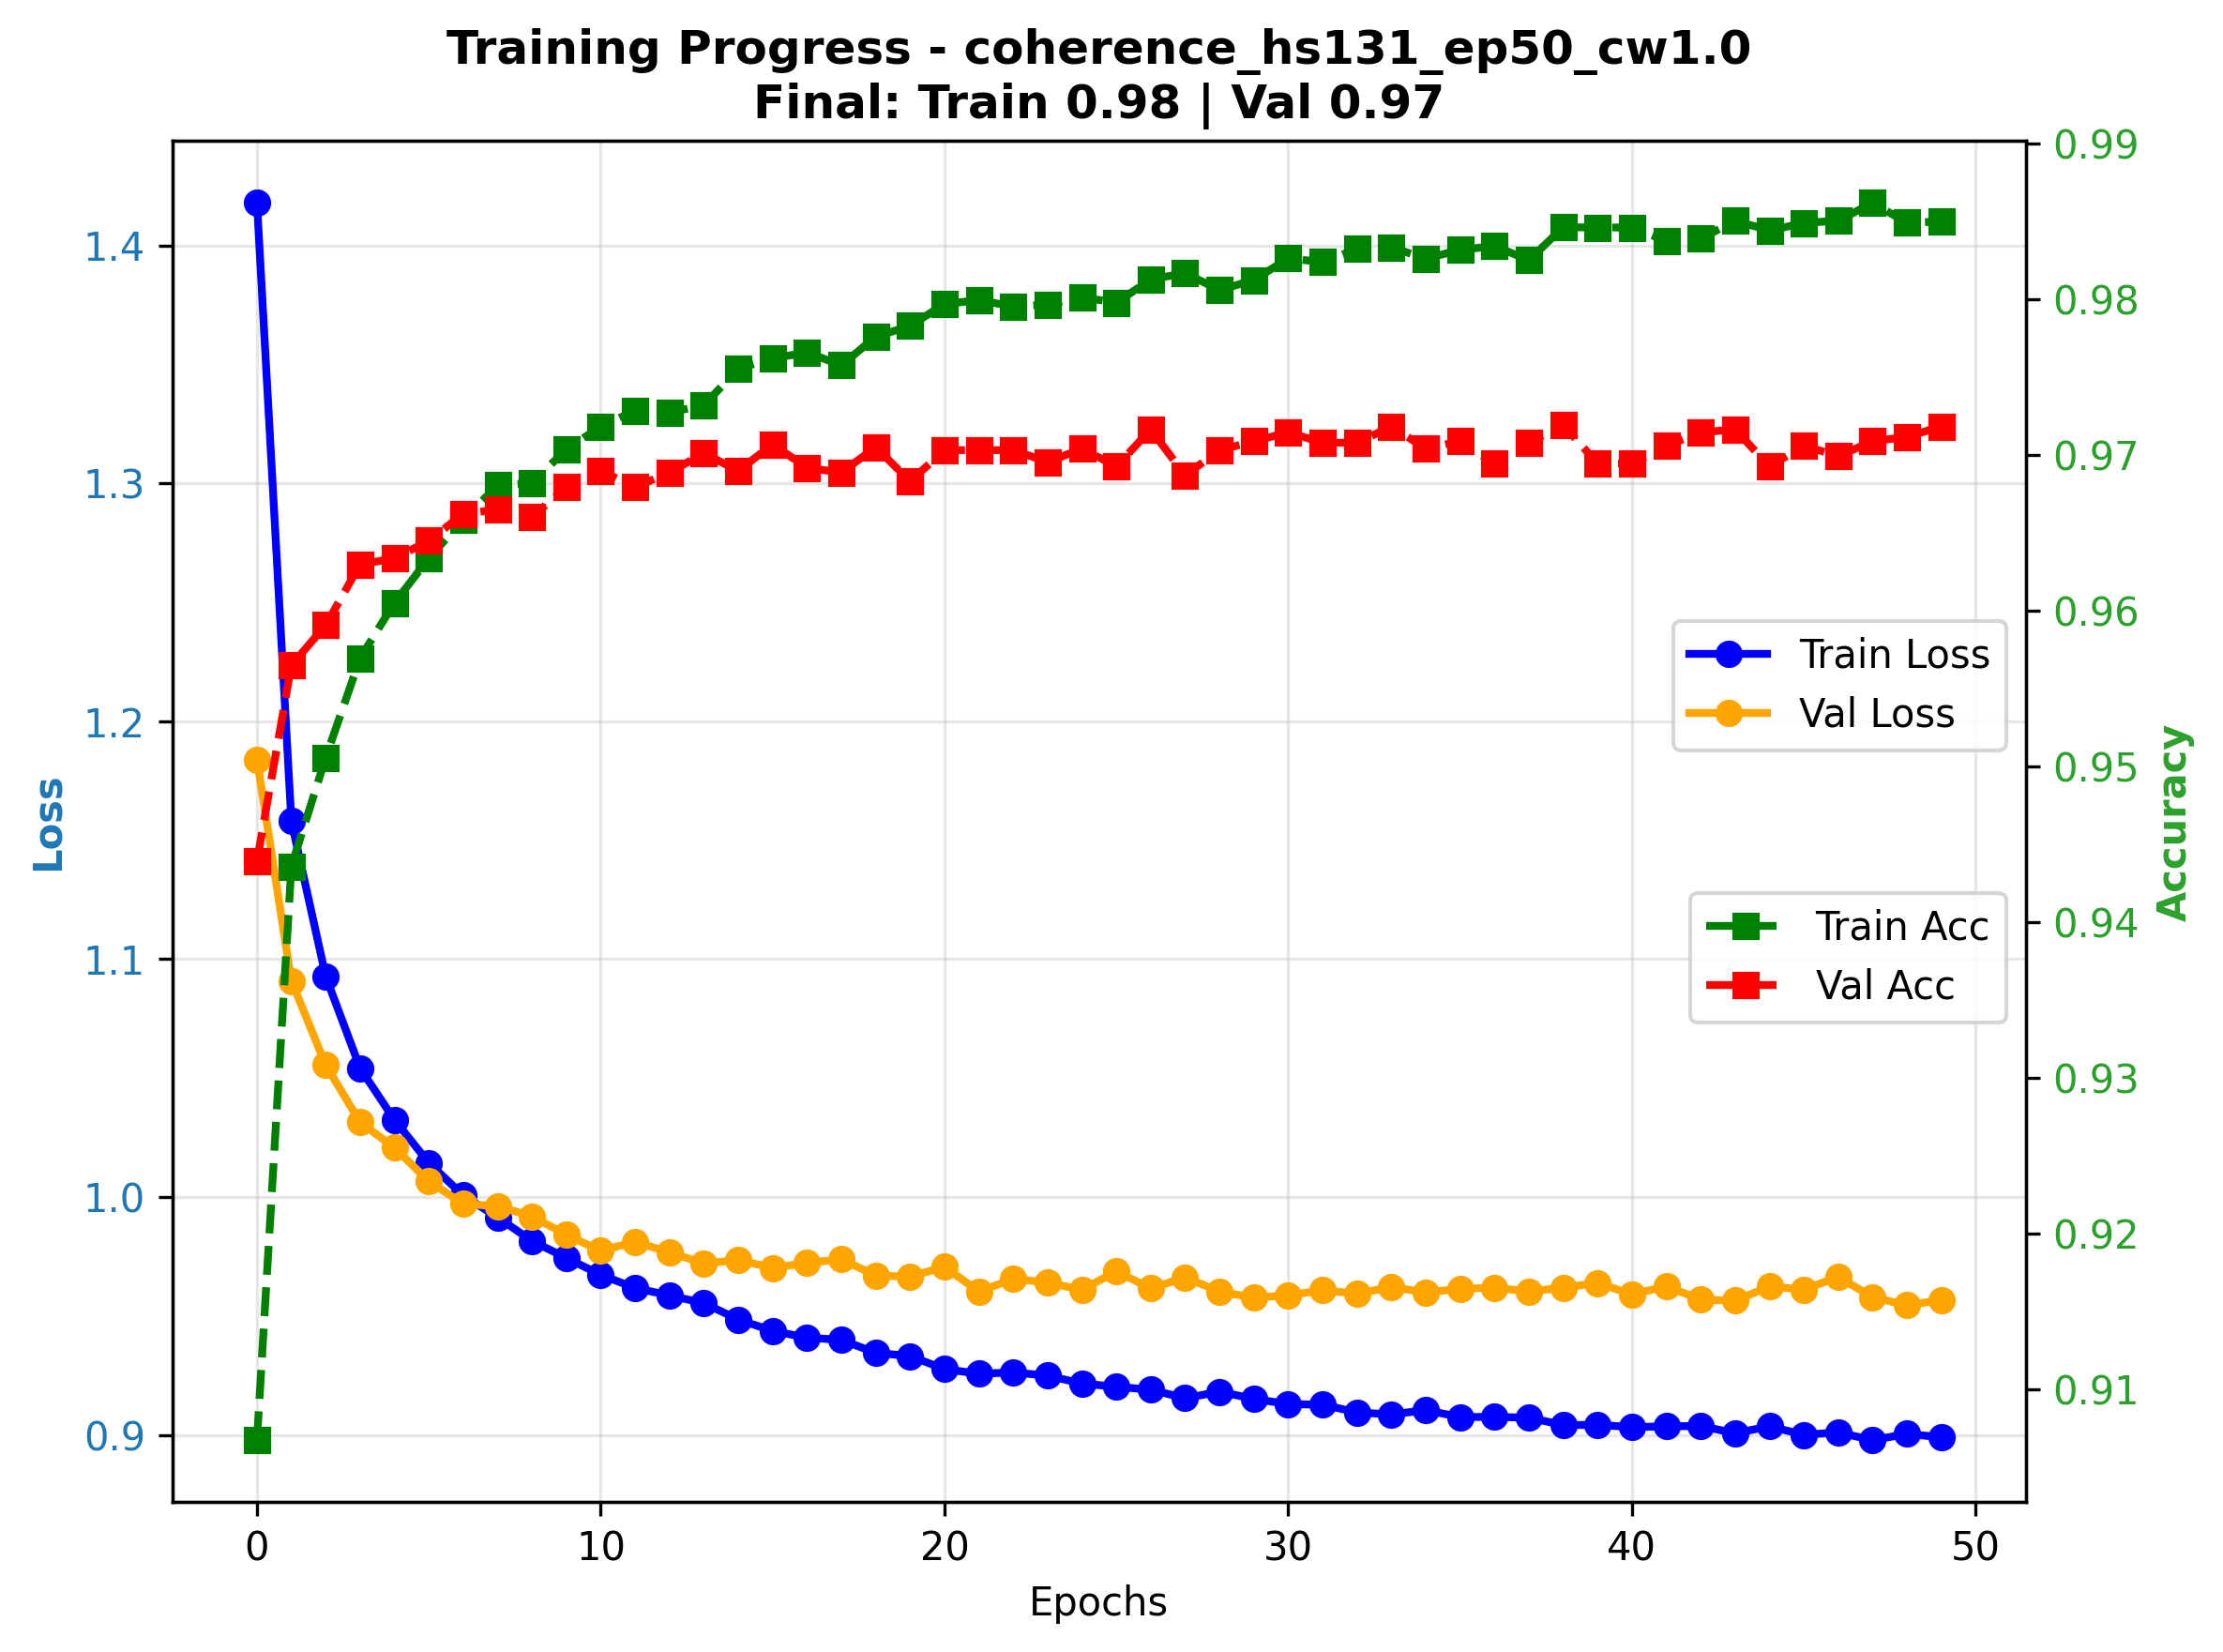
\includegraphics[width=\textwidth,height=0.48\textheight,keepaspectratio]{../plots/mlp/mnist/hs131_ep50/coherence_hs131_ep50_cw1.0_training_curves.png} \\
            \vspace{0.5em}
            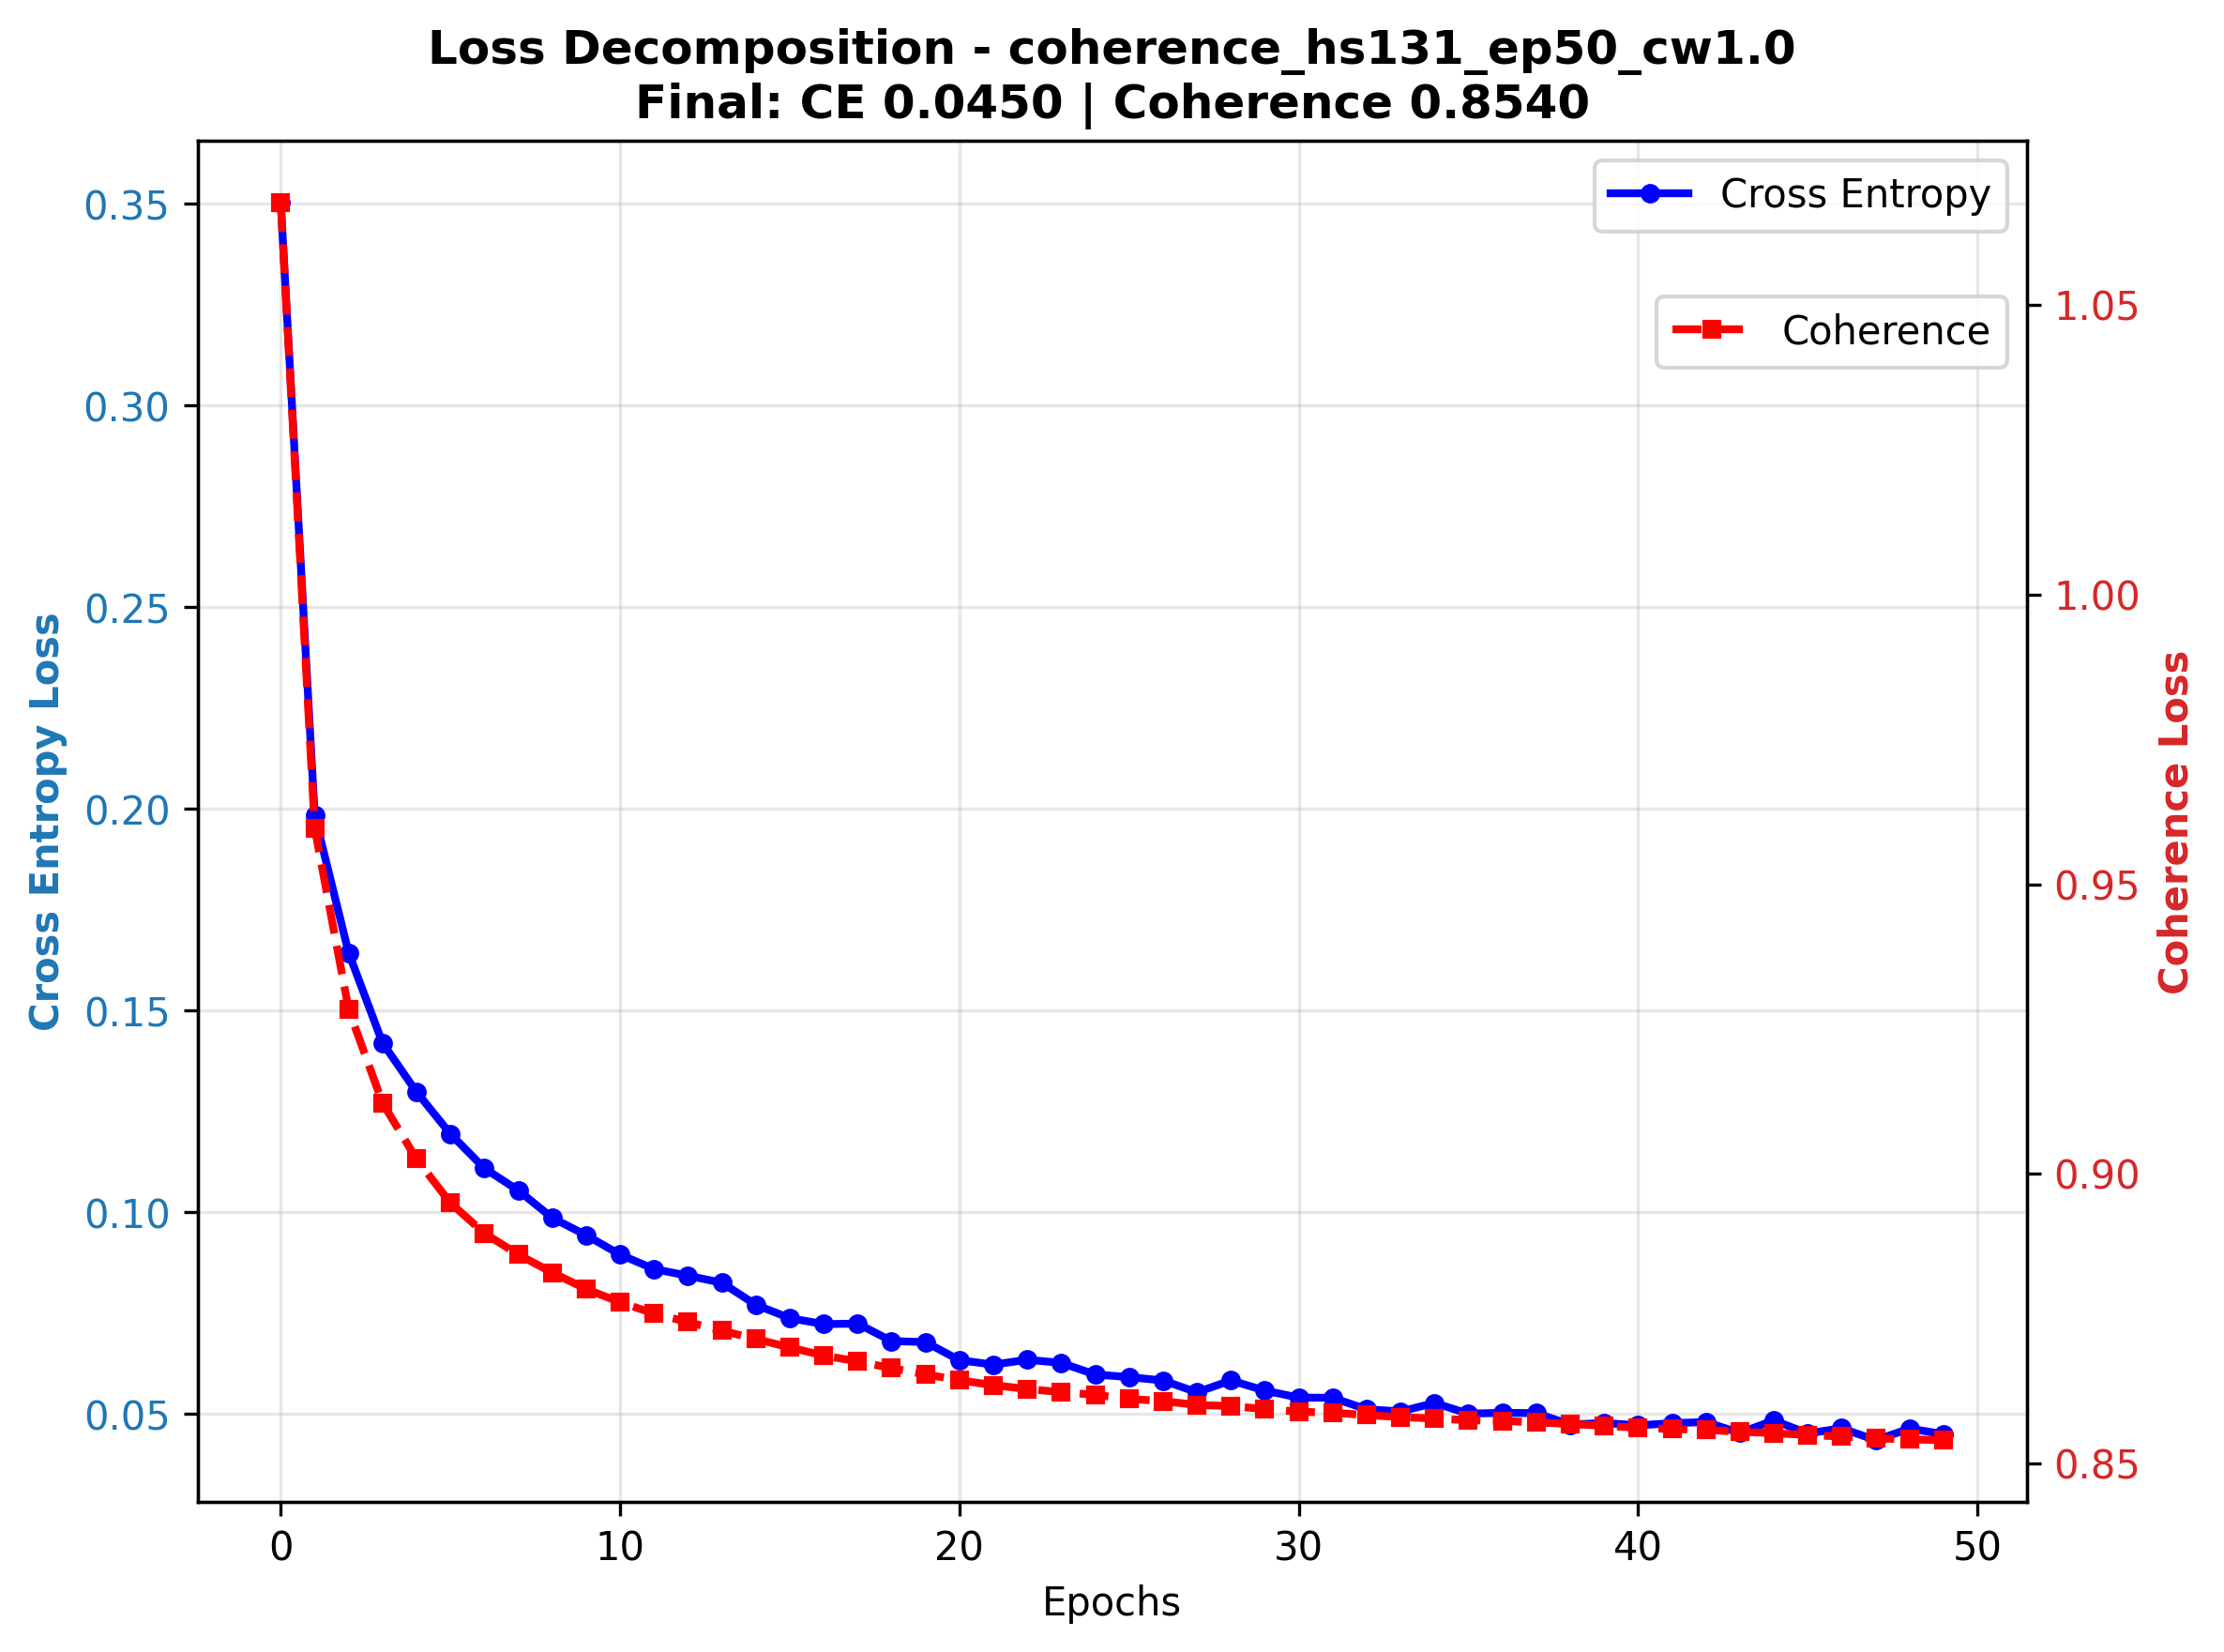
\includegraphics[width=\textwidth,height=0.48\textheight,keepaspectratio]{../plots/mlp/mnist/hs131_ep50/coherence_hs131_ep50_cw1.0_loss_decomposition.png}
        \end{minipage}
    \end{figure}

\end{frame}
%--------------------------------------------------------------------------------------
\begin{frame}{Implementation Results: MNIST}
    \begin{figure}[H]
        \centering
        % 2x1 subfigures (vertical stack, reduced height and spacing)
        \begin{minipage}[b]{\textwidth}
            \centering
            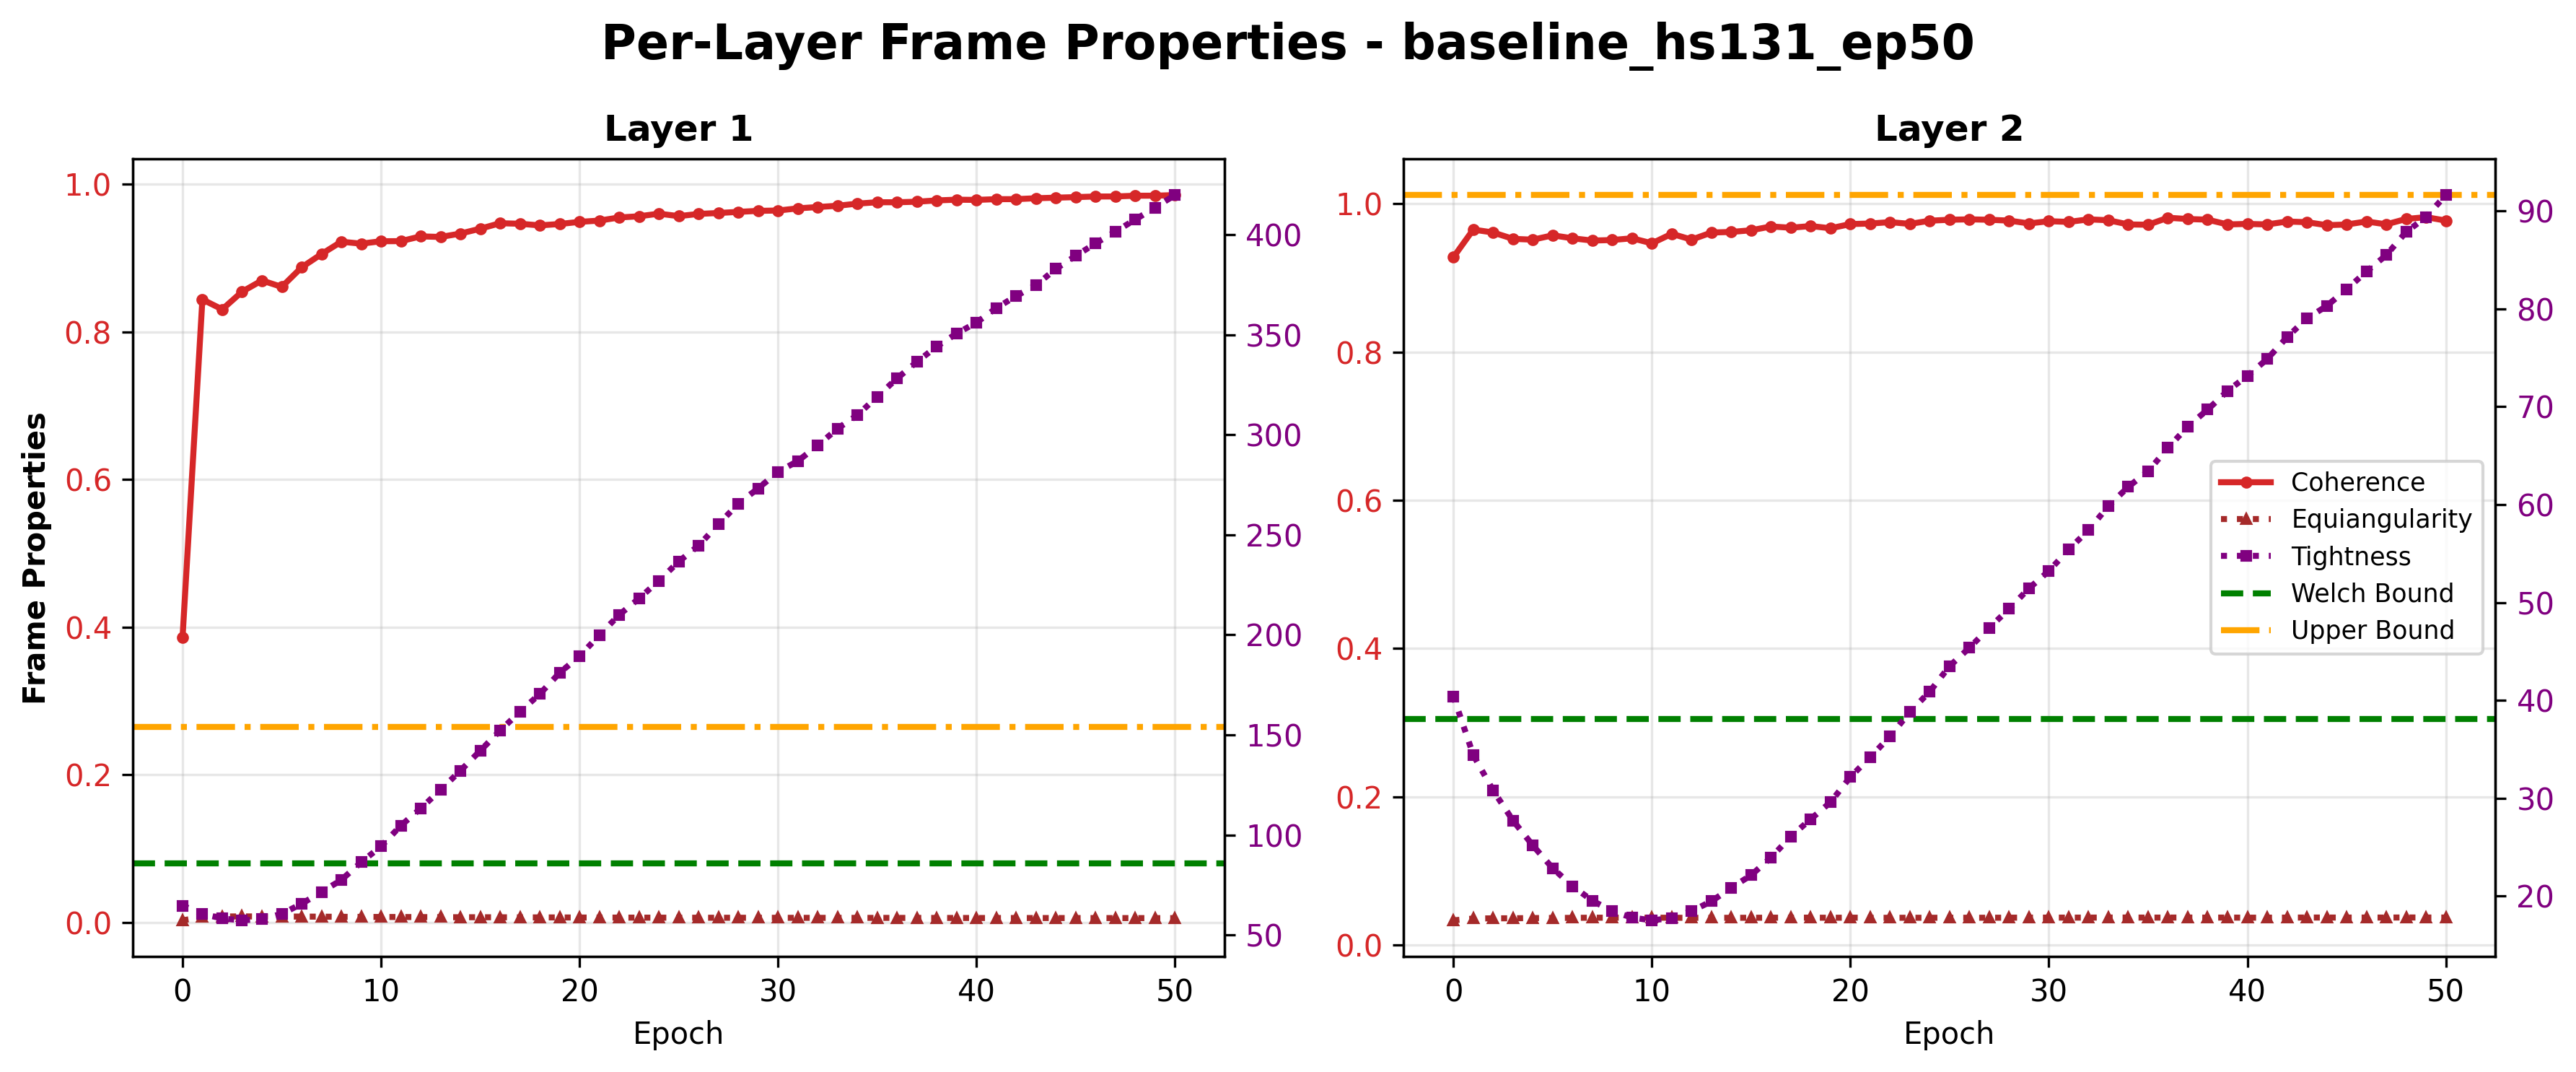
\includegraphics[width=\textwidth,height=0.45\textheight,keepaspectratio]{../plots/mlp/mnist/hs131_ep50/baseline_hs131_ep50_coherence_analysis.png}
        \end{minipage}\\[0.1em]
        \begin{minipage}[b]{\textwidth}
            \centering
            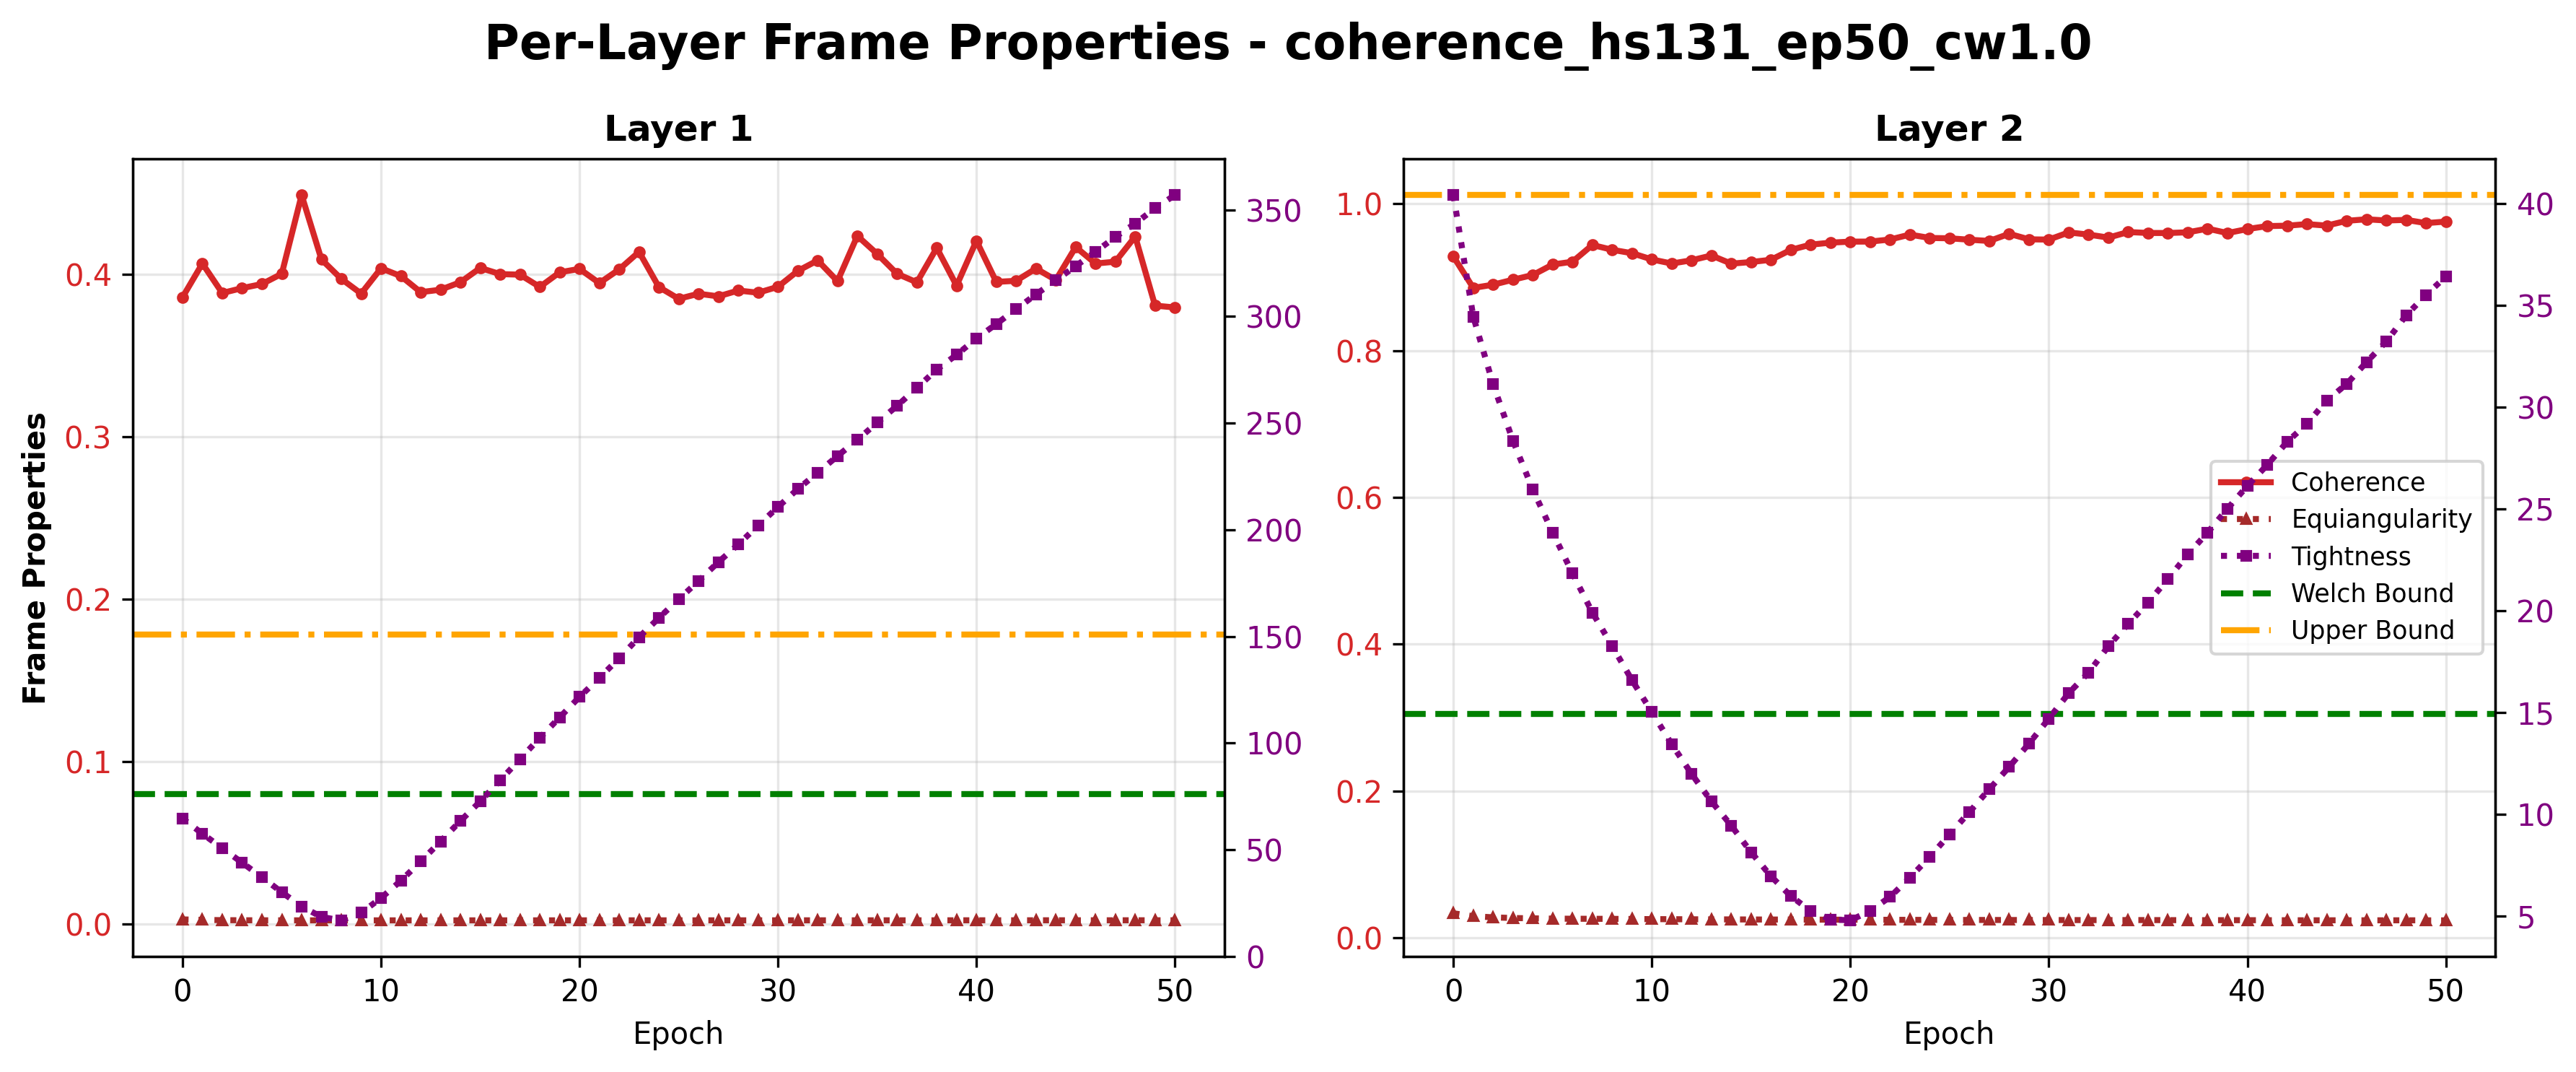
\includegraphics[width=\textwidth,height=0.45\textheight,keepaspectratio]{../plots/mlp/mnist/hs131_ep50/coherence_hs131_ep50_cw1.0_coherence_analysis.png}
        \end{minipage}
    \end{figure}
\end{frame}
%--------------------------------------------------------------------------------------
\begin{frame}{Implementation Results: MNIST}
    \begin{figure}[H]
        \centering
        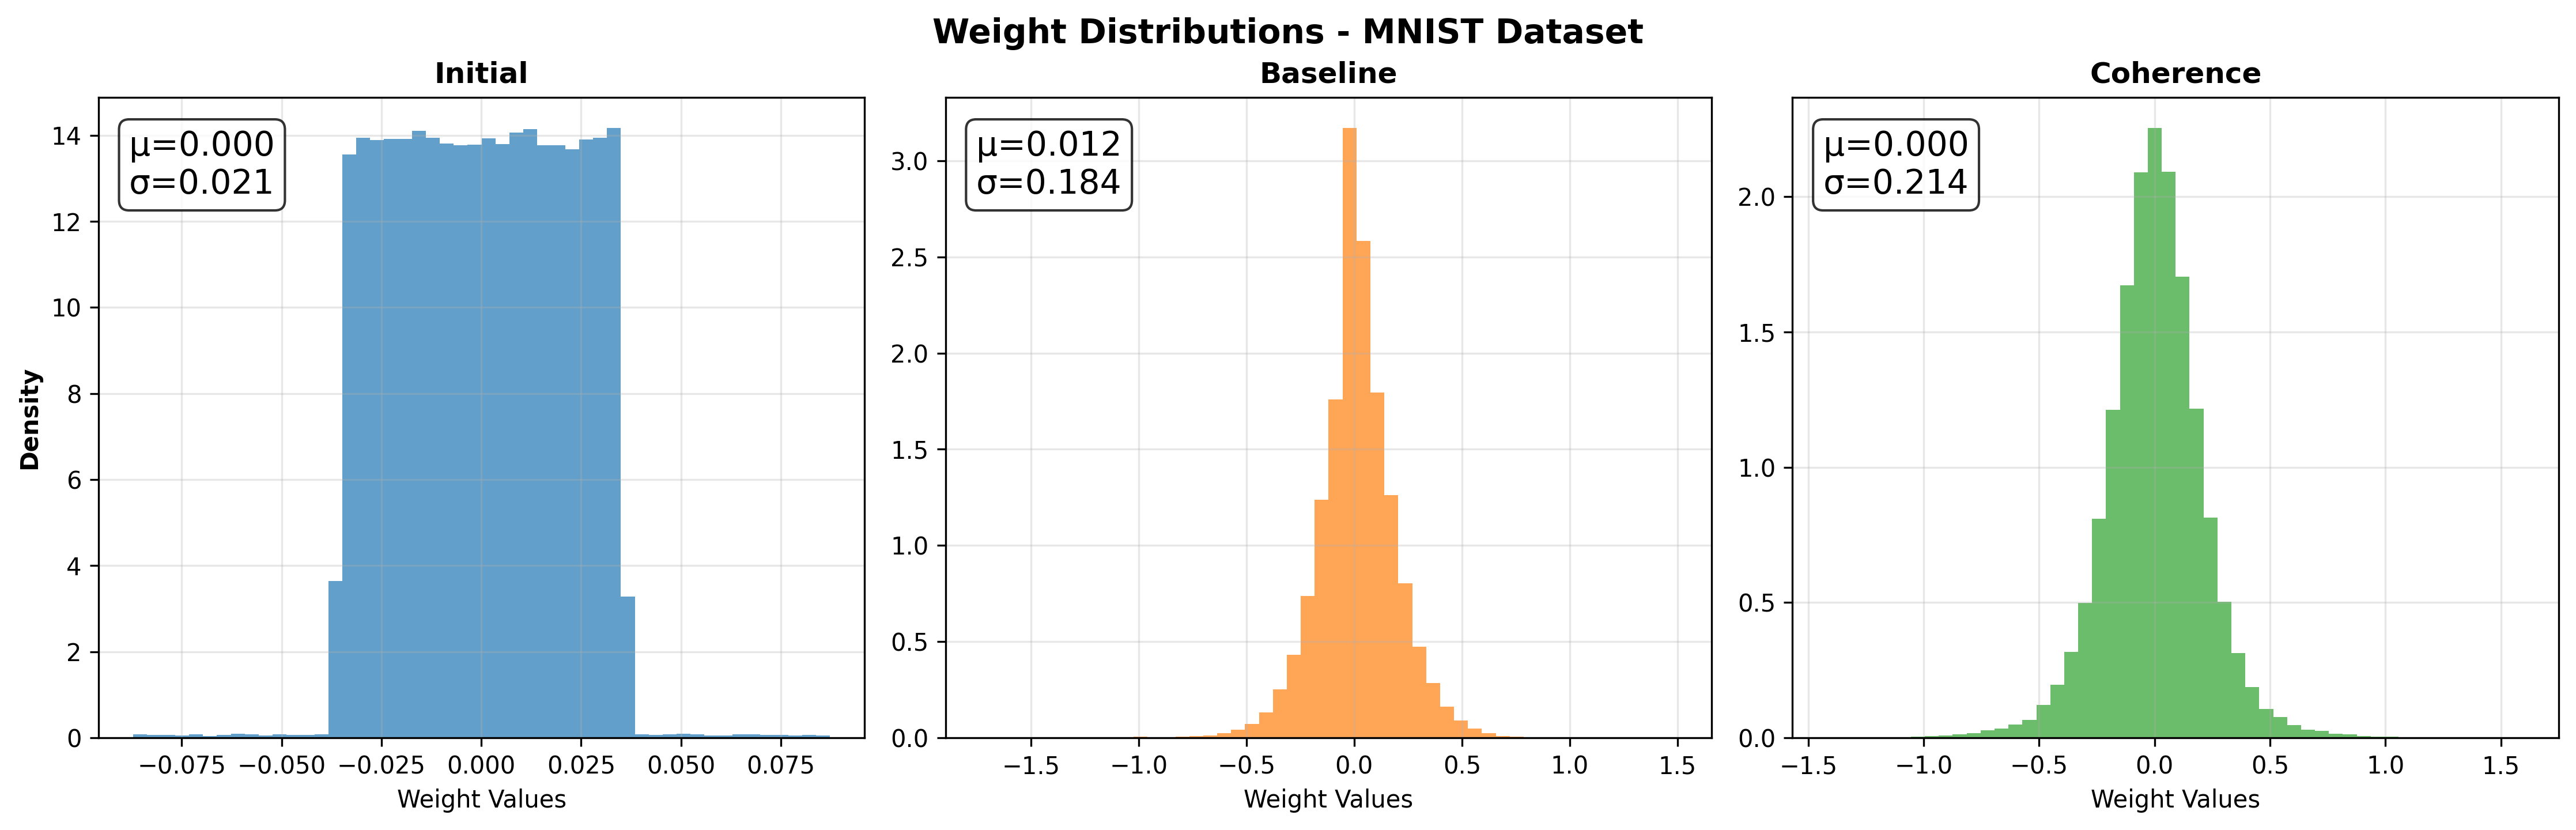
\includegraphics[width=\textwidth]{../plots/mlp/mnist/hs131_ep50/weights_distribution_cw1.0_a0.0_b0.0.png}
    \end{figure}

	\textbf{Remark:} Regularization = Coherence.
\end{frame}
%--------------------------------------------------------------------------------------
\begin{frame}[c]

	\centering

	{\Huge \textbf{Thank you for your}}

	\vspace{0.5cm}

	{\Huge
		\begin{equation*}
			{\color{blue}\boldsymbol{\softmax\left(\frac{QK^\top}{\sqrt{d_k}} \odot M \right)V}}
		\end{equation*}
	}

	\vspace{0.5cm}

\end{frame}
%--------------------------------------------------------------------------------------
% References Frame
\begin{frame}[allowframebreaks]{References}
	\tiny
	\printbibliography % Use biblatex's \printbibliography for numbered references
\end{frame}
%--------------------------------------------------------------------------------------
\section{Annex}
\begin{frame}[c]

    \centering
    \Huge \textbf{Annex}

\end{frame}
%--------------------------------------------------------------------------------------
\subsection{Low Coherence MLPs: Fashion MNIST}
\begin{frame}{Implementation Results: Fashion MNIST}

    % 2-column figure: baseline (left), coherence model (right, stacked)
    
    \begin{figure}[H]
        \centering
        \begin{minipage}[b]{0.48\textwidth}
            \centering
            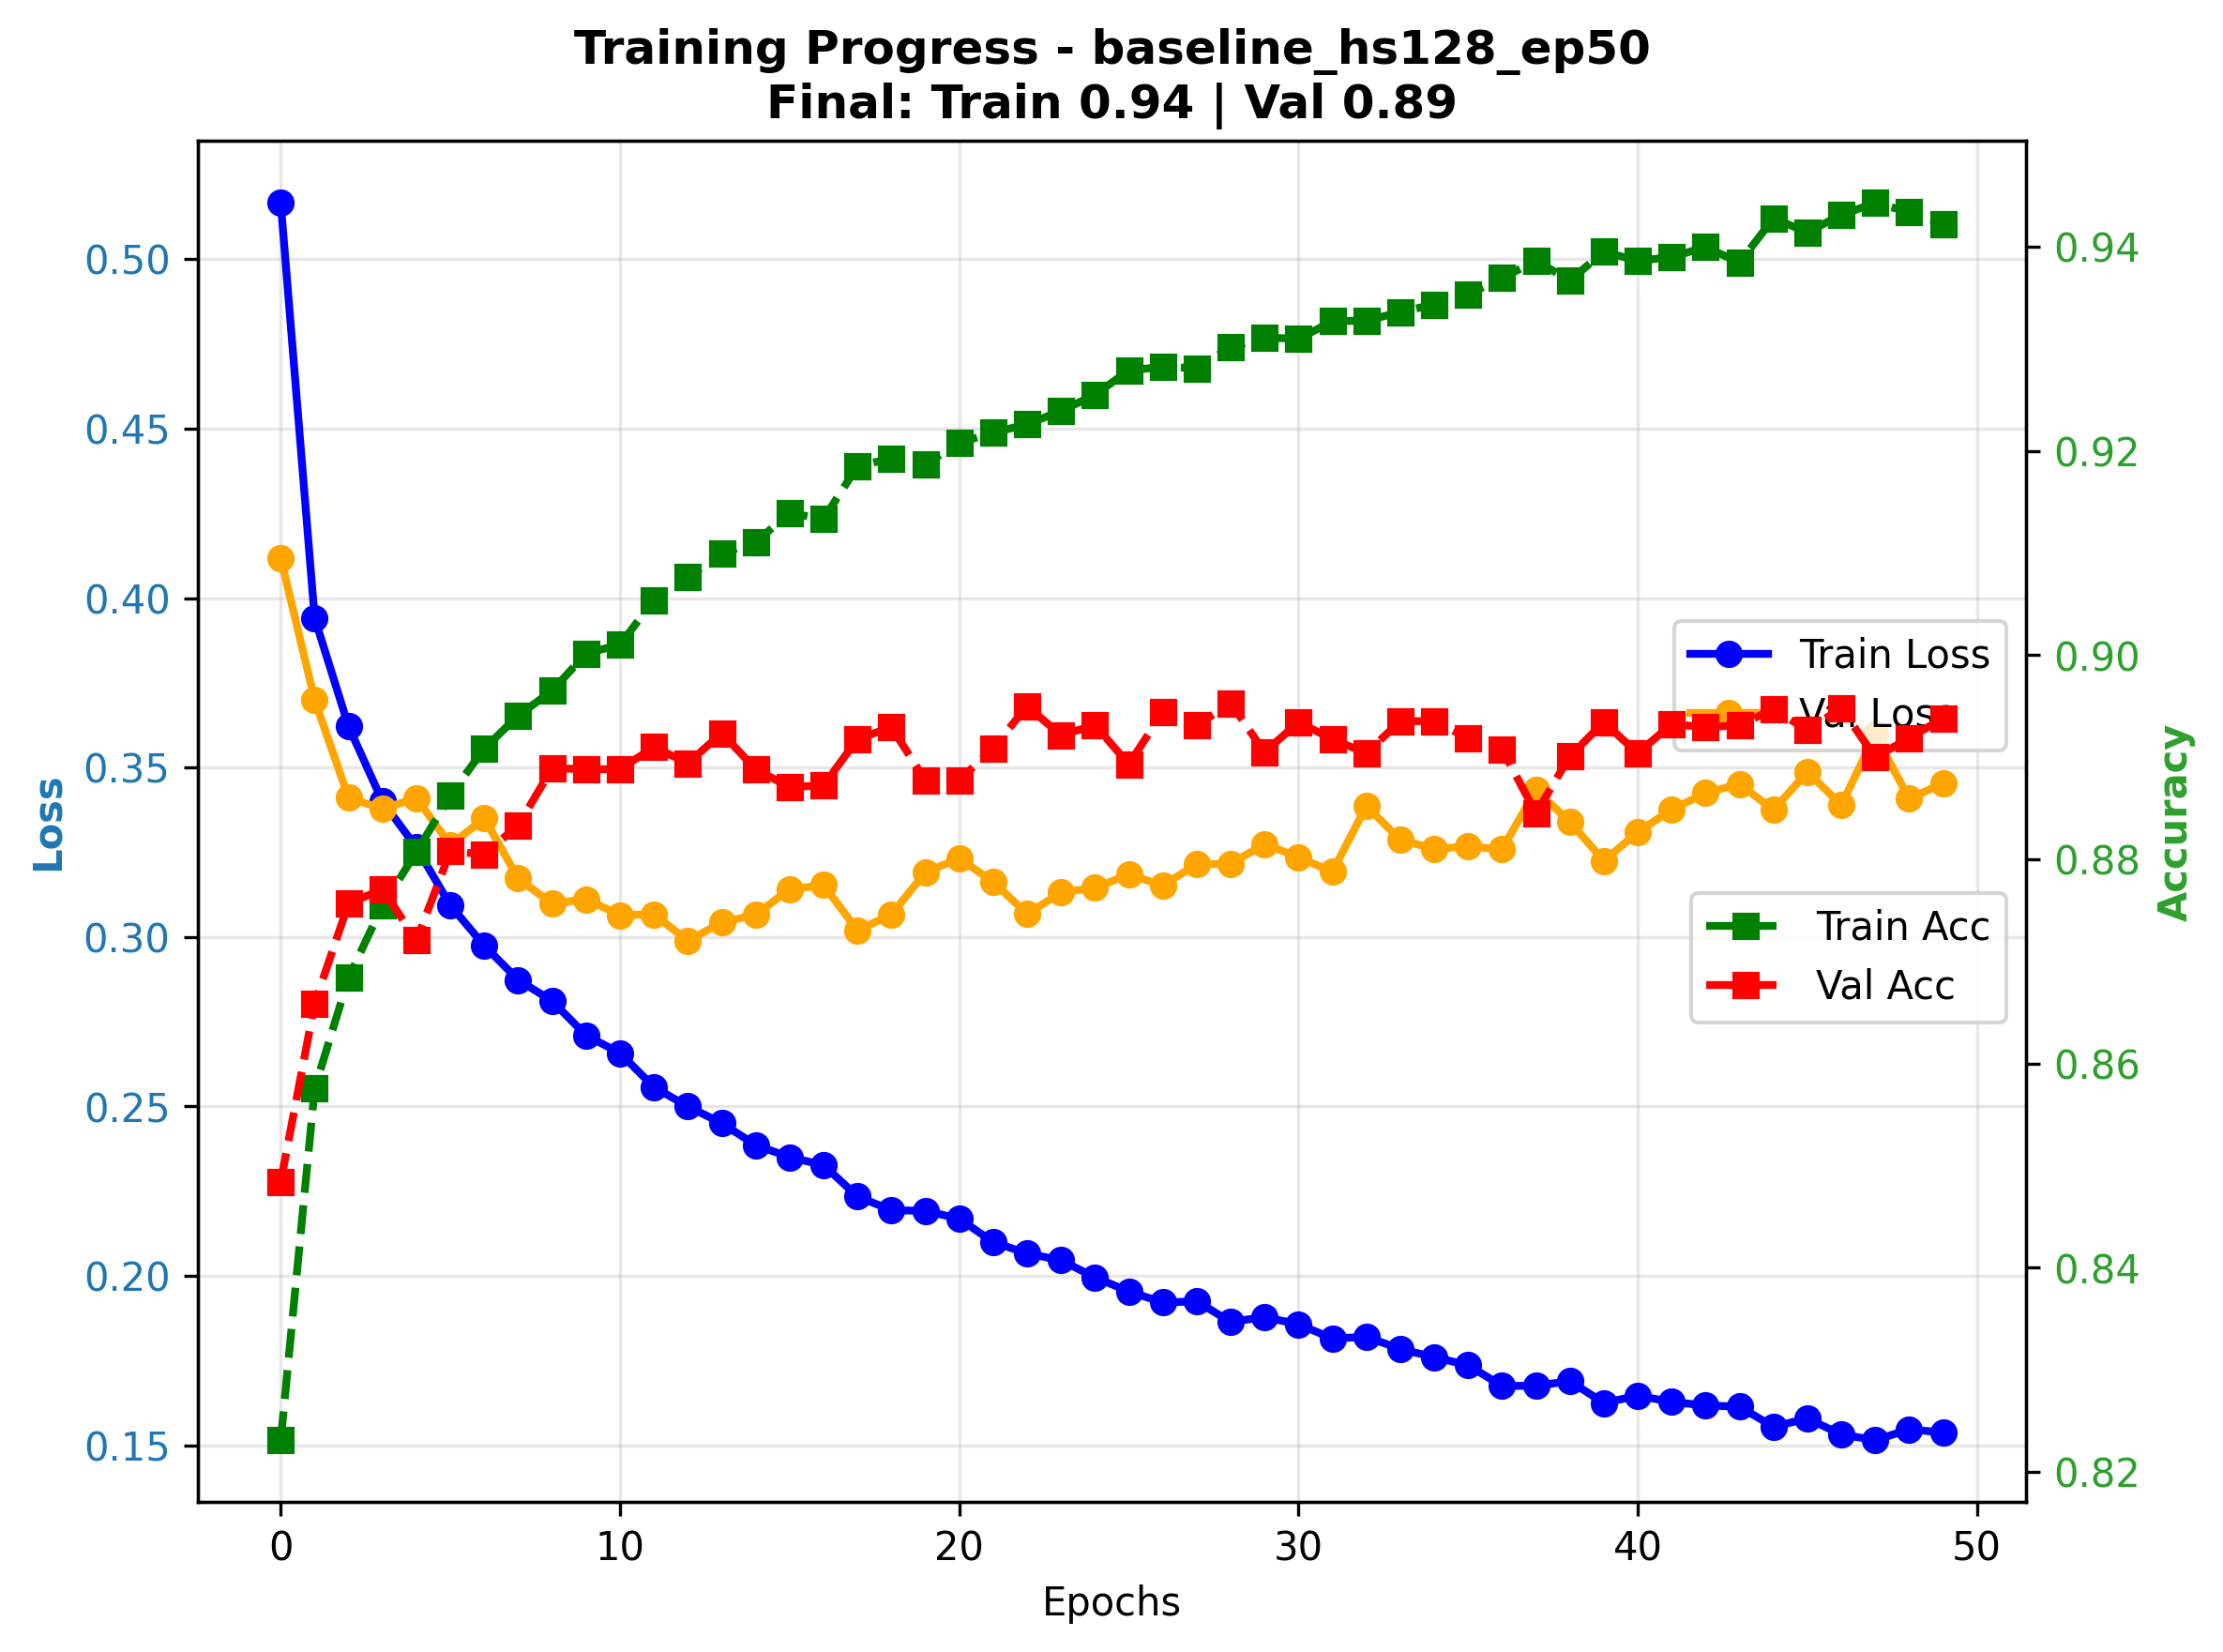
\includegraphics[width=\textwidth]{../plots/mlp/fashion_mnist/hs128_ep50/baseline_hs128_ep50_training_curves.png}
            
            \vspace{0.1\textheight}
            {\scriptsize
            \begin{tabular}{lcc}
                \toprule
                & \textbf{Baseline} & \textbf{Coherence} \\
                \midrule
                Final Test Loss & 0.37 & 0.61 \\
                Final Test Accuracy & 0.89 & \textbf{\textcolor{red}{0.89}} \\
                Best Epoch & 28 & \textbf{\textcolor{red}{41}} \\
                Best Val Accuracy & 0.90 & 0.90 \\
                \bottomrule
            \end{tabular}
            }
			\vspace{0.15\textheight}
        \end{minipage}%
        \hfill
        \begin{minipage}[b]{0.48\textwidth}
            \centering
            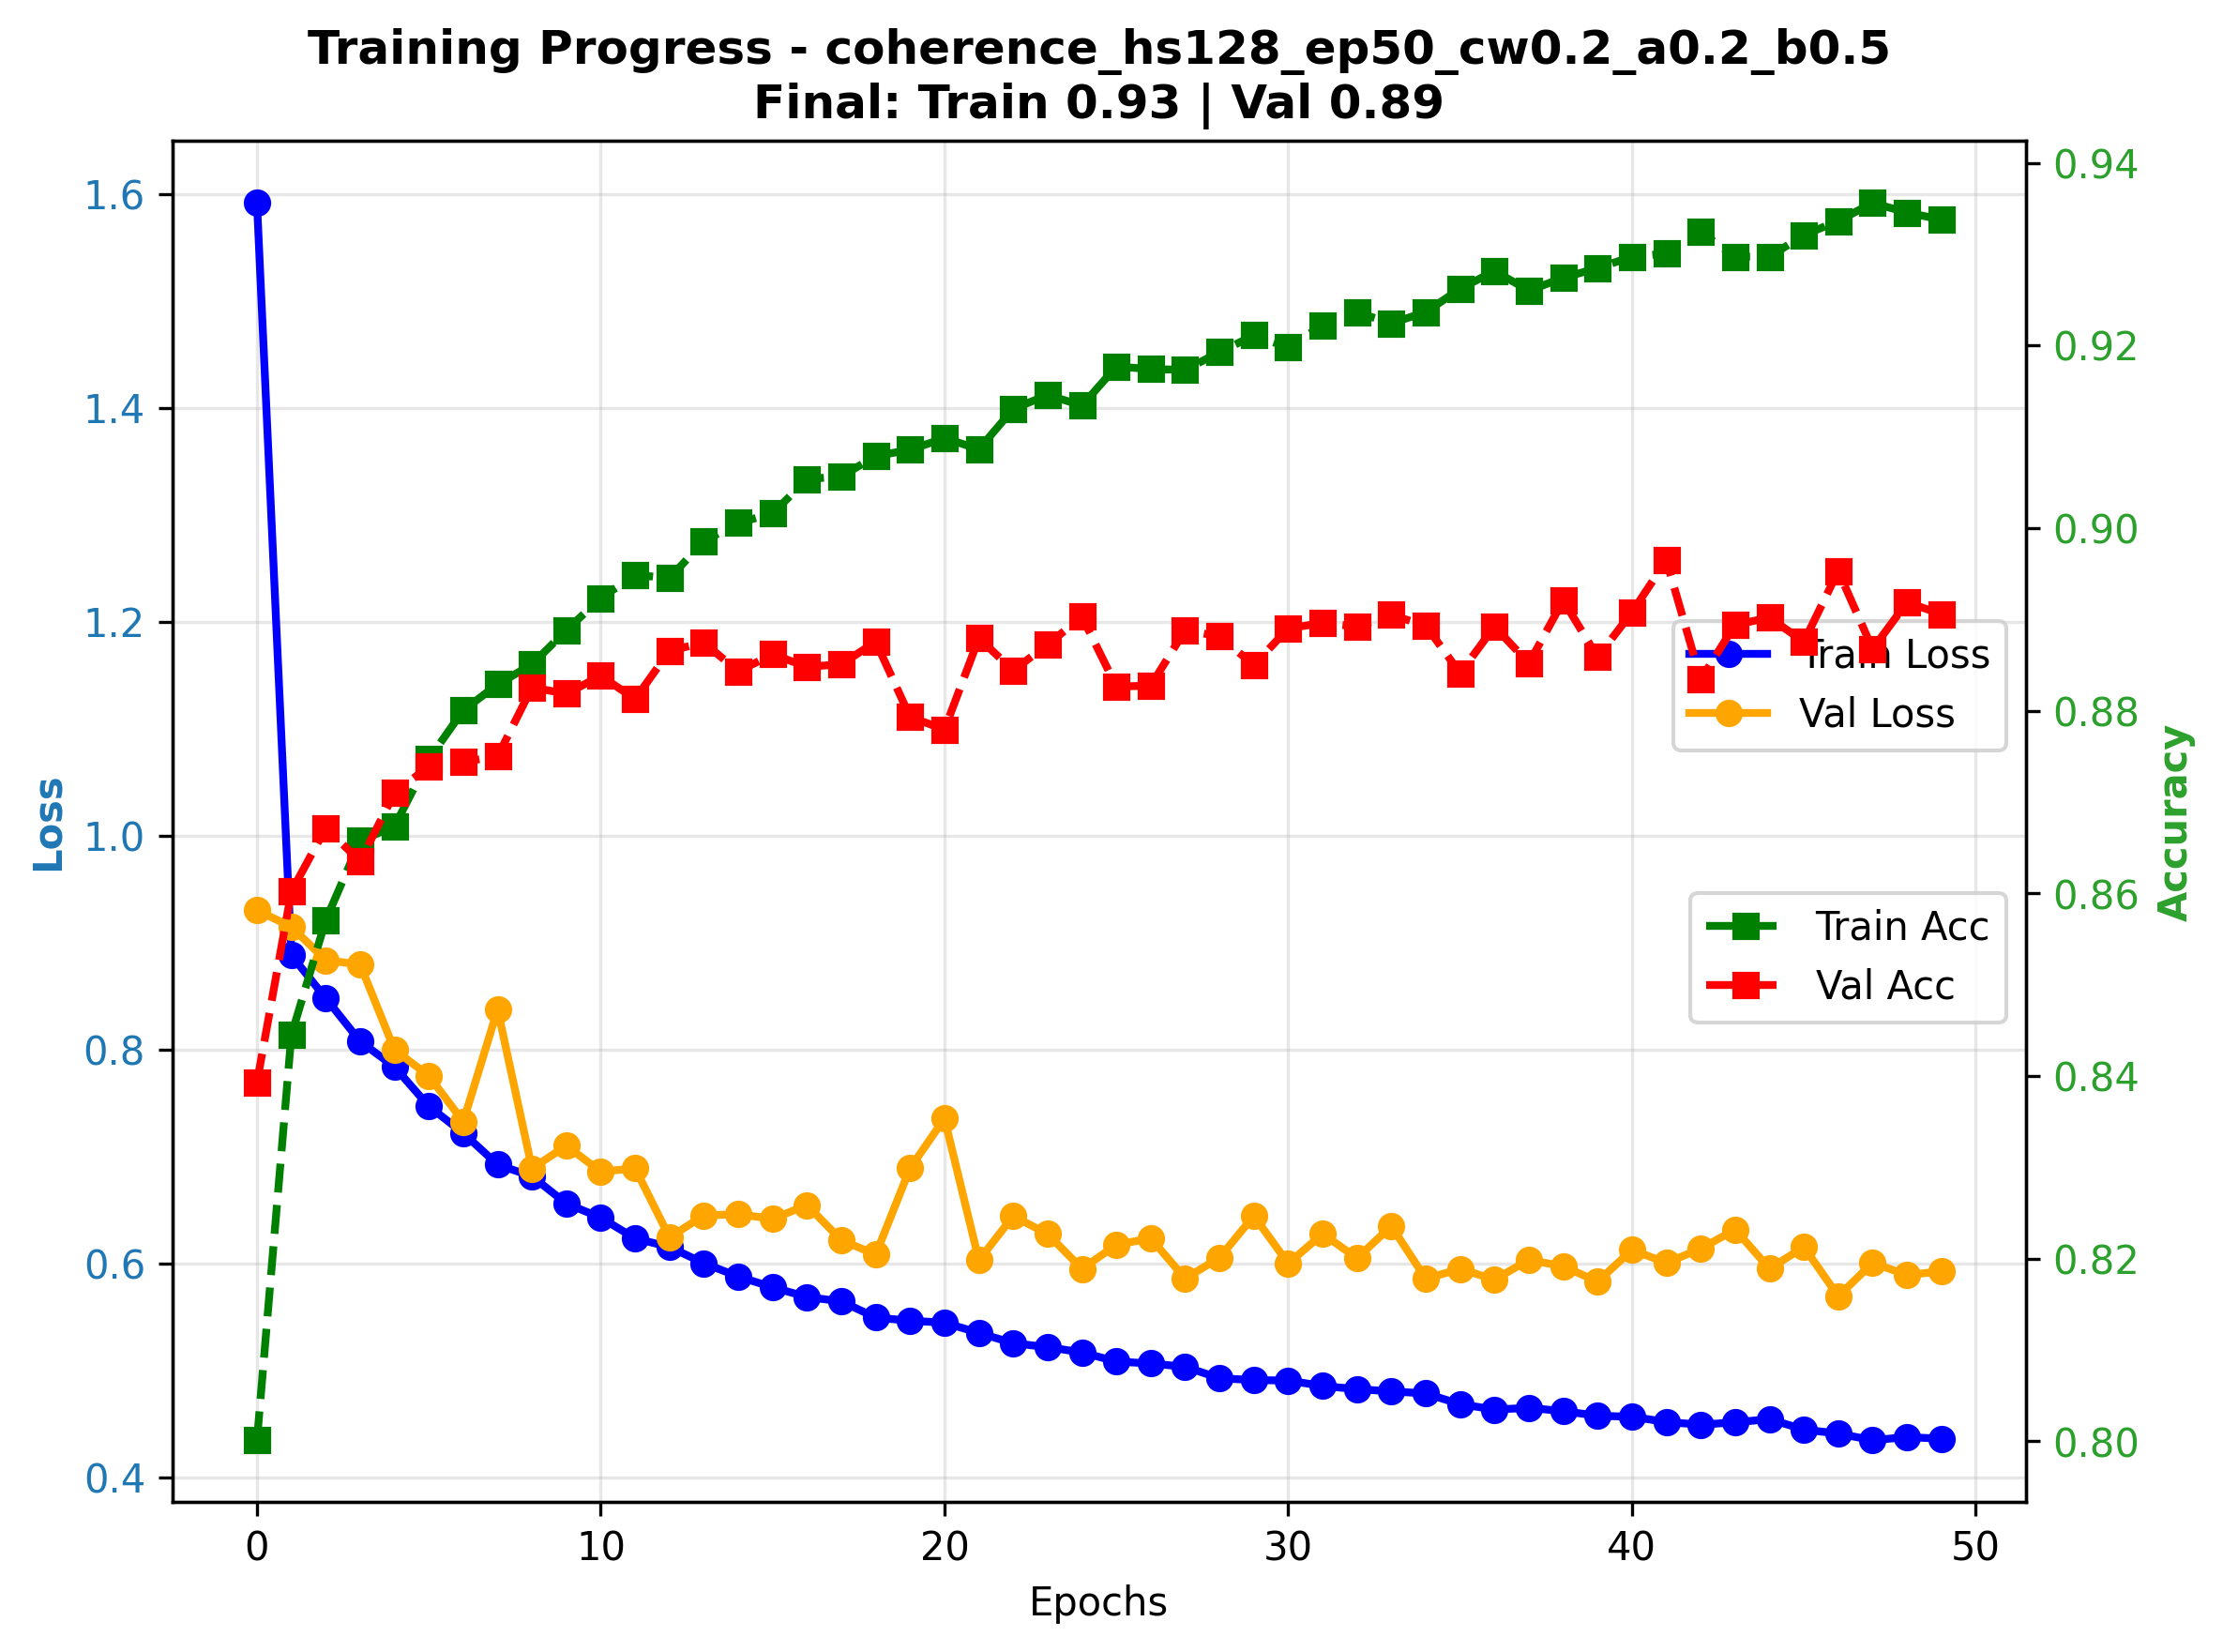
\includegraphics[width=\textwidth,height=0.48\textheight,keepaspectratio]{../plots/mlp/fashion_mnist/hs128_ep50/coherence_hs128_ep50_cw0.2_a0.2_b0.5_training_curves.png} \\
            \vspace{0.5em}
            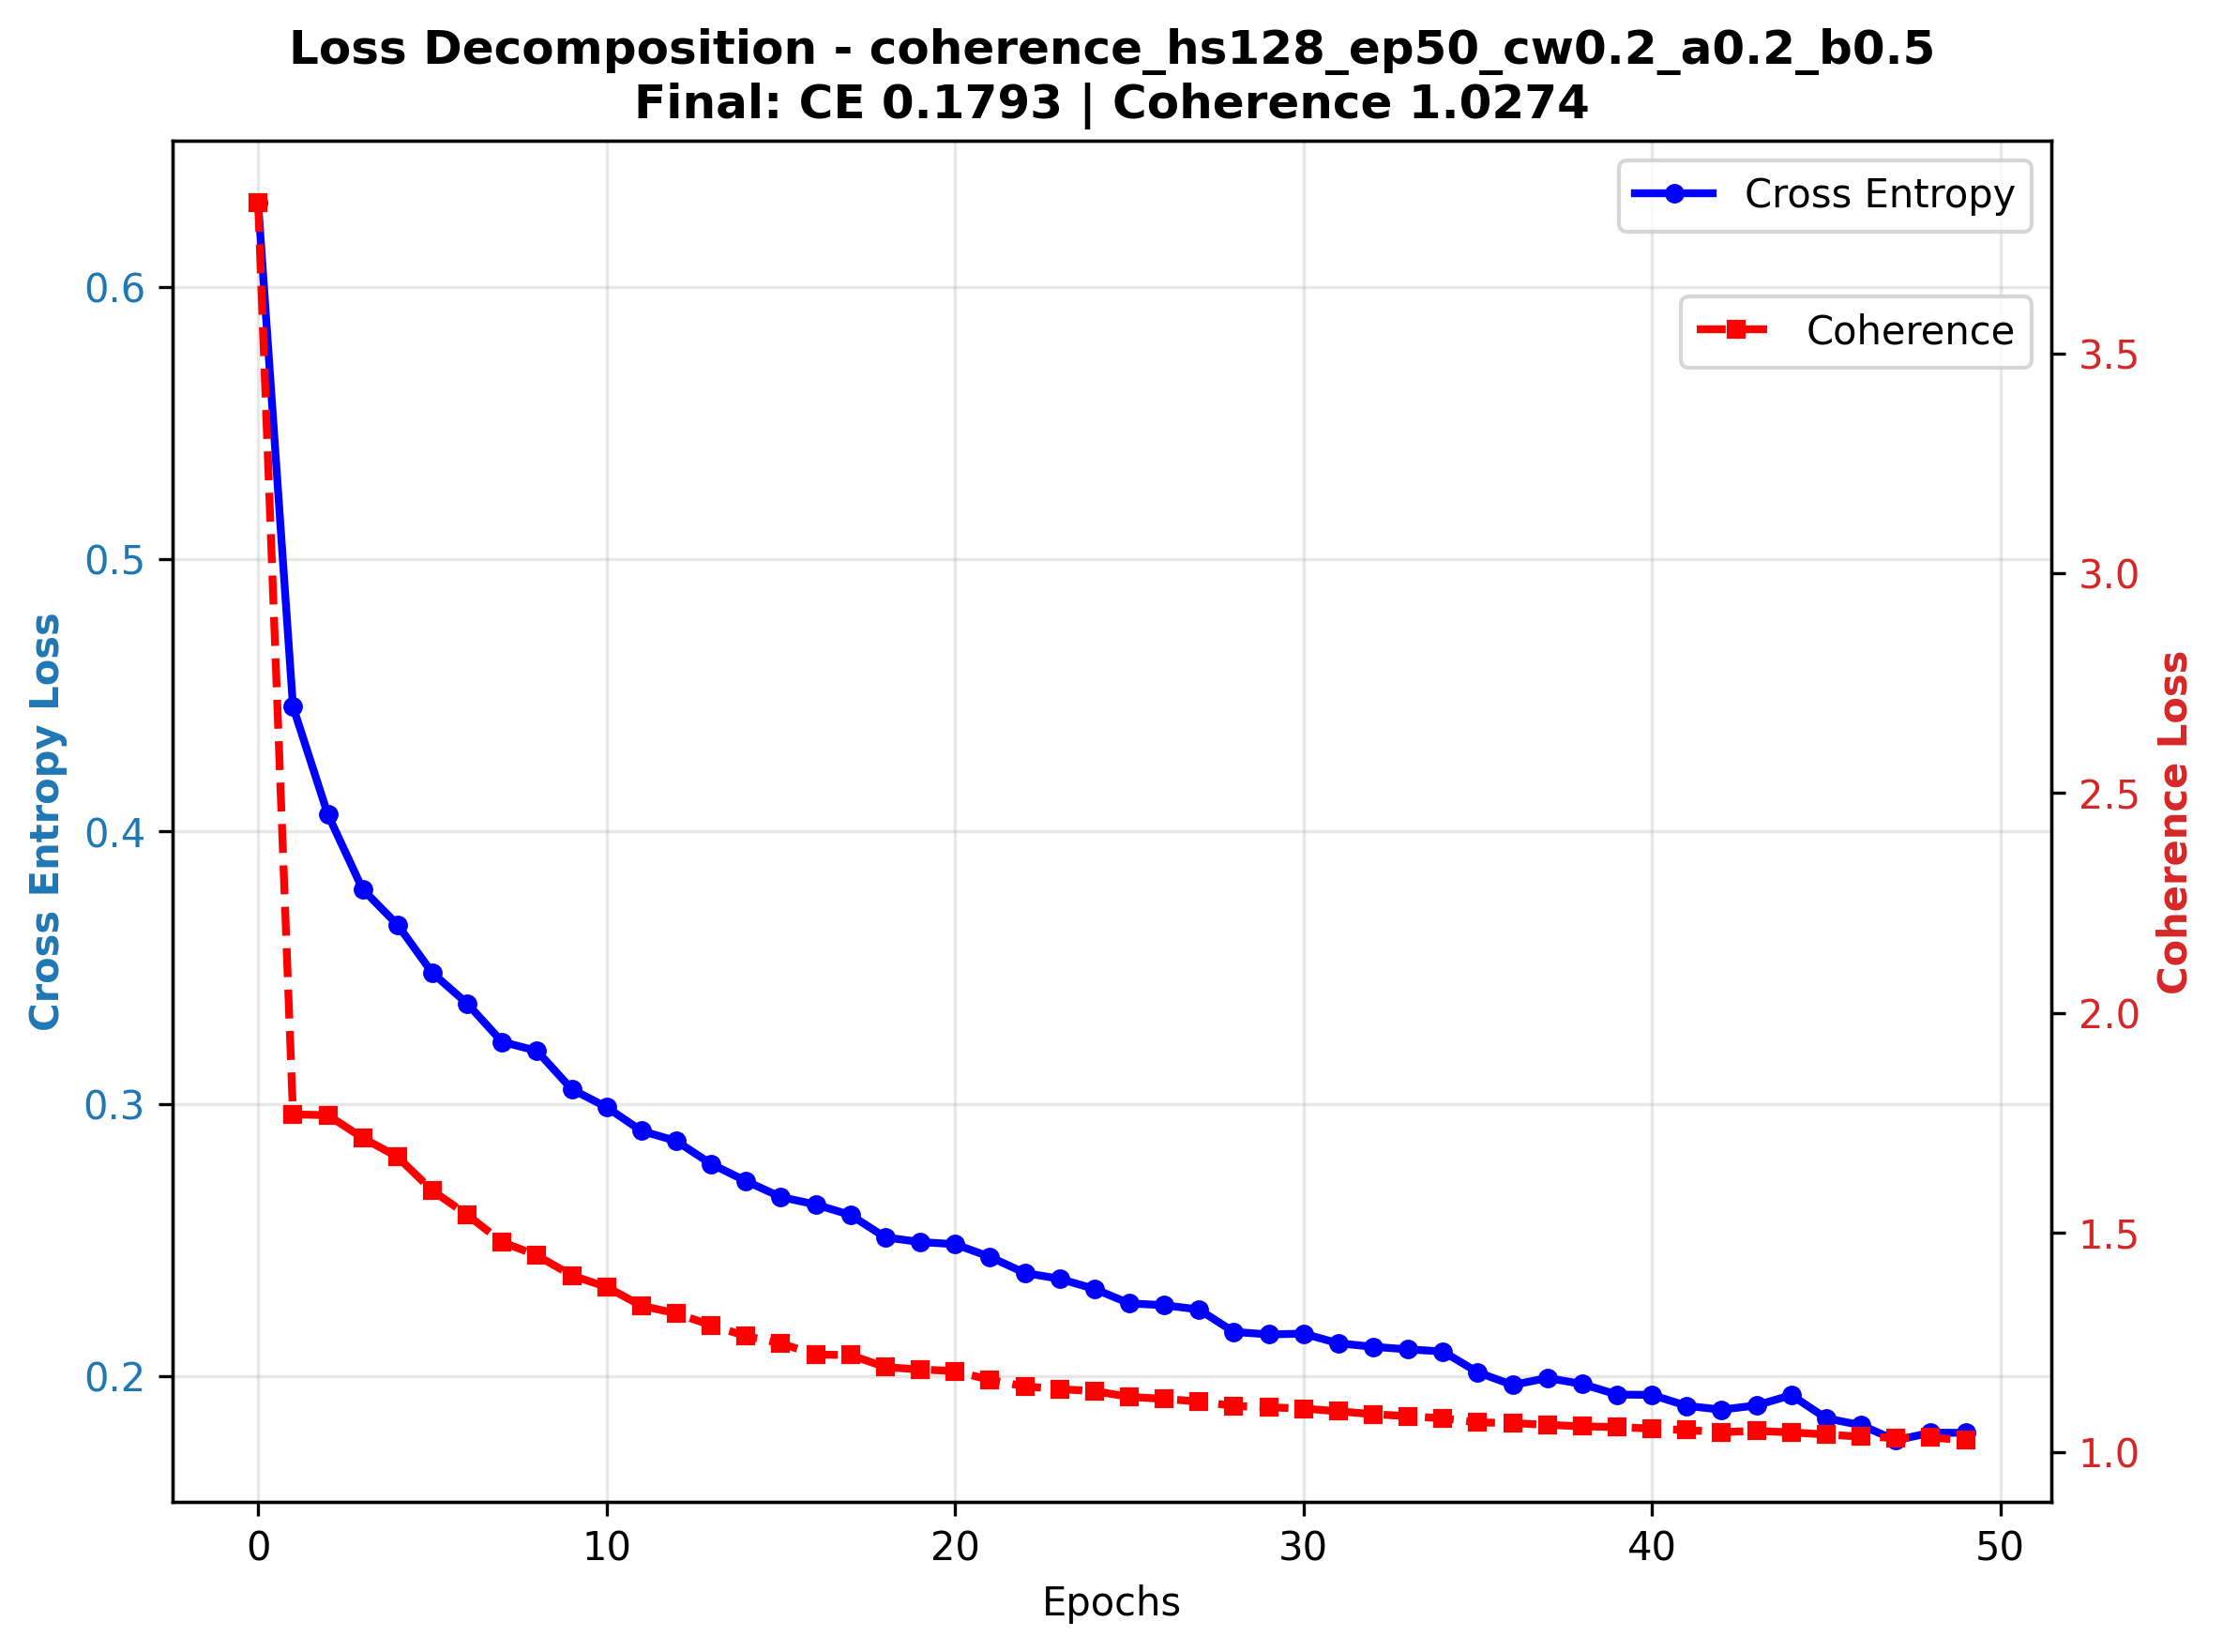
\includegraphics[width=\textwidth,height=0.48\textheight,keepaspectratio]{../plots/mlp/fashion_mnist/hs128_ep50/coherence_hs128_ep50_cw0.2_a0.2_b0.5_loss_decomposition.png}
        \end{minipage}
    \end{figure}

\end{frame}
%--------------------------------------------------------------------------------------
\begin{frame}{Implementation Results: Fashion MNIST}
    \begin{figure}[H]
        \centering
        % 2x1 subfigures (vertical stack, reduced height and spacing)
        \begin{minipage}[b]{\textwidth}
            \centering
            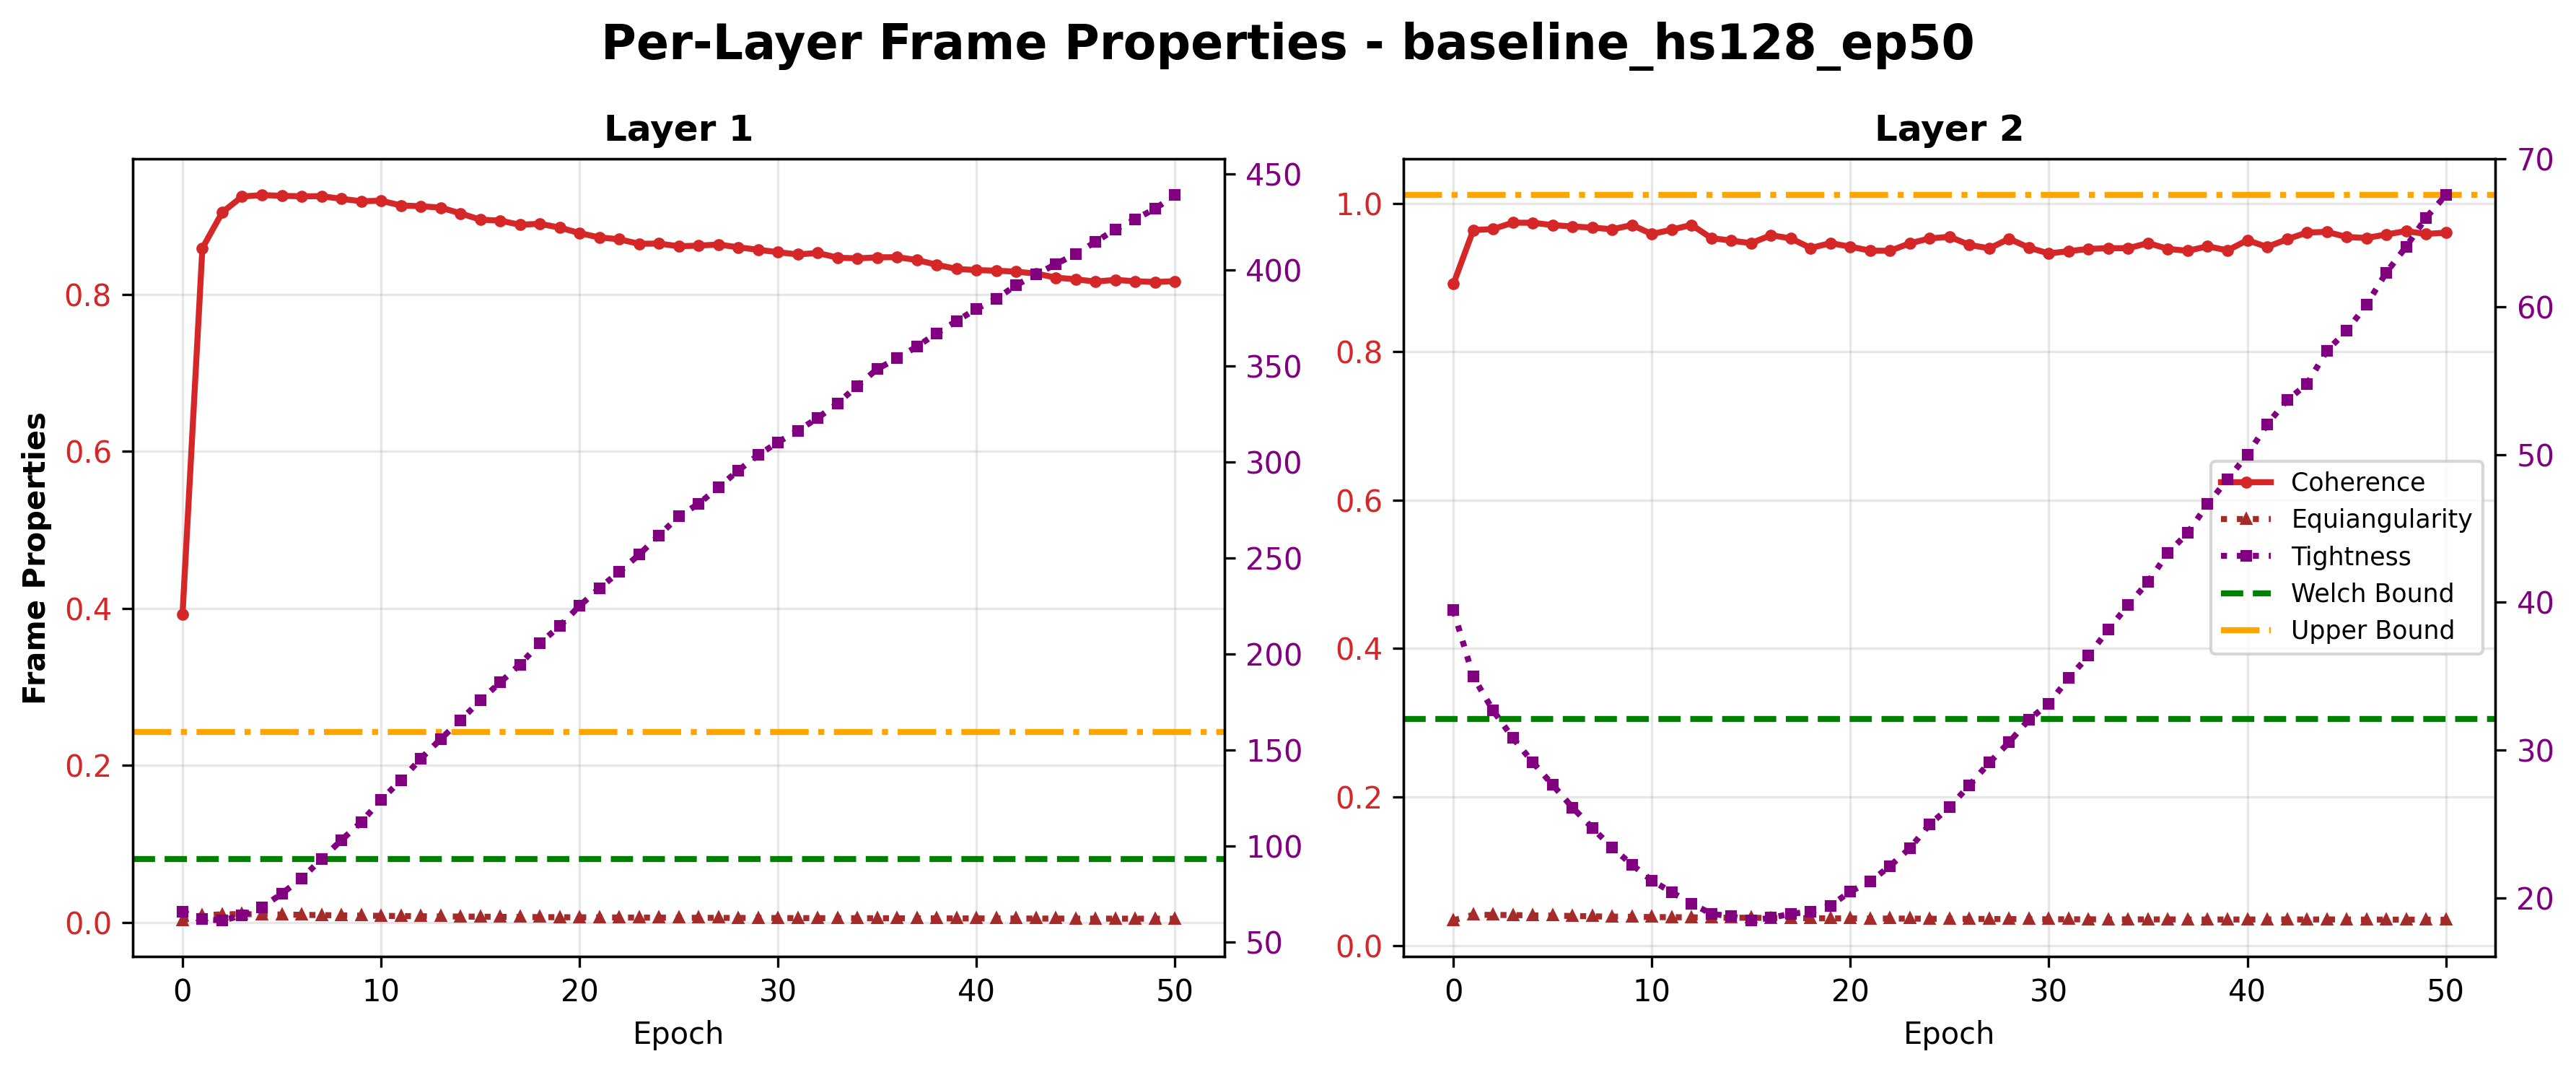
\includegraphics[width=\textwidth,height=0.45\textheight,keepaspectratio]{../plots/mlp/fashion_mnist/hs128_ep50/baseline_hs128_ep50_coherence_analysis.png}
        \end{minipage}\\[0.1em]
        \begin{minipage}[b]{\textwidth}
            \centering
            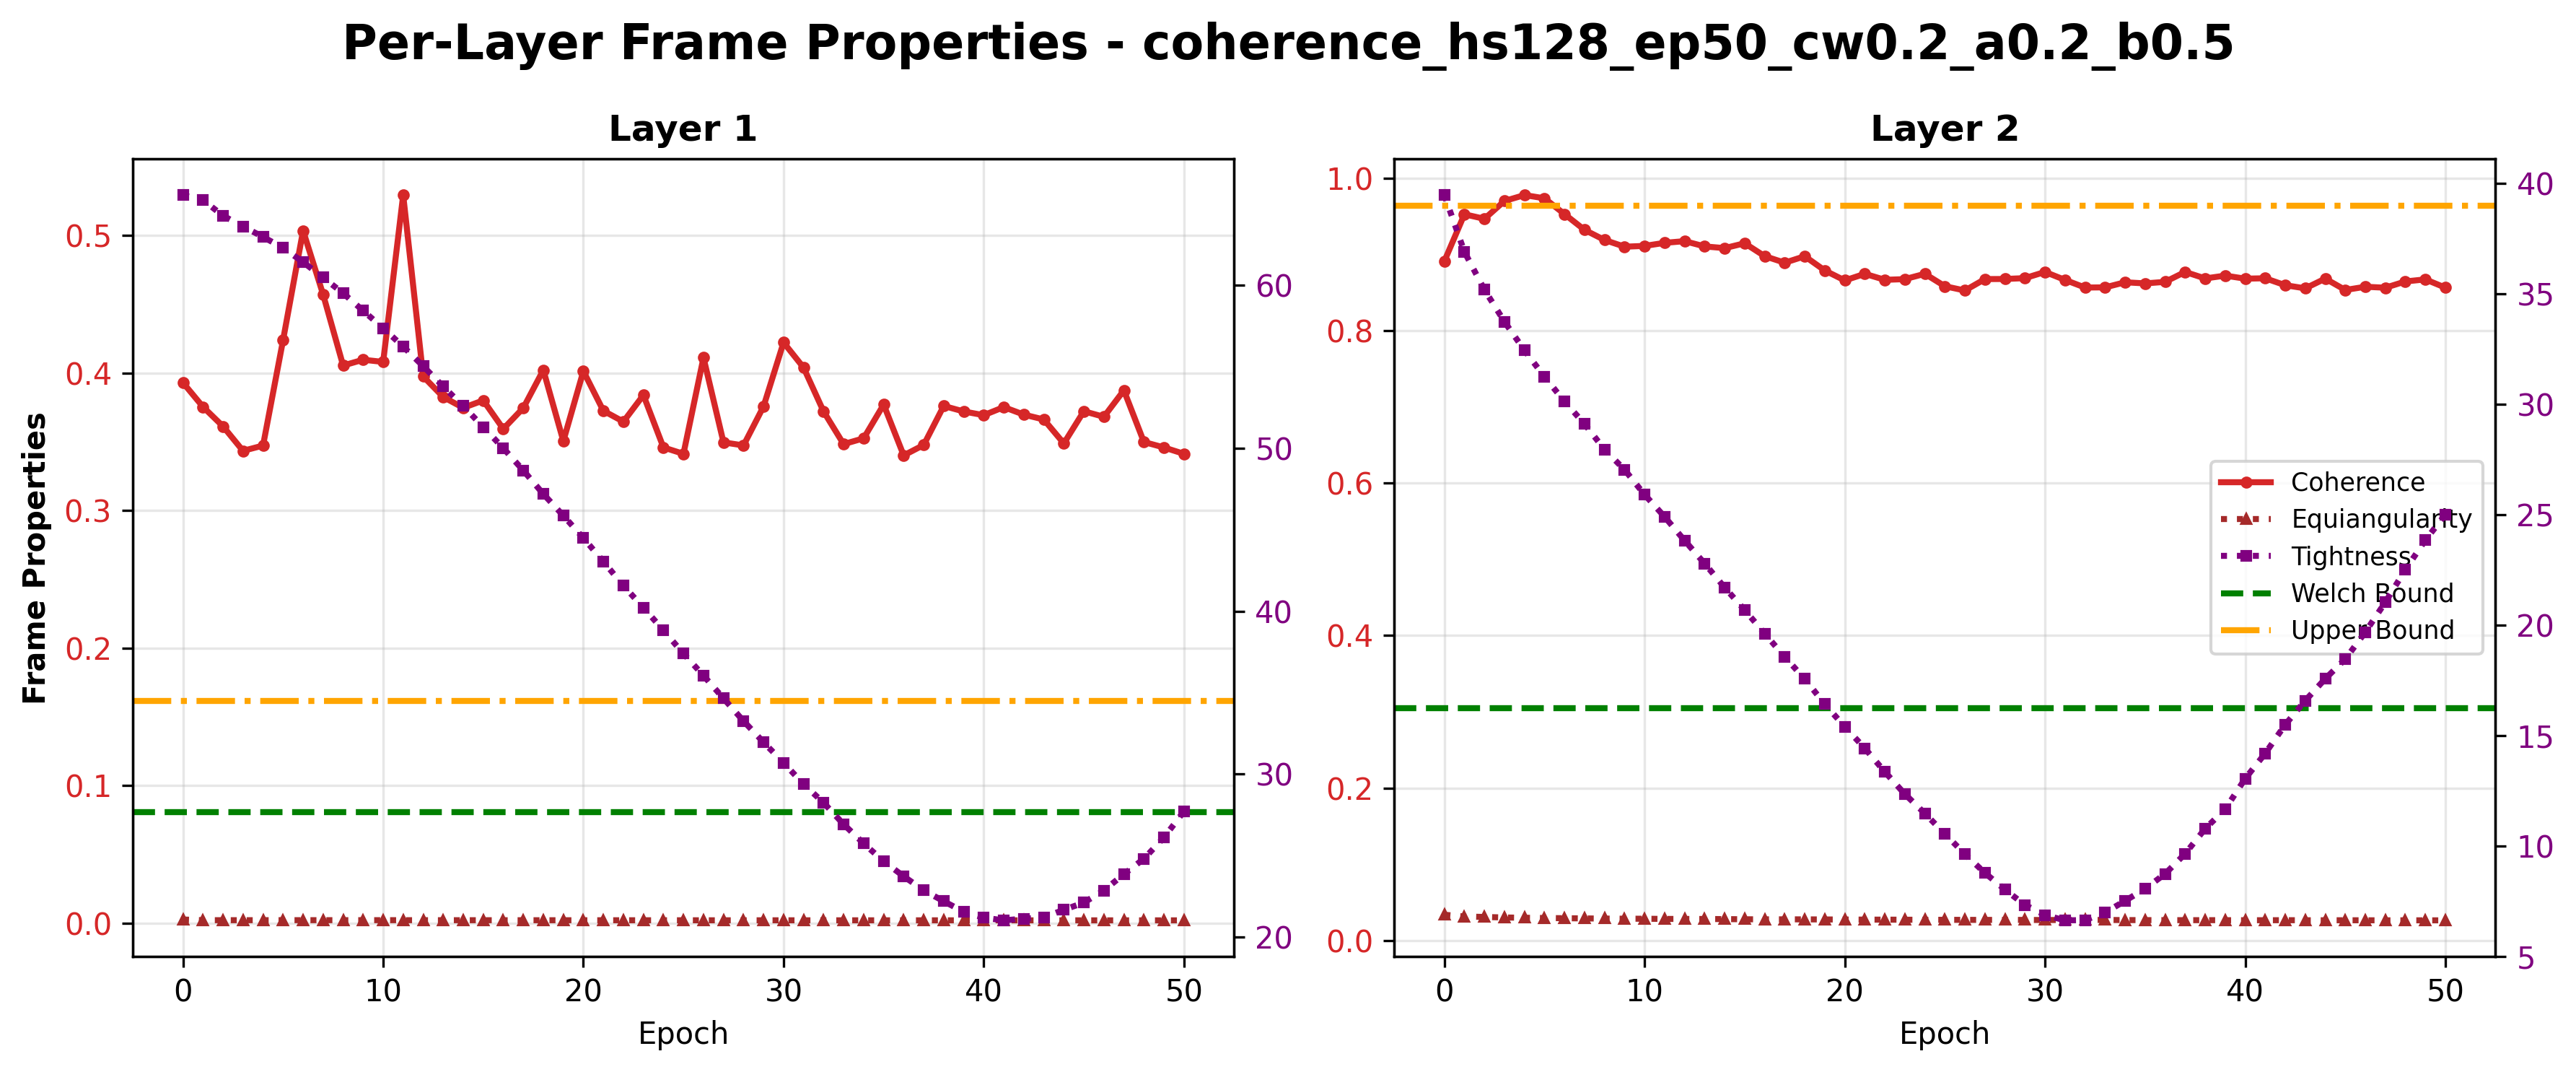
\includegraphics[width=\textwidth,height=0.45\textheight,keepaspectratio]{../plots/mlp/fashion_mnist/hs128_ep50/coherence_hs128_ep50_cw0.2_a0.2_b0.5_coherence_analysis.png}
        \end{minipage}
    \end{figure}
\end{frame}
%--------------------------------------------------------------------------------------
\begin{frame}{Implementation Results: Fashion MNIST}
    \begin{figure}[H]
        \centering
        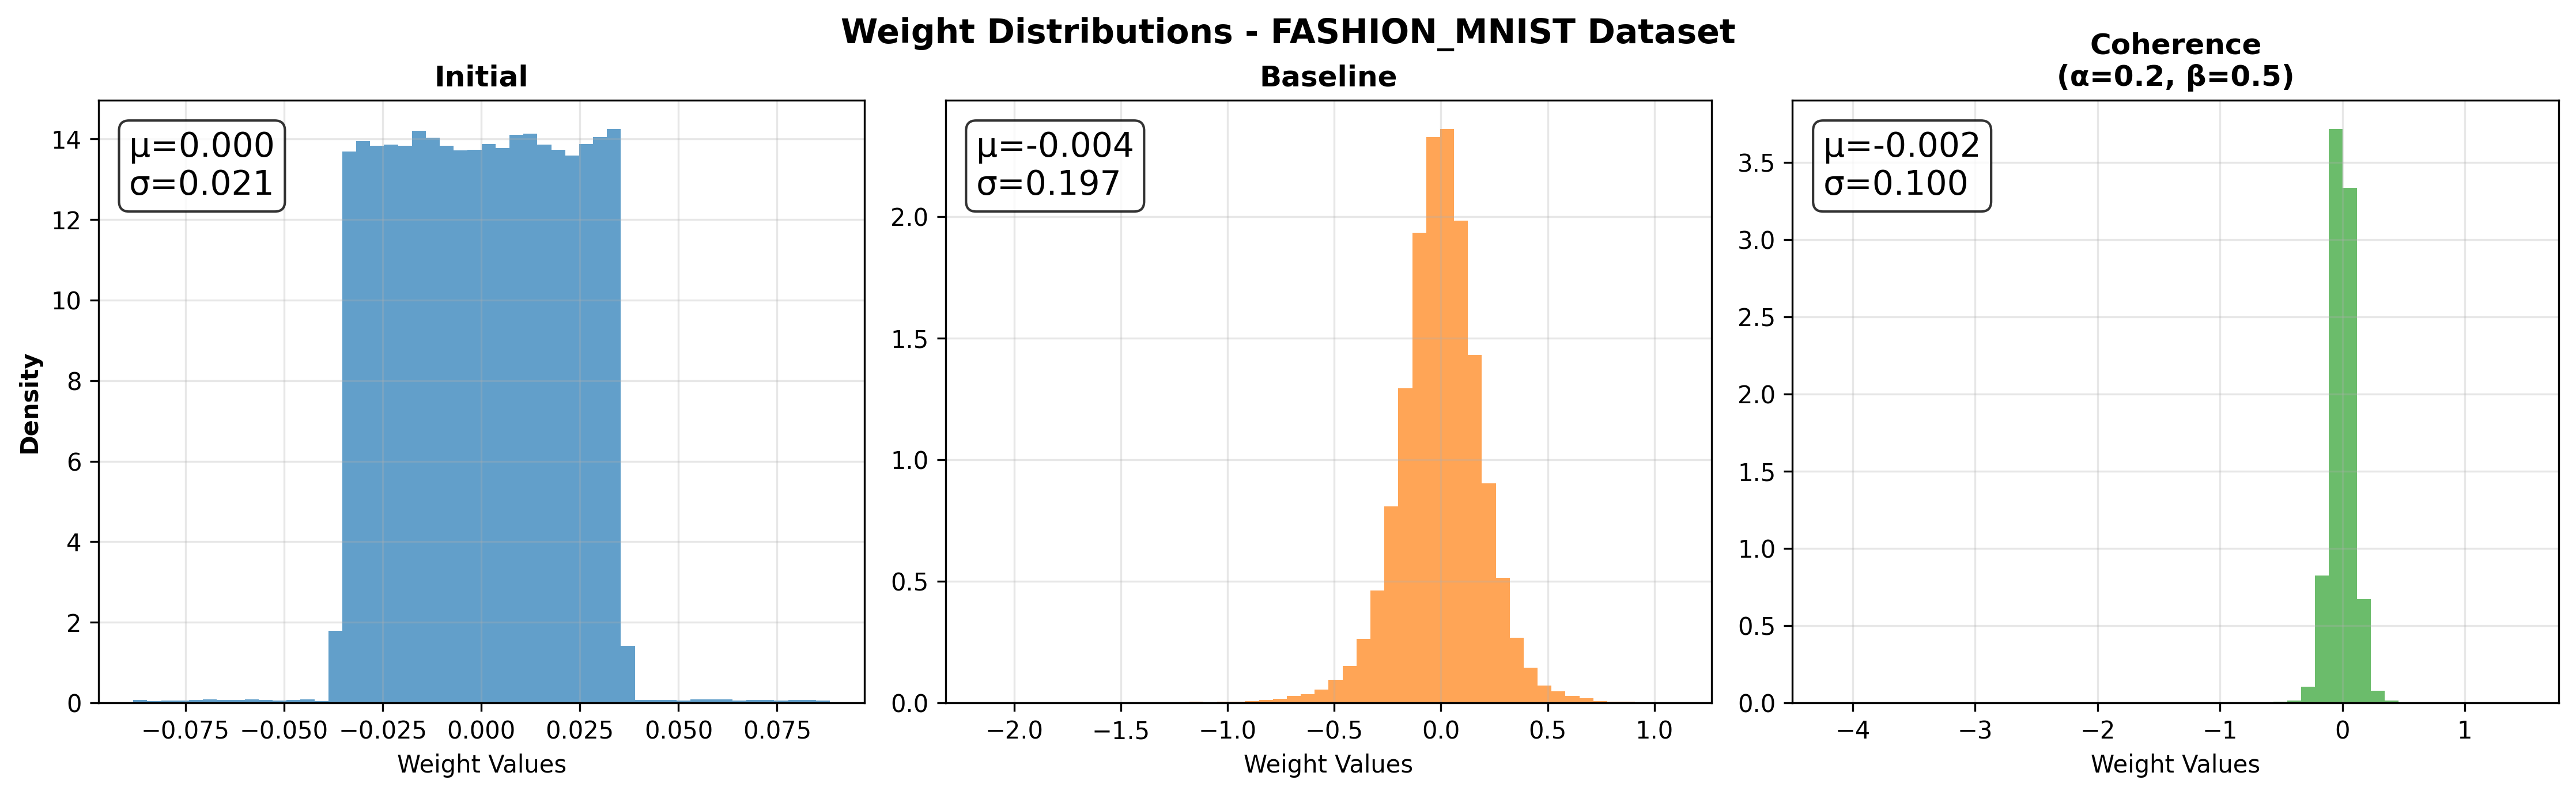
\includegraphics[width=\textwidth]{../plots/mlp/fashion_mnist/hs128_ep50/weights_distribution_baseline.png}
    \end{figure}

	\textbf{Remark:} Regularization = Coherence + Equiangularity + Tightness.
\end{frame}
%--------------------------------------------------------------------------------------
\subsection{Group Theory 101 SpeedRun}
\begin{frame}{Group Theory}

	\begin{block}{\bf Group}
		A group is a {\color{red}\textbf{set}} $G$ with a binary operation $\cdot: G \times G \to G$ that satisfies:
		\begin{itemize}
			\item \textbf{Closure}: $\forall \; g, h \in G$, $g \cdot h \in G$.
			\item \textbf{Associativity}: $\forall \; g, h, \xi \in G$, $(g \cdot h) \cdot\xi = g \cdot (h \cdot \xi)$.
			\item \textbf{Identity Element}: $\exists! \; e \in G$ st. $\forall \; g \in G$, $e \cdot g = g \cdot e = g$.
			\item \textbf{Inverse Element}: $\forall \; g \in G$, $\exists! \; g^{-1} \in G$ st. $g \cdot g^{-1} = g^{-1} \cdot g = e$.
		\end{itemize}
	\end{block}

	\begin{alertblock}{\textbf{(Abbuse of)} Notation}
		\begin{equation*}
			\qquad G = (G, \cdot) \qquad , \qquad hg \equiv h \cdot g, \;\; \forall \; h, g \in G
		\end{equation*}
	\end{alertblock}

	\begin{block}{Group Homomorphism}
		A map $\phi: G \to H$ between groups $G = (G, \cdot)$ and $H = (H, *)$ is a group \textbf{homomorphism} if:
		\begin{equation*}
			\phi(g_1 \cdot g_2) = \phi(g_1) * \phi(g_2) \quad \forall \; g_1, g_2 \in G
		\end{equation*}
	\end{block}

	i.e., the group operation is preserved under the map $\phi$. The ``multiplication'' of elements in $G$ is mapped to the ``composition'' of elements in $H$.

\end{frame}
%--------------------------------------------------------------------------------------
\begin{frame}{Group Theory}

	\begin{block}{Group Action and G-space}
		Given a group $G$, a (left) $G$-space $X$ is a set equipped with a group action $G \times X \to X$, $(g, x) \mapsto g \cdot x$, i.e. a map satisfying the following axioms:
		\begin{itemize}
			\item Identity: $\forall x \in X$: \quad $e \cdot x = x$
			\item Compatibility: $\forall a, b \in G, \forall x \in X$: \quad $a \cdot (b \cdot x) = (a \cdot b) \cdot x$
		\end{itemize}
		If these axioms hold, $G$ acts on the $G$-space $X$.
	\end{block}

	\begin{alertblock}{\textbf{(Abbuse of)} Notation}
		\begin{equation*}
			gx \equiv g \odot x, \;\; \forall \; g \in G, \; \forall \; x \in X
		\end{equation*}
	\end{alertblock}

	\begin{block}{Orbit of a Group}
		Given a group $G$ acting on a set $X$, the \textbf{orbit of an element} $x \in X$ under the group action is the set of all elements that can be reached from $x$ by applying elements of $G$:
		\begin{equation*}
			\mathcal{O}_x = \{g \cdot x : g \in G\} \subseteq X
		\end{equation*}
	\end{block}

	An orbit is then the ``path'' traced by $x$ under the action of $G$.

	Reference: \cite{veefkind_probabilistic_2024}

\end{frame}
%--------------------------------------------------------------------------------------
\begin{frame}{Group Theory}

	\begin{block}{Direct Product Groups}
		Given two groups $(G, \ast)$ and $(H, +)$, the direct product group $(G \times H, \cdot)$ is defined as the Cartesian product $G \times H$ of the two sets, along with the group law:
		\begin{equation*}
			(g_1, h_1) \cdot (g_2, h_2) = (g_1 \ast g_2, h_1 + h_2).
		\end{equation*}

		$K \times H$ is often used as the shorthand notation for the direct product between $H$ and $K$.

	\end{block}

	\begin{block}{Semi-direct Product Groups}
		Considering two groups $(N, *)$ and $(H, +)$ and a group action $\phi : H \times N \to N$ of $H$ on $N$, the semi-direct product group $N \rtimes_\phi H$ is defined as the Cartesian product $N \times H$ with the following binary operation:
		\begin{equation*}
			(n_1, h_1) \cdot (n_2, h_2) = (n_1 * \phi(h_1, n_2), h_1 + h_2)
		\end{equation*}
		and the inverse element:
		\begin{equation*}
			(n, h)^{-1} = (\phi(h^{-1}, n^{-1}), h^{-1})
		\end{equation*}
	\end{block}
\end{frame}
%--------------------------------------------------------------------------------------
\begin{frame}{Group Theory}
	\begin{block}{Homogeneous Space}
		A homogeneous space is a $G$-space with a transitive action on $G$, meaning that for every pair of points $x, y \in X$, there exists an element $g \in G$ such that the action of $g$ on $x$ moves $x$ to $y$. Formally, this is expressed as:
		\begin{equation*}
			\forall x, y \in X, \exists g \in G \text{ s.t. } g \cdot x = y,
		\end{equation*}
	\end{block}

	\textbf{Remark:} All points are connected by a group action, and the whole space is just a single orbit. In other words, the space looks the same from any point.

	\begin{block}{Stabilizer Group}
		Given a group $G$ acting on a set $X$, the \textbf{stabilizer} of an element $x \in X$ under the group action is the set of all group elements that fix $x$:
		\begin{equation*}
			\text{Stab}_G(x) = \{g \in G : g \cdot x = x\}
		\end{equation*}
	\end{block}

	\textbf{Lemma: Let $X$ be a homogeneous space of a group $G$. Then, $X$ can be identified with $G/H$, where $H = \mathrm{Stab}_G(x_0)$ for any $x_0 \in X$.}

\end{frame}
%--------------------------------------------------------------------------------------
\begin{frame}{Group Theory}
	\begin{block}{Linear Group Representation}
		A Linear Group Representation $\rho$ of a group $G$ on a vector space $V$ is a group homomorphism from $G$ to the general linear group $GL(V)$:
		\begin{equation*}
			\rho : G \to GL(V) \quad \text{s.t.} \quad \rho(g_1 \cdot_{G} g_2)v = \rho(g_1) \cdot_{GL(V)}\rho(g_2)v \quad \forall g_1, g_2 \in G, \forall v \in V
		\end{equation*}
		$\rho(g)$ is an invertible linear transformation that preserves the structure of $G$, $V$.
	\end{block}

	\begin{block}{Matrix Representation}
		A matrix representation is a linear group representation, with a choice of basis, that acts on a finite dimensional vector space $\mathbb{R}^d$ such that all group elements are represented as concrete matrices $\mathbf{D}(g) \in GL(\mathbb{R}^d)$. {\color{red} \textbf{Used in practice.}}
	\end{block}

	\begin{block}{Left Regular Representation}
		For a group $G$ and function $f : G \to Y$, with $Y$ a field, the left-regular representation $\mathscr{L}_g$ \textbf{acts} on $f$ by ``shifting'' its domain. For a group element $g \in G$, the action $\mathscr{L}_g$ on $f$ results in a new function $\mathscr{L}_g f : G \to Y$, $\mathscr{L}_g f \in L^2(G)$, defined by:
		\begin{equation*}
			(\mathscr{L}_g f)(h) = f(g^{-1}h) \quad \forall \; h, g \in G
		\end{equation*}
	\end{block}

\end{frame}
%--------------------------------------------------------------------------------------
\begin{frame}{Group Theory}

	\begin{block}{Affine Groups}
		Affine groups $G = \mathbb{R}^d \rtimes H$ are a class of groups that are the semidirect product of a group $H \subseteq GL(\mathbb{R}^d)$ acting on $\mathbb{R}^d$, with $GL(\mathbb{R}^d)$ the group of general linear transformations acting on $\mathbb{R}^d$.
	\end{block}

	\begin{block}{Example: Roto-translation Group}
		The \textbf{roto-translation group} $SE(2)$ is the Special Euclidean Group in 2D, consisting of all combinations of translations and rotations in the plane. It can be defined as:
		\begin{equation*}
			SE(2) = \mathbb{R}^2 \rtimes SO(2)
		\end{equation*}

		Each element is represented as $(x, \theta)$ where $x \in \mathbb{R}^2$ is a translation vector and $\theta \in SO(2)$ is a rotation angle. The group operation is:
		\begin{equation*}
			(x_1, \theta_1) \cdot (x_2, \theta_2) = (\mathbf{R}_{\theta_1} x_2 + x_1, \theta_1 + \theta_2)
		\end{equation*}

		where $\mathbf{R}_{\theta}$ is the 2D rotation matrix for angle $\theta$.
	\end{block}

\end{frame}
%--------------------------------------------------------------------------------------
\begin{frame}{Group Theory}

	\begin{block}{Equivariance}
		Given a group $G$ and two sets $X$ and $Y$ that are acted on by $G$, a map (e.g., a layer in a neural network) $f : X \to Y$ is equivariant iff
		\begin{equation*}
			\forall x \in X, \forall g \in G: \quad f(g \cdot x) = g \cdot f(x)
		\end{equation*}
	\end{block}

	\begin{itemize}
		\item Equivariance guarantees that input transformations result in predictable output transformations.
		\item Input transformations shift information rather than losing it, so no information is lost.
		\item Enables weight sharing across group transformations - features detected at one location/pose are equally detected at others.
	\end{itemize}

	\begin{block}{Invariance}
		Given a group $G$ and two sets $X$ and $Y$ that are acted on by $G$, a map $f : X \to Y$ is invariant iff
		\begin{equation*}
			\forall x \in X, \forall g \in G: \quad f(g \cdot x) = f(x)
		\end{equation*}
	\end{block}

	\begin{itemize}
		\item Output remains constant for all inputs related by group actions.
	\end{itemize}
\end{frame}
%--------------------------------------------------------------------------------------
\subsection{Group Equivariant Neural Networks}
\begin{frame}{Equivariant Neural Networks}

	In the basic case, a neural network is a function that maps an input \( f \) to an output function \( g \) via a series of linear maps \( \mathcal{N}_i \) followed by non-linear activation functions, which can be expressed as:

	\begin{equation}
		g = \mathcal{N}(f) = \mathcal{N}_L \circ \mathcal{N}_{L-1} \circ \ldots \circ \mathcal{N}_1(f)
	\end{equation}

	\begin{block}{Theorem: Dunford-Pettis: Linear bounded maps are integral transforms}
		Let \( K : L^2(X) \rightarrow L^2(Y) \) be a linear and bounded operator that maps between spaces of feature maps \( L^2(X) \) and \( L^2(Y) \). Then there exists a kernel \( k \in L^1(Y \times X) \) such that \( K \) is an integral transform via:
		\begin{equation*}
			(Kf)(y) = \int_X k(y, x) f(x) \, d\mu_X(x)
		\end{equation*}
		with \( f \in L^2(X) \), and \( d\mu_X \) a ``Radon measure'' on \( X \).
	\end{block}

	\textbf{Vectors:}
	\begin{equation}
		f^{l+1} = Wx \quad \leftrightarrow \quad f^{l+1}_j = \sum_{i=1}^{N_l} w_{ji} x^l_i
	\end{equation}

	\textbf{Signals:}
	\begin{equation}
		f^{l+1} = K f^l \quad \leftrightarrow \quad f^l(y) = \int_X k(y, x) f^l(x) d\mu_X(x)
	\end{equation}

\end{frame}
%--------------------------------------------------------------------------------------
\begin{frame}{Types of Equivariant Neural Networks}

	\begin{block}{Theorem: Equivariant linear layers on homogeneous spaces}

		Let $\mathcal{K} : L^2(X) \rightarrow L^2(Y)$ be a linear and bounded operator. Let $X, Y$ be homogeneous spaces on which a (Lie) group $G$ acts transitively, and let $d\mu_X$ be a ``Radon measure'' on $X$. Suppose $\mathcal{K}$ is equivariant to the group $G$ via $L^Y_g \circ \mathcal{K} = \mathcal{K} \circ L^X_g$, with $L^X_g$ and $L^Y_g$ are the left-regular representations of $G$ on $L^2(X)$ and $L^2(Y)$, respectively. \textbf{Then:}

		\begin{enumerate}
			\item $\mathcal{K}$ is a group convolution given by:
			      \begin{equation*}
				      (\mathcal{K}f)(y) = \int_X \dd\mu_X(x) \dv{\mu_X(g_y^{-1} x)}{\mu_X(x)} k(g_y^{-1} x) f(x)
			      \end{equation*}
			      for any $g_y \in G$ such that $y = g_y y_0$ for some fixed origin $y_0 \in Y$.

			\item The kernel must satisfy the symmetry constraint:
			      \begin{equation*}
				      k(x) = \dv{\mu_X(g_y^{-1} x)}{\mu_X(x)} k(h^{-1} x)
			      \end{equation*}
			      for any $h \in H = \mathrm{Stab}_G(y_0)$, and any $x \in X$.
		\end{enumerate}
	\end{block}

	Reference: \cite{bekkers_introduction_2021}

\end{frame}
%--------------------------------------------------------------------------------------
\begin{frame}{Types of Equivariant Neural Networks}

	\textbf{Isotropic $\mathbb{R}^d$ Convolutions ($X = Y = \mathbb{R}^d$)}

	An isotropic $\mathbb{R}^d$ convolution layer maps between planar signals $L_2(\mathbb{R}^d)$ with $\mathcal{K}$ a planar correlation given by
	\begin{equation}
		(\mathcal{K}f)(y) = \int_{\mathbb{R}^d} \frac{1}{|\det h|} k(\mathbf{x} - \mathbf{y}) f(\mathbf{x}) \dd\mathbf{x}
	\end{equation}
	and in which $k$ satisfies
	\begin{equation*}
		\forall h \in H : \quad k(\mathbf{x}) = \frac{1}{|\det h|} k(h^{-1} \mathbf{x})
	\end{equation*}

	\textbf{Lifting Layer ($X = \mathbb{R}^d$, $Y = G$)}

	A lifting layer maps from planar signals $L_2(\mathbb{R}^d)$ to signals $L_2(G)$ on the group $G$, with $\mathcal{K}$ a lifting correlation given by
	\begin{equation}
		(\mathcal{K}f)(g) = \int_{\mathbb{R}^d} \frac{1}{|\det h|} k(g^{-1}\tilde{\mathbf{x}}) f(\tilde{\mathbf{x}}) \dd\tilde{\mathbf{x}}
	\end{equation}

	\textbf{Group Convolution Layer ($X = Y = G$)}

	A group convolution layer maps between $G$-feature maps in $L_2(G)$, with $\mathcal{K}$ a group correlation given by
	\begin{equation}
		(\mathcal{K}f)(g) = \int_G k(g^{-1}\tilde{g}) f(\tilde{g}) \dd\tilde{g}
	\end{equation}
	with $\dd\tilde{g}$ the left ``Haar'' measure on $G$.

\end{frame}
%--------------------------------------------------------------------------------------
\begin{frame}{Example: Roto-translation lifting convolutional layer}

	Let $G = SE(2) = \mathbb{R}^2 \rtimes SO(2)$ be the roto-translation group in 2D. The lifting correlation of a convolutional layer represented by the linear operator $\mathcal{K}^{l}: \mathbb{R}^2 \to SE(2)$ on a function $f \in L^2(\mathbb{R}^2)$ is:

	\begin{equation*}
		\begin{split}
			f^{l+1} (g) & = (\mathcal{K}^{l} f)(g)                                                   \\
			            & = (k *_{SE(2)} f)(g)                                                       \\
			            & = \braket{\mathscr{L}_x \mathscr{L}_{\theta} k}{f^{l}}_{L^2(\mathbb{R}^2)} \\
			            & = \braket{\mathscr{L}_x k_{\theta}}{f^{l}}_{L^2(\mathbb{R}^2)}             \\
			            & = (k_{\theta} *_{\mathbb{R}^2} f)(x)
		\end{split}
	\end{equation*}

	where $f^{l+1} \in L^2(SE(2))$, $g = (x, \theta)$, $x \in \mathbb{R}^2$ and $\theta \in SO(2)$.

	\sectionvspace

	\textbf{Note:} the lifting convolution and G-convolutions can be obtained by first precomputing a filter bank of transformed kernels and then apply them to the input signal via the usual planar correlation (GPU optimized) on $\mathbb{R}^2$, {\bf or $\mathbb{Z}^2$ to be precise in the discrete practical case.} Here, the transformed kernel is obtained via $k_\theta(x) = k(\mathbf{R}_{\theta}^{-1} x)$. Computationally, this says that to get the transformed kernel at the point $x$, we need to do a lookup in the original kernel $k$ at the point $\mathbf{R}_{\theta}^{-1} x$, which is the unique point that gets mapped to $x$ by $\theta$.

\end{frame}
%--------------------------------------------------------------------------------------
\subsection{Frame Theory Primer}
\begin{frame}{Frame Theory}

	\begin{block}{Matrix Definition of a Frame}
		The frame condition can be written as:
		\begin{equation*}
			A \|x\|^2 \leq x^T X X^T x  = \|X^T x\|^2 \leq B \|x\|^2.
		\end{equation*}
		This follows because:
		\begin{equation*}
			\sum_{i=1}^n |\langle x, f_i \rangle|^2 = \sum_{i=1}^n (x^T f_i)^2 = x^T \left(\sum_{i=1}^n f_i f_i^T\right) x  =x^T X X^T x = \|X^T x\|^2.
		\end{equation*}
	\end{block}

	\begin{block}{Frame Operator}
		Given a frame $\{f_i\}_{i=1}^n$, the \textbf{frame operator} $S: H \to H$ is defined by
		\begin{equation*}
			Sx = \sum_{i=1}^n \langle x, f_i \rangle f_i.
		\end{equation*}

	\end{block}

	Using Dirac notation, we can write:
	\begin{equation*}
		S = \sum_{i=1}^n \ket{f_i} \bra{f_i} \implies S \ket{x} = \sum_{i=1}^n \braket{x}{f_i} \ket{f_i}
	\end{equation*}

\end{frame}
%--------------------------------------------------------------------------------------
\begin{frame}{Frame Theory}

	\begin{block}{Outer Product Decomposition of the Frame Operator}
		The frame operator can be written as
		\begin{equation*}
			S = XX^T = \sum_{i=1}^n f_i f_i^T
		\end{equation*}

		\textbf{Proof:}
		Recall that the standard basis vector $e_i \in \mathbb{R}^n$ satisfies $(e_i)_j = \delta_{ij}$ such that $X = \sum_{i=1}^n f_i e_i^T$, because $f_i e_i^T$ produces a matrix with $f_i$ in the $i$-th column and zeros elsewhere.

		Now compute the frame operator:

		\begin{align*}
			XX^T & = \left( \sum_{i=1}^n f_i e_i^T \right) \left( \sum_{j=1}^n e_j f_j^T \right)^T          \\
			     & = \left( \sum_{i=1}^n f_i e_i^T \right) \left( \sum_{j=1}^n e_j f_j^T \right)            \\
			     & = \sum_{i=1}^n \sum_{j=1}^n f_i (e_i^T e_j) f_j^T = \sum_{i=1}^n f_i f_i^T \quad \square
		\end{align*}
	\end{block}
\end{frame}
%--------------------------------------------------------------------------------------
\begin{frame}{Frame Theory}

	\begin{block}{Tight Frame}
		A frame $\{f_i\}_{i=1}^n$ is called a \textbf{tight frame} if the frame bounds satisfy $A = B$. In this case, the frame inequality becomes:
		\begin{equation*}
			\sum_{i=1}^n |\langle x, f_i \rangle|^2 = A \|x\|^2 \quad \forall x \in \mathcal{H}
		\end{equation*}
	\end{block}

	\begin{block}{Key Properties of Tight Frames}
		\begin{itemize}
			\item \textbf{Optimal reconstruction}: Equal frame bounds provide stability
			\item \textbf{Energy preservation}: Perfect energy balance across all directions
			\item \textbf{Simplified analysis}: Frame operator becomes a scalar multiple of identity
			\item \textbf{Connection to equiangular frames}: Combined with equiangularity, achieves Welch bound
		\end{itemize}
	\end{block}

\end{frame}
%--------------------------------------------------------------------------------------
\begin{frame}{Frame Theory}

	\begin{block}{Frame Operator of Tight Frames}
		Let $\{f_i\}_{i=1}^n$ be a tight frame in $\mathbb{R}^m$, and let $X \in \mathbb{R}^{m \times n}$ be the matrix of frame vectors. Then:
		\begin{equation*}
			XX^T = A I_m
		\end{equation*}
	\end{block}

	\begin{block}{Proof}
		Let $S = XX^T$ be the frame operator. Since the frame is tight with bound $A$:
		\begin{align*}
			\langle Sx, x \rangle &= \sum_{i=1}^n |\langle x, f_i \rangle|^2 = A \|x\|^2 = \langle A x, x \rangle
		\end{align*}
		Thus, for all $x \in \mathbb{R}^m$: $\langle (S - A I)x, x \rangle = 0$.
		
		This implies $S = A I_m$ by the polarization identity and positive-definiteness of $S$. \qed
	\end{block}

\end{frame}
%--------------------------------------------------------------------------------------
\begin{frame}{Frame Theory}

	\begin{block}{Tight Frame Bound for Unit Vectors}
		If the frame vectors are unit norm and the frame is tight, then:
		\begin{equation*}
			A = \frac{n}{m}
		\end{equation*}
	\end{block}

	\begin{block}{Proof}
		Taking the trace of both sides of $XX^T = A I_m$:
		\begin{align*}
			\text{Tr}(XX^T) &= \sum_{i=1}^n \text{Tr}(f_i f_i^T) = \sum_{i=1}^n \|f_i\|^2 = n \\
			\text{Tr}(A I_m) &= A \cdot m
		\end{align*}
		Equating: $A m = n \Rightarrow A = \frac{n}{m}$. \qed
	\end{block}

	\begin{block}{Geometric Interpretation}
		For unit-norm tight frames, each coordinate direction receives exactly $\frac{n}{m}$ units of total energy from all frame vectors, providing perfect energy balance.
	\end{block}

\end{frame}
%--------------------------------------------------------------------------------------
\end{document}